%\documentclass[a4paper,12pt,twoside]{book}
\documentclass[12pt,times]{report}
\usepackage{mathptmx}%This package supersedes times and mathptm
\usepackage[a4paper,right=2.54cm,left=2.54cm,top=2.54cm,bottom=2.54cm]{geometry}

% Nuevos paquetes
\usepackage[utf8]{inputenc}
\usepackage{amsmath}
\usepackage{multicol} 
\usepackage{float}
\usepackage{titlesec}
\usepackage[utf8]{inputenc}
\usepackage{geometry}
\usepackage{array}
\usepackage[table]{xcolor}
\geometry{margin=1in}
\newcolumntype{L}[1]{>{\raggedright\arraybackslash}p{#1}}
\newcolumntype{R}[1]{>{\raggedleft\arraybackslash}p{#1}}

% \titlespacing*{\chapter}{0pt}{-25pt}{10pt}


%%%%paquete para usar citas de diferentes formatos
%%%%%%%%%%%%%%%%%%%%%%%%%%%%%%%%%
%%add al indice
%\usepackage[nottoc,numbib]{tocbibind}
%\usepackage[authoryear,round]{natbib}

%%%%%%%%%%%%%%%%%%%%%%%%%%%%%5
%%%%Paquete para alinear texto
\usepackage{longtable}
\usepackage{array, multirow, multicol}
\usepackage{ragged2e}
\usepackage{multirow}
\usepackage{makecell}
\usepackage{rotating}
\usepackage{siunitx} % To align the numbers later on
\usepackage[table,xcdraw]{xcolor}
\usepackage{colortbl, color}
\usepackage{tabularx}
\definecolor{Gray}{gray}{0.9}
\definecolor{orange}{rgb}{1,0.647,0}
\definecolor{turq3}{rgb}{0.54, 0.81, 0.94}
\definecolor{turq}{rgb}{0.63, 0.79, 0.95}
\definecolor{bluejean}{rgb}{0.03, 0.27, 0.49}

\usepackage[utf8]{inputenc}
\usepackage{csquotes}
\usepackage[spanish]{babel}

\usepackage[style=apa,
%hyperref=auto,
%citestyle=authoryear,
natbib=true,
backend=biber]{biblatex}
%backend=biber

%\addbibresource{biblio/references.bib}

\addbibresource{tesisblx.bib} % Ajusta esto a tu archivo BibTeX
\nocite{*}

%\usepackage{biblatex}
%paquete para hiperlinks entre citas e imagenes
%%%%%%%%%%%%%%%%%%%%%%%%%%%%%%%%%
\usepackage[colorlinks=true,
citecolor=black, %cambiar el color de las citas citecolor=blue
urlcolor=cyan,
bookmarks=true,
linkcolor=blue]{hyperref}
%pdftitle={Tesis-nombre-alumno},
%pdfauthor={autor nombres}]{hyperref}

\usepackage{url}
\usepackage{amssymb}
\usepackage{graphicx} % for improved inclusion of graphics
%\usepackage{wrapfig} % to include figure with text wrapping around it
\usepackage[margin=10pt,font=small,labelfont=bf]{caption} % for improved layout of figure captions with extra margin, smaller font than text
\usepackage{eucal}
%\usepackage[usenames, dvipsnames]{color}
\usepackage[perpage]{footmisc}
%\usepackage[round, sort]{natbib}
\usepackage{ifthen}
\usepackage{multicol} % for pages with multiple text columns, e.g. References
\setlength{\columnsep}{20pt} % space between columns; default 10pt quite narrow
\usepackage[nottoc]{tocbibind} % correct page numbers for bib in TOC, nottoc suppresses an entry for TOC itself
\usepackage{appendix}



\usepackage{float}



%%%----Modificar encabezado y pie de pagina
%%%%%%%%%%%%%%%%%%%%%%%%%%%%%%%%%%%%%%%%%%%%%%%%%%%%%%%%%%%%%%%%%%%%%
\usepackage{fancyhdr} % for better header layout
\newcommand{\changefont}{%
	\fontsize{9pt}{1.5pt}\selectfont
}
\pagestyle{fancy}
\fancyhf{} %% delete default configuration of page
%%\setlength\headheight{15pt}
\fancyhead[L]{\changefont Tesis II}
\fancyhead[R]{\changefont \leftmark}
%%\fancyfoot[L]{\leftmark}
\fancyfoot[R]{\thepage}

%%%%%%%%%%%%%%%%%%%%%%%%%%%%%5
%%%% Configuracion de los parrafos
%\usepackage{setspace}
%\onehalfspacing
%\linespread{1.25} 
\setlength{\parindent}{0.5in} %%sangria
\setlength{\parskip}{3mm}  %%espacio entre parrafos
\linespread{1.3} %This equals 1.5 linespacing in Word
%%%% nuevo parrafo
%%%%%%%%%%%%%%%%%%%%%%%%%%%%%5
%%%% Centrar valores de una tabla
\usepackage{array}
%%CENTRADO HORIZONTAL
\newcolumntype{P}[1]{>{\centering\arraybackslash}p{#1}}
%%CENTRADO VERTICAL
\newcolumntype{M}[1]{>{\centering\arraybackslash}m{#1}}
%%TABLAS LONGTABLE
\newcolumntype{L}[1]{>{\raggedright\let\newline\\\arraybackslash\hspace{0pt}}m{#1}}
\newcolumntype{C}[1]{>{\centering\let\newline\\\arraybackslash\hspace{0pt}}m{#1}}
\newcolumntype{R}[1]{>{\raggedleft\let\newline\\\arraybackslash\hspace{0pt}}m{#1}}


%%%%%%%%%%%%%%%%%%%%%%%%%
\usepackage{xparse}
\usepackage{expl3}
%%%%funcion de reemplazar regex
\ExplSyntaxOn
\NewDocumentCommand{\replace}{mmm}
{
	\marian_replace:nnn {#1} {#2} {#3}
}

\tl_new:N \l_marian_input_text_tl
\tl_new:N \l_marian_search_tl
\tl_new:N \l_marian_replace_tl

\cs_new_protected:Npn \marian_replace:nnn #1 #2 #3
{
	\tl_set:Nn \l_marian_input_text_tl { #1 }
	\tl_set:Nn \l_marian_search_tl { #2 }
	\tl_set:Nn \l_marian_replace_tl { #3 }
	\regex_replace_all:nnN { \b\u{l_marian_search_tl}\b } { \u{l_marian_replace_tl} } \l_marian_input_text_tl
	\tl_use:N \l_marian_input_text_tl
}
\ExplSyntaxOff

%%%%%%%%%%%%%%%%%%%%%%%%%%%%%%%%%%%%%%
\usepackage{amsmath}
\numberwithin{equation}{chapter} %%enumerar ecuaciones
\renewcommand{\theequation}{Ecuación \thechapter.\arabic{equation}}   
\usepackage{mathtools, nccmath, cool}
%%%Configuraciones de biblatex

%\include{biblio/config}
\makeatletter
\let\abx@macro@citeOrig\abx@macro@cite
\renewbibmacro{cite}{%
	\bibhyperref{%
		\let\bibhyperref\relax\relax%
		\abx@macro@citeOrig%
	}%
}
\let\abx@macro@textciteOrig\abx@macro@textcite
\renewbibmacro{textcite}{%
	\bibhyperref{%
		\let\bibhyperref\relax\relax%
		\abx@macro@textciteOrig%
	}%
}%

\makeatother

%%%%%%%%%%%%%%%%%%%%%%%%%%%%%%%%%%%%%%%%%%%
\begin{document}
	\begin{titlepage}
		\begin{center}
		%%%cargar imagen
			
\includegraphics[width=0.45\textwidth]{images_repo/esanlogomin}
			\vspace*{2cm} \\
			UNIVERSIDAD ESAN \vspace*{1ex} \\
			FACULTAD DE INGENIERÍA \vspace*{1ex} \\
			INGENIERÍA DE TECNOLOGÍAS DE INFORMACIÓN Y SISTEMAS\vspace*{8ex} \\
			\textbf{Predicción de Demanda mediante Modelos de Series Temporales y Machine Learning para la Optimización del Reabastecimiento en una Empresa Retail}
			\vspace*{8ex}\\	
			Trabajo de suficiencia profesional presentado en satisfacción parcial de los requerimientos para obtener el título profesional de ingeniero de tecnologías de información y sistemas
			\vspace*{8ex} \\	
			Zacarías Kevin Paucar Tello \\
			Jerson Walter Toledo Flores \\
			Jean Pierre Castro Acuña \\
			Asesor: Marks Calderón		
			\vfill
			
			Lima, \today 
			
		\end{center}
	\end{titlepage}
	%%cambiar nombres de objetos para el indice y otros
		\renewcommand{\listfigurename}{Índice de Figuras}
		\renewcommand{\tablename}{Tabla}
		\renewcommand{\listtablename}{Índice de Tablas}
	
	
		\thispagestyle{plain}
\begin{center}
	\vspace*{1.5cm}
	{\Large \bfseries  Resumen}
\end{center}
\vspace{0.5cm}
Para optimizar la toma de decisiones en la compra de productos de la empresa, es fundamental desarrollar un modelo predictivo de demanda que integre datos históricos de ventas con información relevante, como precios, cantidades, días festivos, número de transacciones y otros factores. Este proceso comienza con una recopilación exhaustiva de datos, seguida de un análisis exploratorio para identificar patrones y tendencias significativas.  

La selección de características permite determinar las variables que tienen mayor impacto en la demanda. Posteriormente, se emplean técnicas de modelado predictivo, como regresión lineal, redes neuronales, máquinas de soporte regresion (SVR), Random Forest, ARIMA, Prophet, entre otros modelos de forecasting y aprendizaje automático, para predecir el volumen futuro de ventas. Una vez entrenado, el modelo se valida rigurosamente para garantizar su precisión.  
Tras su implementación, es crucial realizar un seguimiento continuo del modelo para ajustarlo y optimizar las predicciones frente a cambios en el mercado y otros factores relevantes. Esto permite mejorar la gestión de decisiones estratégicas y diseñar políticas de precios más efectivas.  
La investigación se centra en el uso de modelos de series de tiempo para identificar las áreas con mayor volumen de ventas, maximizando así los ingresos potenciales. Los modelos de series temporales son herramientas analíticas que permiten analizar y predecir patrones en datos secuenciales a lo largo del tiempo.  

Para llevar a cabo este enfoque, es esencial recopilar datos detallados de ventas por familia de productos, incluyendo información como volúmenes de ventas diarios, semanales o mensuales, ingresos generados y factores externos, como promociones, eventos especiales, fines de semana o días festivos. Mediante el análisis de estos datos, es posible identificar patrones y tendencias que faciliten pronósticos precisos para la empresa Donna S.A.C.  

El análisis de series de tiempo implica estudiar la estructura temporal de los datos, considerando factores como tendencia, estacionalidad y variaciones aleatorias. Con esta comprensión, se aplican modelos estadísticos y técnicas de pronóstico para estimar el comportamiento futuro de las ventas. Utilizando este enfoque, la empresa puede obtener estimaciones confiables y precisas que impulsen una mejor toma de decisiones estratégicas y operativas.\\

\textbf{Palabras claves: } Predicción, Ventas, Machine Learning, Regresión
		\thispagestyle{plain}
\begin{center}
	\vspace*{1.5cm}
	{\Large \bfseries  Abstract}
\end{center}
\vspace{0.5cm}
This research aimed to implement time series and Machine Learning models to improve decision-making in the supplier replenishment process of Donna S.A.C. The problem addressed is related to the difficulty of adequately estimating product demand, especially in contexts where sales variability, seasonality, and the short shelf life of certain products may lead to overstock, stockouts, economic losses, and purchasing decisions based mainly on the administrator's experience.

The research was developed under an applied and quantitative approach, using the company's historical sales data as the main source of information. The methodological process included data acquisition and understanding, information preprocessing, selection of relevant variables, construction of temporal features, training of predictive models, comparative evaluation, and deployment of the solution. During preprocessing, activities such as data cleaning, outlier treatment, sales aggregation by date, selection of relevant columns, and generation of variables such as day of the week, month, sales lags, and moving averages were carried out.

To evaluate model performance, metrics such as MAE, MSE, RMSE, MAPE, and the coefficient of determination $R^2$ were used, with the purpose of comparing the generated predictions against the actual values. The results obtained made it possible to identify the models that presented the best overall performance for each category, as they recorded lower error levels and a better fit compared to the other evaluated models. Likewise, a support solution was developed through a system that allows users to visualize predictions, compare actual and forecasted sales, and facilitate replenishment planning.

Finally, it is concluded that the implementation of predictive models contributes to transforming historical sales data into useful information for operational decision-making. The proposed solution helps reduce uncertainty in product purchasing, optimize the supply budget, and reduce risks associated with excess or insufficient inventory, thereby strengthening the efficiency of the supplier ordering process at Donna S.A.C.


\textbf{Keywords: } Forecasting, Sales, Machine Learning, Regression
		\thispagestyle{plain}
\begin{center}
	\vspace*{1.5cm}
	{\Large Para mi familia y amigos}
\end{center}


		\include{0/agradecimientos}
	
	% outline
		\tableofcontents            % print the table of contents
	
	%: ----------------------- contents ------------------------
	
		\setcounter{secnumdepth}{3} % organisational level that receives a numbers
		\setcounter{tocdepth}{3}    % print table of contents for level 3
	
	% levels are: 0 - chapter, 1 - section, 2 - subsection, 3 - subsection
	
	
	%: ----------------------- list of figures/tables ------------------------
	
		\listoffigures	% print list of figures
	
		\listoftables  % print list of tables
	
	
	
\chapter{PLANTEAMIENTO DEL PROBLEMA}
\section{Descripción de la Realidad Problemática}

A nivel mundial, la predicción de la demanda de productos perecibles enfrenta desafíos significativos debido a la complejidad de los factores externos, la disponibilidad limitada de datos completos y precisos, la variabilidad en la vida útil de los productos, la naturaleza estática de muchos modelos predictivos, los desafíos logísticos y de distribución, así como los costos asociados con errores en las predicciones. Mejorar la rentabilidad en este contexto requiere el desarrollo de modelos más sofisticados que consideren estos desafíos y una gestión efectiva de la cadena de suministro para minimizar los riesgos financieros asociados con la incertidumbre en la demanda. Por ejemplo, un estudio realizado en China examinó la importancia de la precisión en las predicciones para evitar pérdidas en la industria de alimentos perecibles en el contexto de la rentabilidad empresarial (\cite{foodbank}). Además, en un trabajo llevado a cabo en Estados Unidos, se destacó la influencia de factores externos como las condiciones climáticas y los cambios en los hábitos de consumo en la demanda de productos perecibles, lo cual impacta directamente en la rentabilidad de las empresas. Estas investigaciones reflejan la preocupación global por mejorar la capacidad predictiva en el ámbito de los productos perecibles para optimizar la rentabilidad en un contexto empresarial cada vez más competitivo.

En este contexto, la aplicación de minería de datos y modelos de pronóstico se presenta como una solución estratégica. ``Bajo esta premisa, la utilización de pronósticos en estos productos ayudará a planificar de mejor forma el proceso de abastecimiento, a través de métodos cuantitativos. Para llevar a cabo este estudio se aplica un análisis de autocorrelación a todas las series de tiempo, con el fin de verificar la estacionalidad o aleatoriedad de los productos''. Otro desafío importante es la capacidad de las empresas para aprovechar al máximo los datos disponibles. Muchas empresas peruanas, especialmente las pequeñas y medianas, pueden carecer de la infraestructura y la experiencia necesarias para implementar eficazmente soluciones de análisis de información. Aunque Perú ya cuenta con dos ediciones de la Agenda Digital y ha manifestado un notable interés político en promover el uso de las TIC y el crecimiento de la Sociedad de la Información, los esfuerzos por establecer un marco institucional y una política completa que impulse la transformación digital del país aún no han sido suficientes (\cite{HerediaCEPAL}). Esto puede deberse a limitaciones presupuestarias, falta de talento especializado o simplemente falta de conocimiento sobre las ventajas que pueden ofrecer estas tecnologías. Además, el aspecto regulatorio y de privacidad también es un factor crucial. A medida que las empresas recopilan y analizan grandes cantidades de datos, es fundamental garantizar que lo hagan de manera ética y cumpliendo con las leyes de protección de datos. En Perú, como en muchos otros lugares, la regulación en torno a la privacidad de los datos está en constante evolución, lo que puede plantear desafíos adicionales para las empresas que buscan aprovechar el potencial del análisis.

La decisión de incorporar Machine learning se fundamenta en la necesidad de abordar problemas específicos en el manejo del stock y la toma de decisiones. ``Es por ello que se ha creído conveniente hacer uso de IA, ya que en la empresa existen problemas respecto al stock de productos y esencialmente en la toma de decisiones. Los modelos de pronóstico son un procedimiento matemático que se utiliza para prevenir eventos o desenlaces futuros a través del análisis de patrones'' \cite{MINTARYA202396}. El objetivo es mejorar la precisión de la proyección de ventas futuras, un aspecto crítico en la estrategia empresarial y la toma de decisiones. ``Se han seleccionado diversos  algoritmos de aprendizaje automático, como Random Forest, Regresion lineal, ARIMA y Redes Neuronales entreo otras implementadas en Keras, para su aplicación en datos de ventas del año 2023 al 2024. Estos modelos se compararán en términos de precisión y eficacia en la proyección de ventas''.

En Perú, en el actual escenario de crecimiento económico del 2.3\% entre 2014 y 2023 (\cite{Bancomundial}). Las empresas, incluida Donna S.A.C., han experimentado una expansión significativa en sus operaciones. Este aumento ha llevado consigo la gestión de una cantidad considerable de información, planteando desafíos cruciales en cuanto al procesamiento y análisis preciso de datos en tiempo real. Esta complejidad ha generado una toma de decisiones basada en datos subjetivos, afectando negativamente la planificación estratégica. Específicamente para Donna S.A.C., la gestión del stock de productos y la toma de decisiones relacionadas presentan obstáculos sustanciales. La falta de establecimiento de cantidades óptimas de productos para satisfacer la demanda, así como la identificación de productos más rentables, son problemas evidentes. A pesar de la importancia de la predicción en este entorno dinámico, se observa una marcada escasez de investigaciones dedicadas a la implementación de modelos predictivos y técnicas de minería de datos en este contexto.

Esta aplicación específica de técnicas avanzadas de pronóstico en el ámbito minorista destaca la falta de investigaciones centradas en la predicción en empresas de este sector, evidenciando la urgencia de adoptar enfoques innovadores para mejorar la eficacia de la gestión de inventario y la toma de decisiones estratégicas en Donna S.A.C.

%\medskip
 



%{	\begin{figure}[h]
%		\begin{center}
%			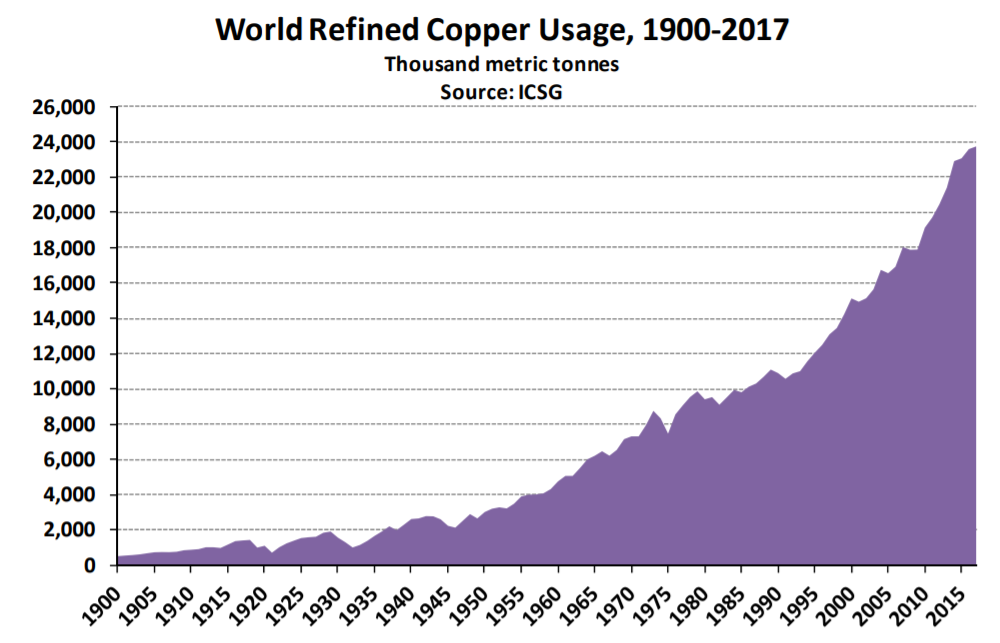
\includegraphics[width=0.8\textwidth]{1/figures/world_refined_copper_usage.png}
%			\caption{Uso del cobre refinado mundial del año 1900 a 2017 (en miles de toneladas). Fuente: \cite{cu_internationalcopper2018}}
%			\label{1:fig}
%		\end{center}
%	\end{figure}
%	}
%	
%	A lo largo de los años, como se observa en la Figura \ref{1:fig}, el uso del cobre refinado (cobre de alta pureza con una concentración de 99.9\%) en el mundo ha tenido un incremento bastante significativo y ello ha conllevado a un aumento en la comercialización de dicho metal. Como consecuencia, este ha contribuido en gran medida para las economías de diversas naciones ya sean países maduros o en vías de desarrollo. El minado, procesamiento, reciclaje y transformación de este metal a varios productos ha creado trabajos y generado riqueza. Estas actividades contribuyen en construir y mantener la infraestructura de un país, y además crea oportunidades de comercio e inversión \parencite{cu_internationalcopper2018}.
%	
%	
%	
%	\begin{figure}[h]
%		\begin{center}
%			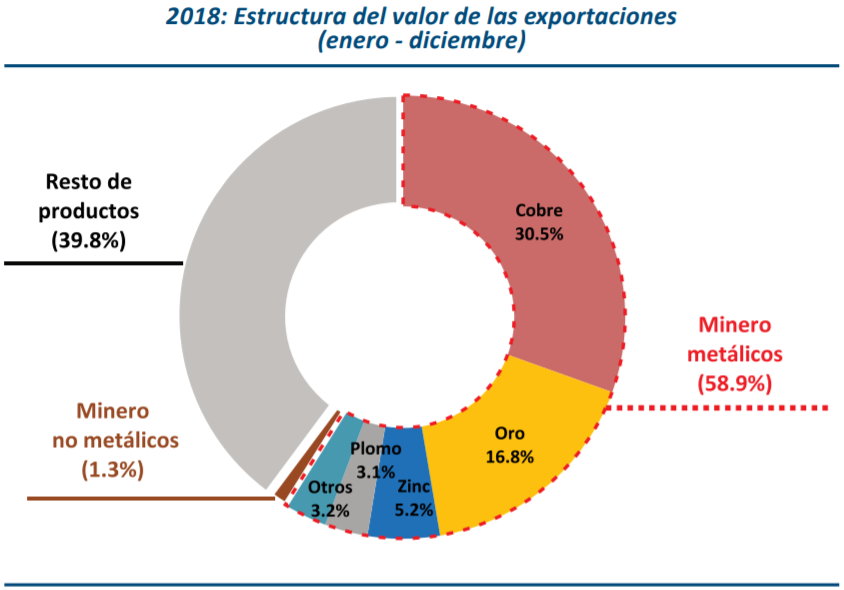
\includegraphics[width=0.8\textwidth]{1/figures/estructura_exportaciones_peru.png}
%			\caption{Estructura del valor de las exportaciones peruanas en el año 2018. Fuente: \cite{cu_ministerioPeru_statsminas}}
%			\label{1:fig2}
%		\end{center}
%	\end{figure}
%	
%	
%	
%	
%	\begin{figure}[h]
%		\begin{center}
%			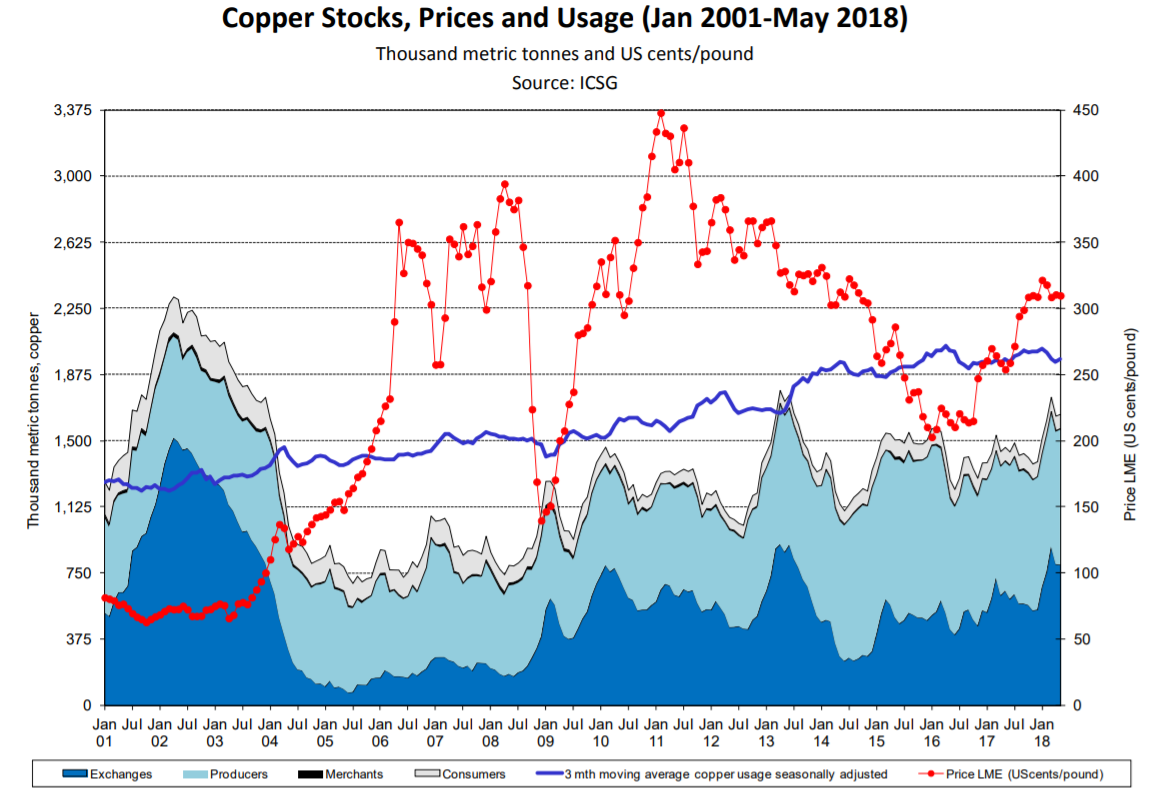
\includegraphics[width=0.8\textwidth]{1/figures/copper_stocks_prices_usage.png}
%			\caption{Precio, stocks y uso del cobre (cantidad en miles de toneladas y precio en centavos por libra). Fuente: \cite{cu_internationalcopper2018}}	
%			\label{1:fig3}
%		\end{center}
%	\end{figure}
%	
%	Estos modelos usados para predecir precios se basan mayormente en estimaciones de la oferta y demanda futura, así como los inventarios de bolsa. Otros consideran la memoria histórica de estas variables, la información de costos futuros de proyectos mineros, o variables financieras. Sin embargo, lo que estos modelos no hacen, es predecir el momento de la caída o alza del precio debido a eventos que no dependen de ninguna de las variables antes mencionadas sino a hechos inesperados globales \citep{cu_lagos2017proyectar}. 
%	
%	
%	\begin{figure}[h]
%		\begin{center}
%			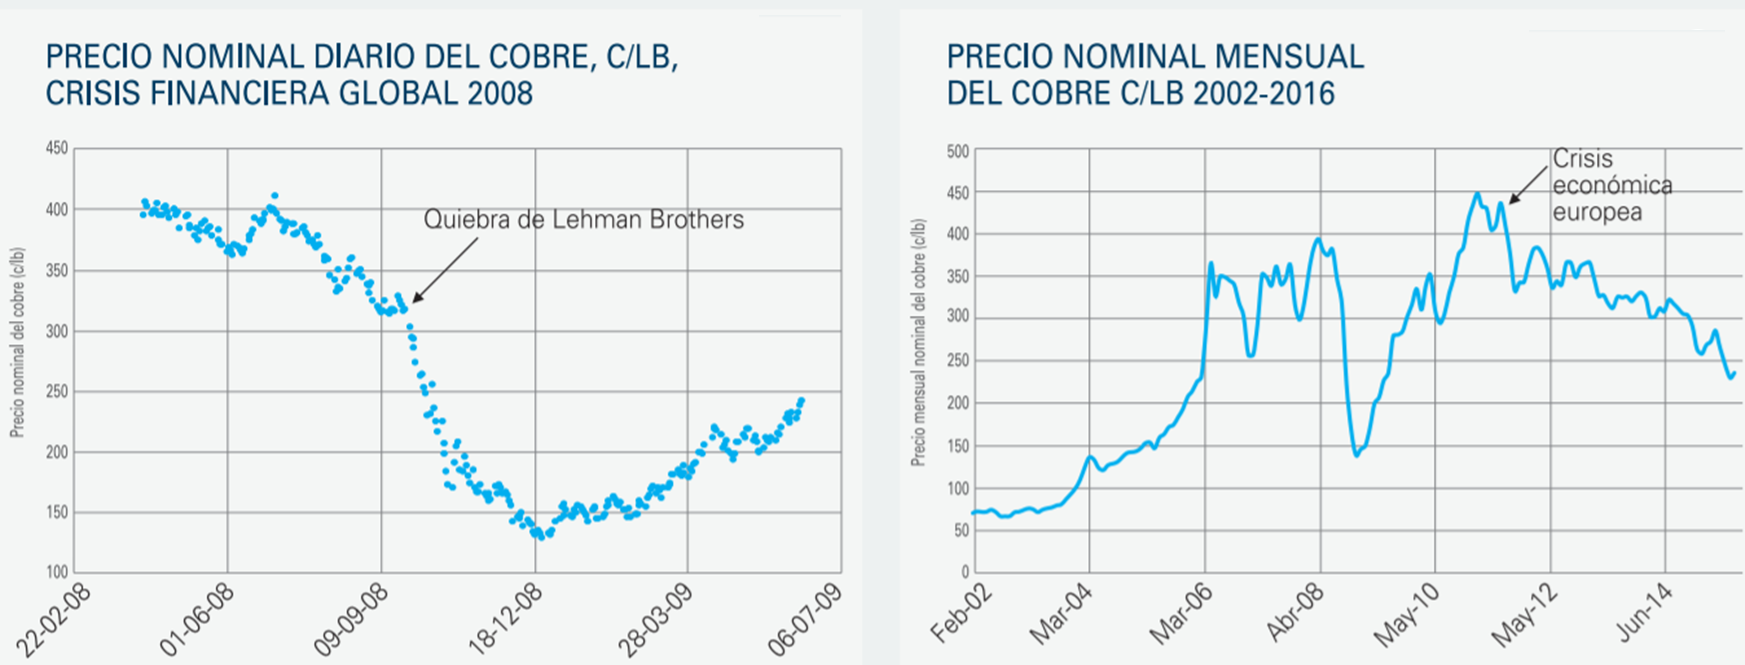
\includegraphics[width=0.8\textwidth]{1/figures/precio_caidas_gustavo_lagos.png}
%			\caption{Precio, stocks y uso del cobre (cantidad en miles de toneladas y precio en centavos por libra). Fuente: \cite{cu_lagos2017proyectar}}
%			\label{1:fig4}
%		\end{center}
%	\end{figure} 




\section{Formulación del Problema}

%Para lefecto \parencite{ot_marti2018manual}. 
%
%
%Una vez elaborado el diagrama (véase Anexo 1), 

\subsection{Problema General}
\newcommand{\ProblemaGeneral}{
	¿Como la implementación de un modelo predictivo de la demanda de productos perecibles beneficiará la toma de decisiones en el proceso del pedido a los proveedores en la empresa Donna SAC?  
}
\ProblemaGeneral
\subsection{Problemas Espec\'{i}ficos}
\newcommand{\Pbone}{
¿Cómo pueden los modelos de predicción de demanda contribuir a una planificación de existencias de productos?
}
\newcommand{\Pbtwo}{
¿Qué técnicas de preprocesamiento de datos son más efectivas para mejorar la precisión de los modelos de predicción de demanda en productos perecibles?
}
\newcommand{\Pbthree}{
¿Cuál es la influencia de las variables de la demanda para predecir productos perecibles y como pueden ajustarse en función al modelo?
}
\newcommand{\Pbfour}{
¿Cuál es la función de los modelos avanzados de Forecasting de la demanda y cómo se comparan con otros métodos de aprendizaje automático en cuanto a precisión y aplicabilidad?
}
%\newcommand{\Pbfive}{
%A
%}

\begin{itemize}
	\item \Pbone
	\item \Pbtwo
	\item \Pbthree
	\item \Pbfour
%	\item \Pbfive
\end{itemize}

\section{Objetivos de la Investigación}
%Para la formulación de los objetivos de la presente investigación se elaboró un «árbol de objetivos» (véase Anexo 2) 
\subsection{Objetivo General}
\newcommand{\ObjetivoGeneral}{
Implementar un modelo predictivo de la demanda de productos perecibles que beneficie la toma de decisiones en el proceso del pedido a los proveedores en la empresa Donna SAC.
}
\ObjetivoGeneral
\subsection{Objetivos Espec\'{i}ficos}
\newcommand{\Objone}{
Determinar cómo los modelos de predicción de demanda pueden contribuir a optimizar la planificación de existencias de productos.
}
\newcommand{\Objtwo}{
Determinar las técnicas de preprocesamiento de datos más efectivas para mejorar la precisión de los modelos de predicción de demanda en productos perecibles. 
}
\newcommand{\Objthree}{
Determinar que variables de la demanda influyen en predecir productos perecibles. 
}
\newcommand{\Objfour}{
Evaluar la eficacia de los modelos avanzados de Forecasting en la predicción de la demanda en una tienda, comparándolos con otros métodos de aprendizaje automático en términos de precisión y aplicabilidad
}
%\newcommand{\Objfive}{
%ghhhg
%}

\begin{itemize}
	\item {\Objone}
	\item {\Objtwo}
	\item {\Objthree}
	\item {\Objfour}
%	\item {\Objfive}
\end{itemize}

\section{Justificación de la Investigación}

\subsection{Teórica}
Se justifica teóricamente primeramente porque las técnicas de aprendizaje automático pueden analizar conjuntos de datos más grandes con mayor eficiencia y precisión que los métodos convencionales, lo que posibilita proporcionar un entendimiento aún más profundo de los patrones y tendencias. Este estudio tiene como propósito aportar nuevos conocimientos en el big data de datos mediante la implementación de técnicas avanzadas de forecasting de series de tiempo. El resultado satisfactorio de este enfoque está destinado a ser utilizado en la gestión precisa de la demanda de productos en el sector minorista, contribuyendo así a la optimización de procesos y la toma de decisiones estratégicas. En conjunto, se busca la eficacia global de la gestión de inventario en el ámbito de la minería de datos. 

\subsection{Práctica}
Esta investigación surge en respuesta a la imperante necesidad de optimizar el aprovechamiento de la valiosa base de datos de nuestra empresa. Nos proponemos no solo hacer uso de los datos históricos disponibles, sino también desarrollar e implementar un modelo predictivo eficiente. El propósito primordial es transformar estos pronósticos en herramientas esenciales para respaldar decisiones estratégicas informadas en la gestión de abastecimiento para nuestras tiendas minoristas. Resaltando esta justificación práctica, buscamos mejorar el desempeño y la eficacia de las operaciones mediante una gestión avanzada de la demanda, lo que a su vez impactará positivamente en la satisfacción del cliente, la optimización de inventarios y la rentabilidad general de la empresa.

\subsection{Metodológica}. 
 El principal problema que ayudará a resolver esta investigación es optimizar la precisión de la predicción de la demanda en las tiendas minoristas. Para ello, se implementará la técnica de forecasting aplicada a las series temporales, buscando obtener la mayor precisión posible en las predicciones de demanda. Este enfoque permitirá una gestión más eficaz del inventario y respaldará decisiones estratégicas basadas en datos predictivos más precisos y actualizados. \\
 La metodología incluirá:
 
 \newcommand{\Mone}{
 	Recopilación de datos históricos de ventas de productos perecibles.}
 \newcommand{\Mtwo}{
 	Identificación y recopilación de variables externas relevantes que puedan influir en la demanda (por ejemplo, eventos especiales, condiciones climáticas, tendencias de mercado). 
 }
 \newcommand{\Mthree}{
 	Selección y aplicación de técnicas de modelado predictivo, como regresión lineal, series temporales, o técnicas más avanzadas como modelos de redes neuronales o machine learning. 
 }
 \newcommand{\Mfour}{
 	Validación del modelo utilizando técnicas como la validación cruzada y la comparación de los resultados predichos con los datos reales de ventas.
 	}
 \newcommand{\Mfive}{
 	Implementación del modelo en un entorno empresarial y evaluación de su impacto en la rentabilidad.
 	}
 
 \begin{itemize}
 	\item {\Mone}
 	\item {\Mtwo}
 	\item {\Mthree}
 	\item {\Mfour}
 	\item {\Mfive}
 \end{itemize}

\section{Delimitación del Estudio}

\subsection{Espacial}
Se realizará en la empresa Donna S.A.C. ubicada en el distrito de Breña, Provincia y Departamento de Lima. Teniendo como giro principal la venta de productos de supermercado. 

\subsection{Temporal}
Se llevará a cabo en la empresa Donna S.A.C. mediante el análisis de los datos mensuales obtenidos desde el año 2023 al 2024, los cuales se obtendrán a partir de la data registrada por la empresa y proporcionados por el personal encargado del manejo de datos. 

\subsection{Conceptual}
La presente, realizada en la empresa Donna S.A.C., se enfoca en la implementación de un modelo de Series de tiempo basado en algoritmos de aprendizaje automático. Este enfoque nos ayudará a realizar predicciones en la empresa, y la implementación se llevará a cabo utilizando herramientas básicas de producción. Se establecerán relaciones entre las diversas áreas presentes dentro de la empresa. Se evaluarán los beneficios que atraerá dicha implementación y se buscarán maneras de continuar mejorando el proceso.

\section{Hipótesis}

\subsection{Hipótesis General}
\newcommand{\HipotesisGeneral}{
La implementación de un modelo predictivo de la demanda de productos perecibles beneficiara en la toma de decisiones en el proceso de pedido a los proveedores en la empresa Donna SAC.
}
\HipotesisGeneral
\subsection{Hipótesis Específicas}
\newcommand{\Hone}{
El uso de modelos de predicción de demanda mejora la planificación de existencias de productos asegurando la disponibilidad adecuada.
}
\newcommand{\Htwo}{
Las técnicas de procesamiento de datos como la normalización de datos, el tratamiento de valores atípicos y la selección de características relevantes, serán más efectivas para mejorar la precisión de los modelos de predicción de demanda en productos perecibles  
}
\newcommand{\Hthree}{
 Las variables escogidas de la demanda tienen influencia significativa en el modelo.
}
\newcommand{\Hfour}{
Los modelos avanzados de Forecasting proporcionan una mayor precisión y aplicabilidad en la predicción de la demanda en un entorno de tienda, en comparación con otros métodos de aprendizaje automático
}
%\newcommand{\Hfive}{
%	xws
%}
\begin{itemize}
	\item \Hone
	\item \Htwo
	\item \Hthree
	\item \Hfour
%	\item \Hfive
\end{itemize}

\subsection{Matriz de Consistencia}
A continuación se presenta la matriz de consistencia elaborada para la presente investigación (véase Anexo \ref{1:table}).


\include{2/marco}
\chapter{ENTORNO EMPRESARIAL}

\section{Descripción de la empresa}
\subsection{Reseña histórica y actividad económica}
Donna S.A.C, una exitosa empresa dedicada a los minimercados, se ha establecido como un destino de compras esencial para la comunidad. Con cuatro ubicaciones estratégicas, esta cadena se ha convertido en un punto de referencia para aquellos que buscan productos de calidad y atención personalizada. Su lema, "Donna S.A.C, donde cada compra es una experiencia", refleja su compromiso con la creación de un ambiente cálido y acogedor para sus clientes. Desde la entrada, los clientes son recibidos con un diseño moderno y limpio, facilitando una experiencia de compra placentera. La atención al cliente es primordial, con empleados capacitados siempre dispuestos a brindar ayuda, garantizando que cada visita sea positiva.
\newline

Las cuatro tiendas de Donna S.A.C están estratégicamente ubicadas para ofrecer fácil acceso a una amplia gama de productos, desde alimentos frescos hasta artículos para el hogar, satisfaciendo las cambiantes necesidades de sus clientes. Con un equipo de veinte empleados comprometidos, Donna S.A.C ha cultivado un ambiente laboral colaborativo y motivador mediante una capacitación continua que asegura un servicio informado y útil para los clientes. Esta dedicación al desarrollo del equipo no solo beneficia a los empleados, sino que también contribuye al ambiente positivo que caracteriza a cada tienda.

\subsection{Descripción de la organización}

% Descripción de Donna S.A.C: Más Allá de un Minimarket, una Experiencia de Compra Inigualable.
% \newline

Donna S.A.C, una cadena de minimarkets que va más allá de las expectativas convencionales, ha dejado una marca distintiva en el mundo de las compras minoristas. Con cuatro ubicaciones estratégicas, esta empresa se ha convertido en un pilar esencial para aquellos que buscan no solo productos de elevada calidad, así mismo una experiencia de compra inigualable.
\newline

Cada tienda Donna S.A.C ha sido diseñada con esmero para crear un ambiente acogedor y moderno. Desde la entrada, los clientes son recibidos con un diseño limpio y una disposición intuitiva de productos. La tienda no es solo un espacio de transacciones; es un destino donde la atención al cliente es una prioridad. Nuestro equipo de veinte empleados capacitados está siempre disponible para ayudar, proporcionando un servicio personalizado que transforma cada visita en una experiencia positiva.
La diversidad de productos en Donna Sac es impresionante, desde alimentos frescos y productos del hogar hasta opciones de conveniencia para satisfacer las necesidades diarias. La cadena se enorgullece de mantener sus estantes abastecidos con productos de alta calidad, ofreciendo a los clientes la confianza de que encontrarán lo que necesitan, cuando lo necesiten.
\newline

Detrás de la exitosa operación de Donna Sac se encuentra un equipo de veinte trabajadores dedicados que personifican los valores de la empresa. La capacitación frecuente y el desarrollo profesional son fundamentales para nuestro enfoque en el servicio al cliente, asegurando que cada miembro del equipo esté bien informado y preparado para brindar asesoramiento útil.

\subsubsection{Organigrama}
Este organigrama es una representación simplificada de la estructura jerárquica de Donna Sac. Cada posición puede tener roles específicos y responsabilidades detalladas, y la organización está diseñada para fomentar la eficiencia operativa, la atención al cliente excepcional y la participación comunitaria.

\begin{figure}[h]
	\begin{center}
			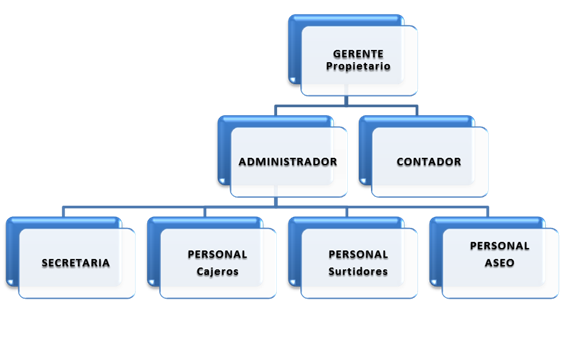
\includegraphics[width=0.8\textwidth]{31/figures/organigrama.png}
			\caption{Organigrama Donna SAC}
			\label{fig1}
	\end{center}			
\end{figure}

\subsection{Datos generales estratégicos de la empresa}
Información Básica:

\begin{itemize}
		\item Nombre completo de la empresa: Donna Sac.
		\item Fecha de fundación: 2000.
		\item Fundadores o actuales propietarios: Donaciano Paucar. 
		\item Tiendas: 6 tiendas.
		\item Ubicación de cada tienda: 2 en Chorrillos, Surco, 2 en La Molina, Breña.
		\item Tamaño promedio de las tiendas en pies cuadrados: 120 ft$^2$
		\item Número total de empleados: 40.
		\item Productos y Servicios: Consumo masivo.
		\item Segmentos de mercado objetivo: Personas proximas a las tiendas de Donna SAC.
\end{itemize}

\subsubsection{Visión, misión y valores o principios}
\textbf{Visión:} ``Ser reconocidos como el referente líder en la experiencia de compra minorista, destacando por nuestra dedicación excepcional al cliente, la innovación en productos y servicios, y nuestro impacto positivo en las comunidades que servimos."
\newline

\textbf{Misión:} ``En Donna Sac, nos comprometemos a ofrecer a nuestros clientes una experiencia de compra única y satisfactoria, brindando productos de alta calidad, un servicio personalizado y contribuyendo activamente al bienestar de las comunidades locales. Nos esforzamos por ser un destino esencial para aquellos que buscan más que una simple transacción, buscando una conexión significativa con sus necesidades diarias y valores compartidos."

\subsubsection{Objetivos estratégicos}
\textbf{Excelencia en la Experiencia del Cliente:}
\begin{itemize}
	\item Mejorar continuamente la atención al cliente para garantizar una experiencia de compra excepcional.
	\item Implementar programas de capacitación para el equipo humano que refuercen la significación del servicio al cliente.
\end{itemize}

\textbf{Diversificación y Ampliación de Productos:}
\begin{itemize}
	\item Investigar y agregar nuevos productos que satisfagan las tendencias del mercado y las necesidades cambiantes de los clientes.
	\item Expandir las líneas de productos propios para aumentar la diferenciación en el mercado.
\end{itemize}

\textbf{Innovación en Tecnología y Operaciones:}
\begin{itemize}
	\item Implementar tecnologías avanzadas para mejorar la eficiencia operativa, desde sistemas de gestión de inventario hasta soluciones de punto de venta.
	\item Explorar oportunidades para la implementación de plataformas digitales que mejoren la experiencia del cliente y faciliten la expansión en línea.
\end{itemize}

\textbf{Desarrollo de la Cadena de Suministro Sostenible:}
\begin{itemize}
	\item Contribuir con proveedores implicados con prácticas sostenibles y éticas.
	\item Reducir la huella ambiental mediante prácticas de gestión de residuos y opciones de embalaje sostenibles.
\end{itemize}

\textbf{Expansión Geográfica y Nuevas Tiendas:}
\begin{itemize}
	\item Identificar y evaluar nuevas ubicaciones estratégicas para la apertura de tiendas.
	\item Establecer alianzas con desarrolladores inmobiliarios para facilitar la expansión.
	\item Iniciativas de Responsabilidad Social Corporativa.
	\item Introducir iniciativas de responsabilidad social corporativa  
	\item Establecer asociaciones con organizaciones benéficas y participar activamente en eventos comunitarios.
\end{itemize}

\textbf{Optimización Financiera:}
\begin{itemize}
	\item Mejorar la eficiencia financiera mediante la implementación de herramientas de análisis y seguimiento.
	\item Buscar oportunidades para mejorar los márgenes de beneficio sin afectar la calidad de los recursos y servicios.
\end{itemize}

\subsubsection{Evaluación interna y externa. FODA}


	
%%%%%%%%%%%%%%%%%%%%%%%%%%%%%%

\begin{longtable}{L{5cm} | C{2.5cm} | C{2.5cm} | C{2.5cm} }
	\hline
	%\rowcolor{Gainsboro!60}
	\rowcolor{Gray}
	\makecell{Oportunidades} & \makecell{Ponderación}  & \makecell{Clasificación} & \makecell{Puntuación}\\
	\hline
	\endhead
	El crecimiento de la clase	media peruana está generando una mayor demanda de productos y servicios de calidad. La tendencia de los peruanos se está centrando en la obtención de productos de manera más rápida y en menores	tiempos de espera. & 0.3 & 3 &0.90\\
	\hline
	El cambio en los hábitos de consumo, los nuevos consumidores buscan cuidar su salud por lo que buscan frutas al momento de entrar a una tienda minorista. & 0.05 & 3 & 0.15\\
	\hline
	Cada vez salen nuevas marcas de productos de consumo masivo al mercado. Las alianzas estratégicas con otras empresas podrían ayudar a Donna a ampliar su oferta de productos. & 0.1 & 2 & 0.20\\
	\hline
	La innovación tecnológica podría ayudar a Donna  a mejorar la eficiencia y la experiencia de compra de los clientes. Implementación de IA en la capacitación o cajeros automáticos. & 0.05 & 2 & 0.10\\
	\hline
	Las inversiones en marketing podrían ayudar a Donna el aumentar su reconocimiento de marca y atraer a nuevos clientes. Expansión de sus redes sociales y crear campañas que se alineen con las nuevas tendencias en su público objetivo. & 0.15 & 1 & 0.15\\
	\hline
	 & 0.65 &  & 1.50\\
	\hline
	\caption{Oportunidades de Donna Sac}
	\label{tab:widgets}
\end{longtable}

%%AMENAZAS

\begin{longtable}{L{5cm} | C{2.5cm} | C{2.5cm} | C{2.5cm} }
	\hline
	%\rowcolor{Gainsboro!60}
	\rowcolor{Gray}
	\makecell{Amenazas} & \makecell{Ponderación}  & \makecell{Clasificación} & \makecell{Puntuación}\\
	\hline
	\endhead
	El crecimiento del sector de las tiendas minoristas está generando una mayor competencia. & 0.15 & 2 &0.30\\
	\hline
	Los cambios en la inestabilidad económica y cambios de gobierno reducen el tiempo de compra de productos. Muchos consumidores obtan por las tiendas mayoristas en este tipo de situaciones. & 0.05 & 2 & 0.10\\
	\hline
	Tambo posee una participación del 30\% en la categoria de tiendas minoristas. & 0.05 & 2 & 0.10\\
	\hline
	Los cambios en los hábitos de consumo, hacia una mayor orientación hacia los productos orgánicos o saludables, podrían afectar la demanda de los productos de Donna y replantear un nuevo stock de productos. & 0.05 & 3 & 0.15\\
	\hline
	Problemas de politica exterior de Perú con países a los que compramos productos internacionales podrian afectar el precio compra al que llegan a nuestro país. & 0.05 & 2 & 0.10\\
	\hline
	& 0.35 &  & 0.75\\
	\hline
	\caption{Amenazas de Donna Sac}
	\label{tab:widgets}
\end{longtable}

La empresa Donna se encuentra por debajo del promedio en cuestión de respuesta a los factores exteriores. Se recomienda darle más importancia a lo que esta pasando en su entorno macro para poder aprovechar las oportunidades del mercado.

\begin{longtable}{L{5cm} | C{2.5cm} | C{2.5cm} | C{2.5cm} }
	\hline
	%\rowcolor{Gainsboro!60}
	\rowcolor{Gray}
	\makecell{Fortalezas} & \makecell{Ponderación}  & \makecell{Clasificación} & \makecell{Puntuación}\\
	\hline
	\endhead
	Experiencia de 20 años en el mercado minorista, conocimientos del entorno y adaptación a los diversos escenarios del proceso de compra del consumidor. & 0.20 & 4 &0.80\\
	\hline
	Ofrece productos mucho más variados que otras tiendas minoristas que estan top en la categoría, Donna ofrece productos que abarcan hasta frutas y verduras que son del día. & 0.10 & 4 & 0.40\\
	\hline
	Donna se ubica en zonas de alto tráfico peatonal, lo que facilita el acceso a nuevos clientes & 0.05 & 3 & 0.15\\
	\hline
	Se ofrece una pequeña capacitación de unos 3 días al personal para que se enfoque en crear relación con el cliente y que no solo se convierta en una transacción de bienes. Se le proporciona videos y un taller que se enfoca en ser empatico con el cliente al preguntar cosas de su vida diaria. & 0.15 & 4 & 0.60\\
	\hline
	Empleados jóvenes, más agiles y que recomiendan productos a los clientes con mayor rapidez de acuerdo a las tendencias del mercado. & 0.10 & 3 & 0.30\\
	\hline
	& 0.60 &  & 2.25\\
	\hline
	\caption{Fortalezas de Donna Sac}
	\label{tab:widgets}
\end{longtable}

%%%%%DEBILIDADES

\begin{longtable}{L{5cm} | C{2.5cm} | C{2.5cm} | C{2.5cm} }
	\hline
	%\rowcolor{Gainsboro!60}
	\rowcolor{Gray}
	\makecell{Debilidades} & \makecell{Ponderación}  & \makecell{Clasificación} & \makecell{Puntuación}\\
	\hline
	\endhead
	La mayoría de las tiendas de Donna se encuentran en zonas urbanas, lo que limita su alcance al mercado rural. & 0.15 & 1 &0.15\\
	\hline
	Donna tiene una marca poco diferenciada, lo que puede dificultar su posicionamiento frente a la competencia que son en su mayoría tiendas de esquina o los mismos mercados. & 0.05 & 1 & 0.05\\
	\hline
	Donna se concentra en la venta de productos básicos, lo que limita su oferta de productos a un público más especializado. & 0.05 & 2 & 0.10\\
	\hline
	Donna no posee un horario de atención de 24 horas. & 0.10 & 1 & 0.10\\
	\hline
	Alta rotación de personal, no se crea identidad de marca con el personal interno. & 0.05 & 2 & 0.10\\
	\hline
	& 0.40 &  & 0.50\\
	\hline
	\caption{Debilidades de Donna Sac}
	\label{tab:widgets}
\end{longtable}


\begin{figure}[H]
	\begin{center}
		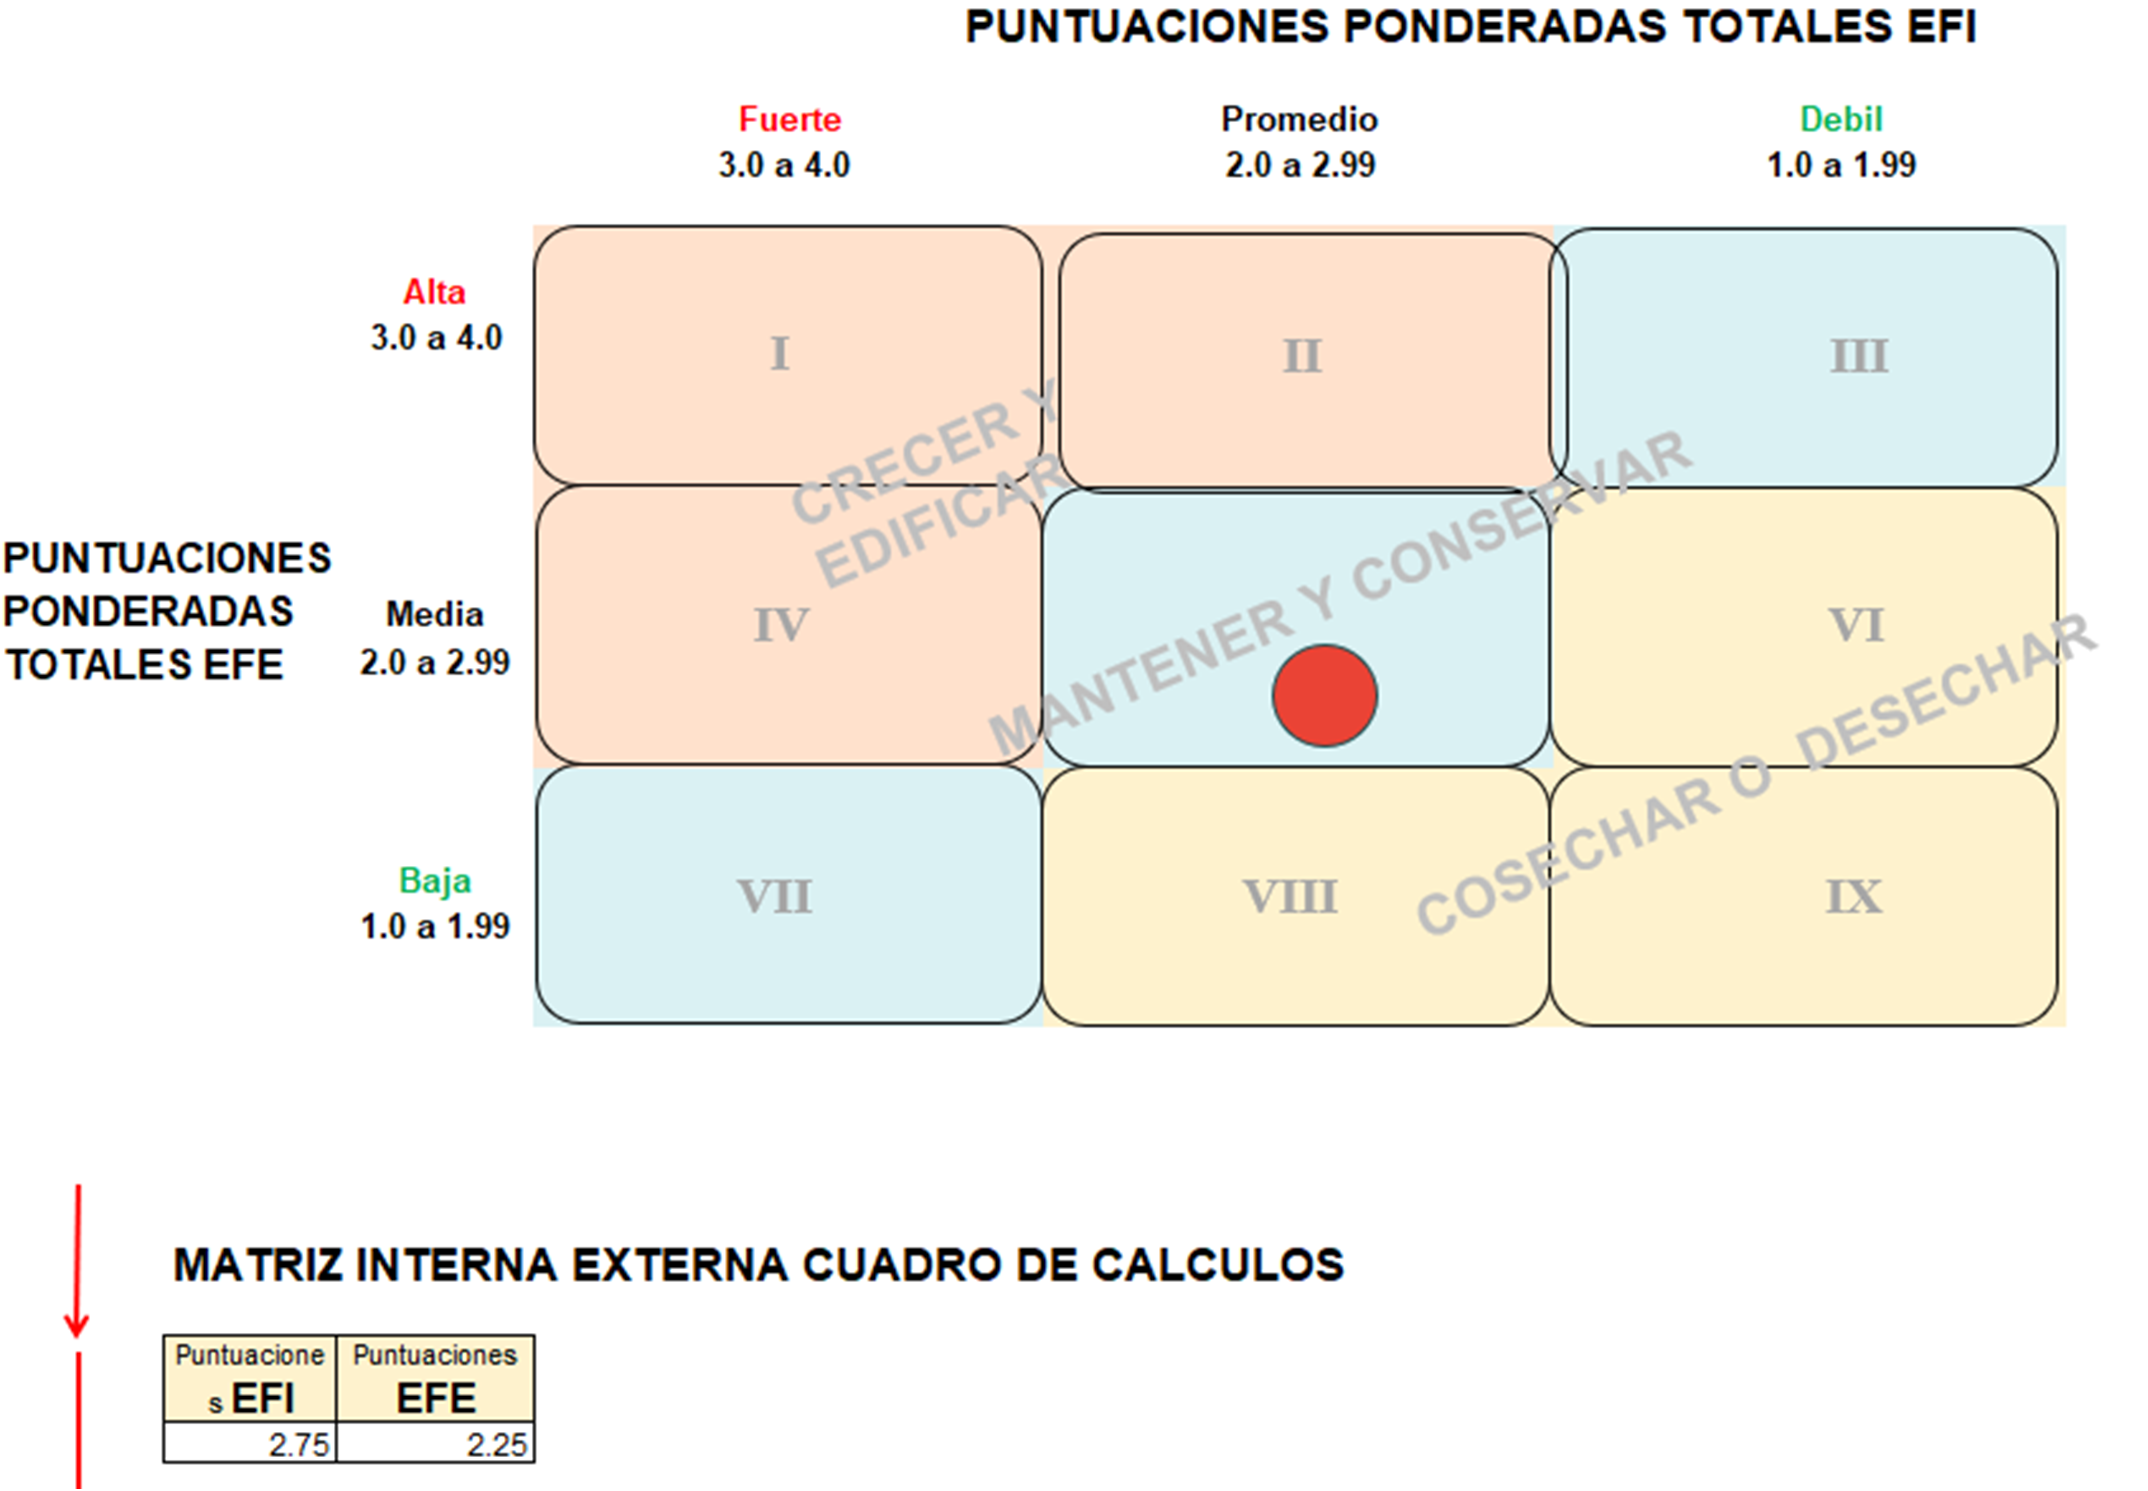
\includegraphics[width=0.8\textwidth]{31/figures/Matriz_EFI_EFE.png}
		\caption{Matriz interna y externa}
		\label{fig31.1}
	\end{center}			
\end{figure}

Donna se encuentra en la Celda V, por lo tanto le conviene la estrategia de mantener y conservar.  Lo que se plantea que haga Donna al no ser una opción la penetración de mercado por razones económicos es optar por la estrategia de desarrollo de producto. Lo que se plantea es introducir nuevos productos orgánicos y saludables, debido a la demanda de salud que está en crecimiento. Además, mejorar la calidad de productos y priorizar el bienestar del consumidor, darle un extra a cada compra para que pueda recordar nuestra marca.


\subsection{Modelo de negocio actual (CANVAS)}

\begin{figure}[H]
	\begin{center}
		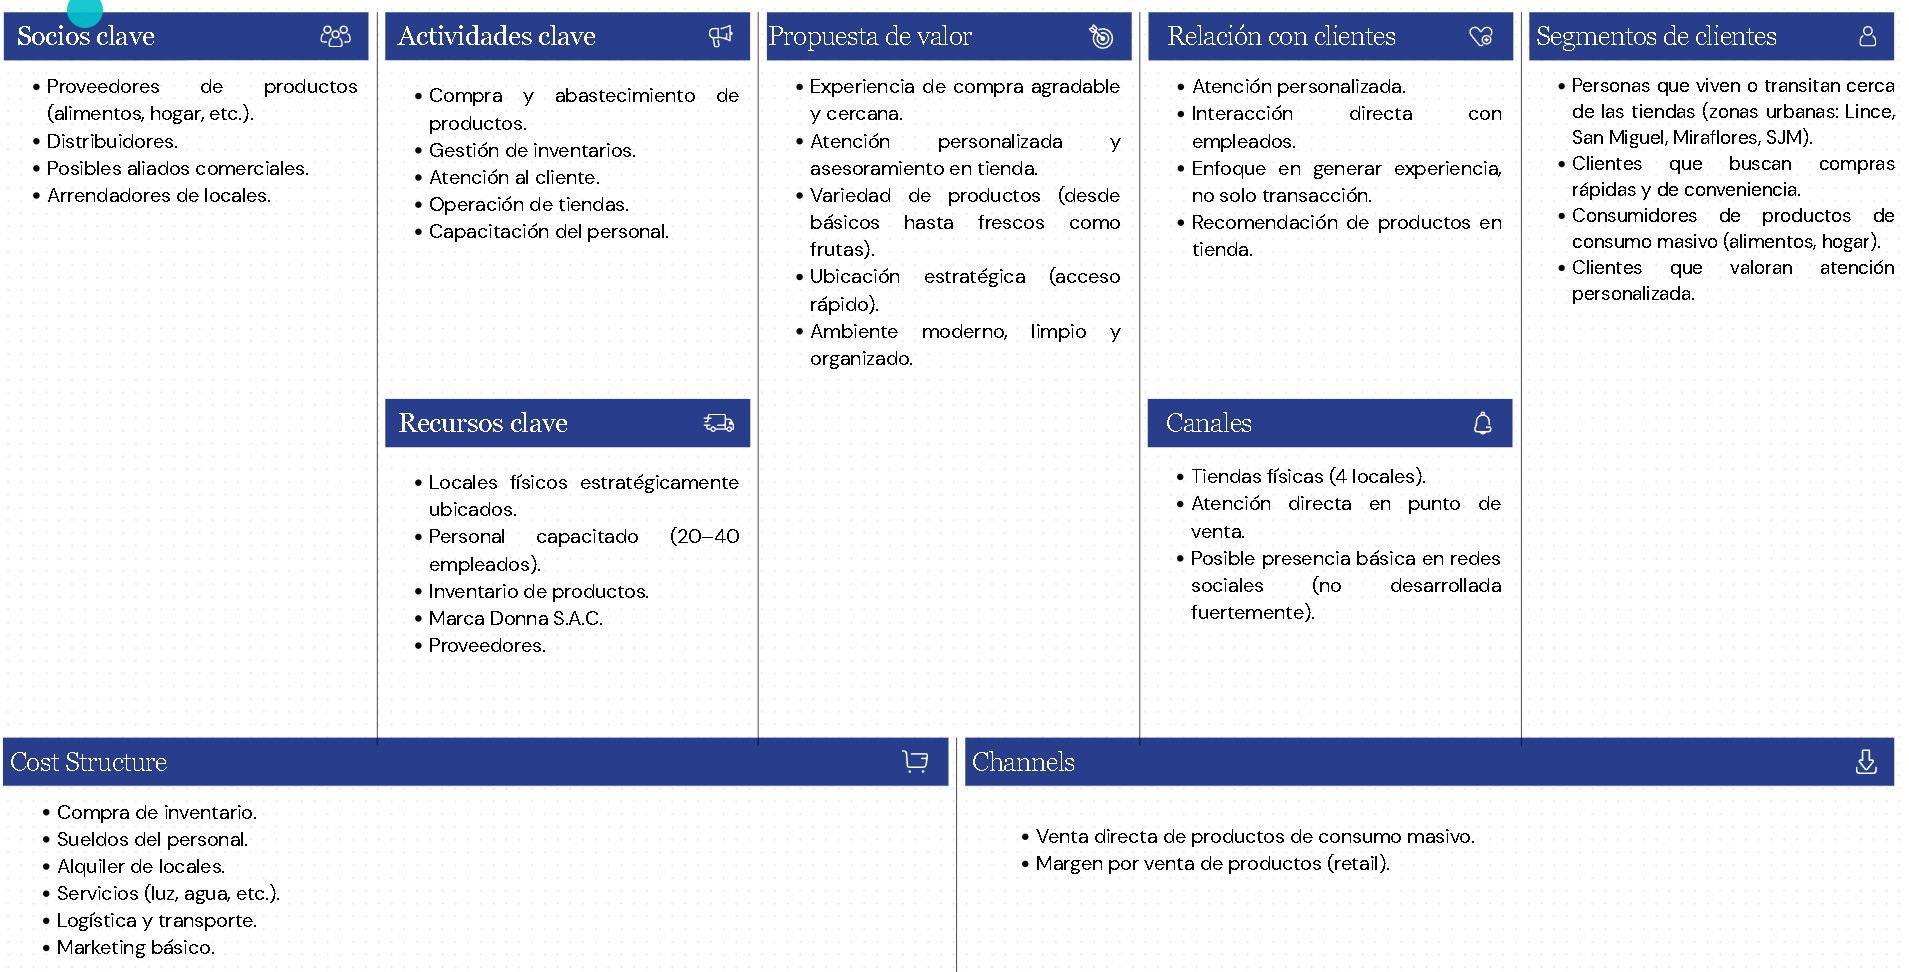
\includegraphics[width=0.9\textwidth]{31/figures/B CANVAS.JPG}
		\caption{Business Model Canvas}
		\label{fig31.2}
	\end{center}			
\end{figure}


% \subsection{Mapa de procesos actual}	



%\begin{longtable}{L{4cm} | C{2cm} | C{1.9cm} | C{1.9cm} | C{1.9cm} | C{1.9cm}| C{1.9cm}| C{1.9cm} }
%	\hline
%	%\rowcolor{Gainsboro!60}
%	\rowcolor{Gray}
%	\makecell{} & \makecell{} & \makecell{PERU} & \makecell{} & \makecell{COLOMBIA} & \makecell{} & \makecell{BRASIL}\\
%	\hline
%	\endhead
%		\makecell{Factores para el éxito} & \makecell{Ponderación}  & \makecell{Calificación} & \makecell{Puntuación} & \makecell{Calificación} & \makecell{Puntuación} & \makecell{Calificación} & \makecell{Puntuación}\\
%	\hline
%	
%	Crecimiento económico & 0.15 & 1 &0.15\\
%	\hline
%	Uso de Data Mining & 0.05 & 1 & 0.05\\
%	\hline
%	Expansión empresarial & 0.05 & 2 & 0.10\\
%	\hline
%	Desafíos en la gestión de inventarios & 0.10 & 1 & 0.10\\
%	\hline
%	Beneficios de la implementación de modelos predictivos & 0.05 & 2 & 0.10\\
%	\hline
%	Adopción de tecnologías emergentes & 0.40 &  & 0.50\\
%	\hline
%	Infraestructura logística & & & &\\
%	\hline
%	Participación en acuerdos comerciales & & & &\\
%	\hline
%	\caption{Debilidades de Donna Sac}
%	\label{tab:widgets}
%\end{longtable}





\chapter{METODOLOGÍA DE LA INVESTIGACIÓN}
\section{Diseño de la investigación}
En esta sección del documento se explicará cual es el diseño, el tipo y el enfoque del trabajo de investigación, así como también la población y la muestra del estudio. 
%Para finalizar se explicará el
%proceso de aplicación de las redes neuronales convolucionales.
\subsection{Enfoque}
Esta investigación adopta un enfoque cuantitativo, centrado principalmente en el análisis de datos históricos y la aplicación de modelos de series temporales para abordar la demanda de productos perecibles. La metodología se basa en la recopilación y análisis de datos cuantitativos diarios relacionados con la demanda, con el objetivo de ofrecer información y recomendaciones basadas en rigor estadístico y en la interpretación de patrones numéricos. Esto permitirá optimizar la gestión de la demanda de productos y mejorar la eficiencia operativa en la toma de decisiones de inversión en los pedidos a proveedores.

\subsection{Alcance}
Esta investigación es de tipo explicativa, ya que busca identificar los componentes y parámetros específicos que afectan la eficiencia de la cadena de suministro de la empresa Market Donna SAC. En particular, se centrará en el desarrollo e implementación de un sistema de pronóstico de demanda basado en modelos de Forecasting. El alcance se extiende a la evaluación del impacto de este sistema en la gestión de las órdenes de productos perecibles, analizando los beneficios en términos de optimización de inversión, reducción de costos y mejora de la eficiencia operativa.

\subsection{Tipo}
La investigación es de tipo no experimental, dado que se trabajará con datos históricos comprendidos entre el año 2012 Y 2026. A partir de este análisis, se desarrollará un modelo predictivo para mejorar la precisión en la estimación de la demanda de productos en Market Donna SAC y, así, orientar decisiones más efectivas. 

%\subsection{Enfoque cuantitativo}




%%%%%%%%%%%%%%%%%%%%%%%%%%%%%%%%%%%

\subsection{Población y muestra}

La población de estudio incluye todas las categorías de productos que Market Donna SAC ofrece, entre las cuales se encuentran artículos de limpieza, frutas, verduras, lácteos, carnes, bebidas, abarrotes, tabaco, condimentos, embutidos, panes, entre otros. En total, la empresa cuenta con 16 categorías de productos que generan un promedio de 136,000 soles mensuales en ventas.
La muestra seleccionada se concentra específicamente en la categoría de Verduras, que representa una de las familias de productos con mayor impacto en las ventas de la empresa. Al centrarnos en esta categoría de productos perecibles, el estudio busca realizar un análisis más preciso de la demanda diaria y proyectar las ventas en soles para la familia de verduras, dada su relevancia en las operaciones y en la rentabilidad de Market Donna SAC.


\subsection{Unidad de análisis}
La unidad de análisis de este estudio se centra en cada transacción individual de venta de productos dentro de la categoría seleccionada, que corresponde a las verduras. Cada transacción registrada en este segmento, desde el año 2012 hasta 2026, se considera como una unidad única de observación. Esto permite una comprensión granular y precisa de los patrones de compra, comportamientos de los clientes y tendencias de demanda asociadas específicamente a estos productos perecibles.
Al examinar cada transacción de manera individual, el análisis busca capturar variaciones diarias en la demanda, observar los patrones de consumo recurrentes y detectar posibles picos o caídas en las ventas. Este enfoque detallado proporciona información valiosa para construir un modelo predictivo ajustado a las particularidades de la categoría de verduras, permitiendo identificar factores que podrían influir en la demanda, como la estacionalidad, días de la semana, campañas promocionales o eventos externos.
Además, el análisis de estas transacciones ofrece la oportunidad de estudiar la sensibilidad de la demanda a las variaciones en precios y promociones dentro de esta categoría. Estos datos permitirán una mejor previsión de la demanda en soles y servirán de base para la toma de decisiones estratégicas sobre los volúmenes de compra y la inversión diaria en reposición de inventario, asegurando así la disponibilidad de productos frescos y optimizando la eficiencia operativa de Market Donna SAC en esta categoría de productos perecibles.


%La Figura \ref{fig1} y el Cuadro \ref{tab:widgets}
%
%	\begin{figure}[h]
	%		\begin{center}
		%			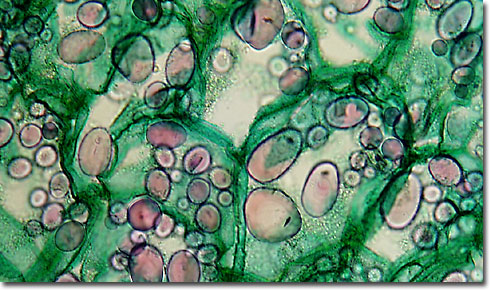
\includegraphics[width=0.8\textwidth]{3/figures/largepotato.jpg}
		%			\caption{Prueba de Figura}
		%			\label{fig1}
		%		\end{center}
	%		
	%	\end{figure}


%\subsection{Operacionalización de Variables}
%
%
%\begin{longtable}{L{2.7cm} | L{4cm} | C{2cm} | C{2.5cm} }
%	\hline
%	\caption{Matriz de operacionalización de variables}
%	%\rowcolor{Gainsboro!60}
%	%\rowcolor{Gray}
%	\makecell{Variable} & \makecell{Definición \\ operacional}  & \makecell{Indicador} & \makecell{Fórmula}\\
%	\hline
%	\endhead
%	Independiente: Optimización en la toma de decisiones & Cantidad óptima de pedidos a realizar a los proveedores, con el fin de minimizar los costos operativos y los desperdicios, al mismo tiempo que se maximiza la disponibilidad de productos y se mejora la eficiencia del inventario  & Cantidad óptima de pedidos & pedido\ proveedor\ <\ demanda\\
%	\hline
%%	Dependiente: Demanda de productos & Cantidad específica de productos que se espera que los consumidores compren en un período de tiempo determinado, basada en datos históricos de ventas & Cantidad de productos & Número de pedidos \le Demanda\\
%%	\hline
%%	\multirow{4}{*}{Modelo \\ de regresión} & \multirow{4}{*}{Modelo con la capacidad de predecir la cantidad aproximada de demanda de productos}  & MSE & \\
%	
%	& & RMSE & \\
%	
%	& & R2 & \\	
%	
%	& & ACCURACY & \\
%	
%	\newline
%	\newline \textit{Fuente: Elaboración propia}
%	\label{tab:widgets}
%\end{longtable}




%%%% TABLA

%\begin{table}[H]
%	\centering
%	\begin{tabular}{|L{2.7cm}|L{4cm}|C{1.9cm}|C{2.5cm}|}
	%		\hline
	%		Variable & Definición operacional & Indicador & Fórmula\\
	%		\hline
	%		Independiente: Optimización en la toma de decisiones & Cantidad óptima de pedidos a realizar a los proveedores, con el fin de minimizar los costos operativos y los desperdicios, al mismo tiempo que se maximiza la disponibilidad de productos y se mejora la eficiencia del inventario & Cantidad óptima de pedidos & Fórmula 1  \\
	%		\hline
	%		Dependiente: Demanda de productos & Cantidad específica de productos que se espera que los consumidores compren en un período de tiempo determinado, basada en datos históricos de ventas & Cantidad de productos & Fórmula 2  \\
	%		\hline
	%		\multirow{3}{*}{Modelo de \\ regresión} & \multirow{3}{4cm}{Modelo con la capacidad de predecir la cantidad aproximada de demanda de productos} & \multirow{2}{*}{Combinadas} & Fórmula 3 \\
	%		\cline{2-2} \cline{4-4}
	%		& & & Fórmula 4 \\
	%		\cline{2-4}
	%		& & Indicador extra & Fórmula 5 \\
	%		\hline
	%	\end{tabular}
%	\caption{Tabla simple}
%\end{table}


%	\begin{table}[ht]
	%	\centering
	%	\begin{tabular}{|c|l|c|r|m{4cm}|}
		%		\hline
		%		Columna 1 & Columna 2 & \multicolumn{2}{c|}{Columna Combinada} & Columna con P\'arrafo\\
		%		\hline
		%		\hline
		%		Fila 1 & Celda 11 & Celda 12 & Celda 13 & Este es un párrafo de muestra en la primera celda de la última columna \\
		%		\hline
		%		\rowcolor{skyblue6}
		%		Fila 2 & Celda 21 & Celda 22 & Celda 23 & Celda P\'arrafo 24 \\
		%		\hline
		%		\parbox[t]{2mm}{\multirow{3}{*}{\rotatebox[origin=c]{90}{Fila 3}}} & Celda 31 & \multirow{2}{*}{Celdas Combinadas} & Celda 33 & Celda P\'arrafo 34  \\
		%		\cline{2-2} \cline{4-5}
		%		& Celda 41 & & Celda 43 & Celda P\'arrafo 44 \\
		%		\cline{2-5}
		%		& Celda 51 & Celda 52 & Celda 53 & Celda P\'arrafo 54  \\
		%		\hline
		%	\end{tabular}
	%	\caption{Tabla simple}
	%\end{table}
	
	%\section{Instrumentos de medida}
	%Nisi porta lorem mollis aliquam ut porttitor leo. Aenean pharetra magna ac placerat \begin{itemize}
		%	\item muscle and fat cells remove glucose from the blood,
		%	\item cells breakdown glucose via glycolysis and the citrate cycle, storing its energy in the form of ATP,
		%	\item liver and muscle store glucose as glycogen as a short-term energy reserve,
		%	\item adipose tissue stores glucose as fat for long-term energy reserve, and
		%	\item cells use glucose for protein synthesis.
		%\end{itemize}
		
		\section{Técnicas de recolección de datos}
		La recolección de datos para esta investigación se focalizó en la obtención de información sobre la categoría de verduras, la cual representa en promedio el 33 \% de la demanda diaria en Market Donna SAC. Esta categoría fue seleccionada estratégicamente debido a su relevancia en la demanda diaria y su corta vida útil, lo que la convierte en un componente esencial para el análisis de productos en la empresa.
		Para implementar el modelo de series de tiempo y realizar pronósticos de demanda diarios que contribuyan a maximizar los ingresos, se llevó a cabo una recopilación exhaustiva de datos históricos a través de un sistema de administración de bases de datos en SQL Server. Inicialmente, se desarrollaron consultas SQL específicas \ref{fig:querysql} para filtrar y extraer las tablas relevantes, tales como las de productos, precios, familias y códigos. Este proceso permitió estructurar y organizar la información de manera adecuada para su posterior análisis.
		Posteriormente, se diseñó una consulta SQL \ref{fig:tablasql} avanzada que integró y combinó las tablas requeridas, garantizando la coherencia e integridad de los datos necesarios para construir los modelos de pronóstico de demanda. Esta metodología proporcionó un conjunto de datos preciso y completo, indispensable para la aplicación de técnicas avanzadas de series de tiempo.
		El análisis incluyó el examen detallado de transacciones de productos de la categoría de verduras desde el año 2012 hasta 2026, brindando una perspectiva temporal amplia para identificar patrones y tendencias de demanda diaria a lo largo del tiempo. Además, se utilizó el sistema de punto de venta (POS) de la empresa para capturar datos en tiempo real sobre las transacciones, lo que permitió un seguimiento constante y detallado de la demanda en esta categoría.
		Para mejorar la precisión de los datos, se revisaron registros continuos de los niveles de inventario de la categoría de verduras. Aunque la investigación se centra en la demanda y no en la gestión de inventarios, este seguimiento indirecto permitió observar cómo la demanda afecta la reposición de productos perecibles, lo cual es crucial para la planificación diaria en productos de alta rotación.
		Estas estrategias de recolección de datos se diseñaron para ofrecer una visión integral y cuantitativa de la demanda de la categoría de verduras en Market Donna SAC, focalizándose en este grupo de productos que tiene un impacto significativo en las ventas diarias y en la eficiencia operativa general de la empresa.
		
		
		
		\begin{figure}[H]
			\begin{center}
				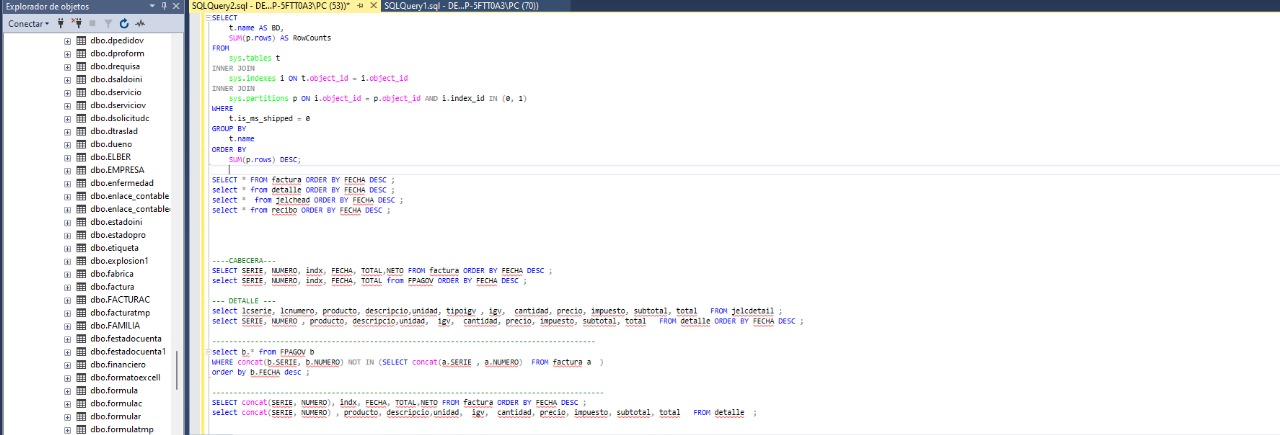
\includegraphics[width=0.9\textwidth]{3/figures/querysql.jpg}
				\caption{Consulta SQL}
				\textit{Fuente: Elaboración propia}
				\label{fig:querysql}
			\end{center}	
		\end{figure}
		
		
		\begin{figure}[H]
			\begin{center}
				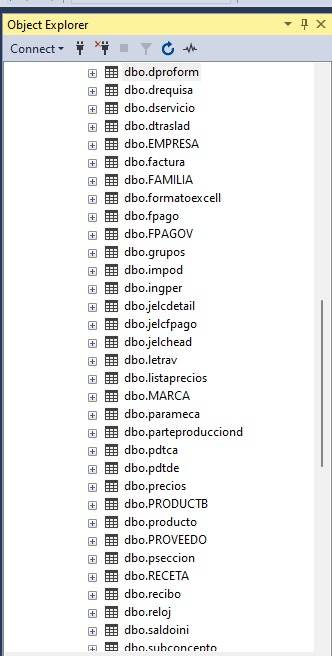
\includegraphics[width=0.5\textwidth]{3/figures/tablaSQL.jpg}
				\caption{Tablas de ventas}
				\textit{Fuente: Elaboración propia}
				\label{fig:tablasql}
			\end{center}	
		\end{figure}
		
		
		
		
		
		%\LaTeX{} is great at typesetting mathematics. Let $X_1, X_2, \ldots, X_n$ be a sequence of independent and identically distributed random variables with
		%\begin{equation}
		%	S_n = \frac{X_1 + X_2 + \cdots + X_n}{n}
		%	= \frac{1}{n}\sum_{i}^{n} X_i
		%	\label{eq1}
		%\end{equation}
		
		%La Ecuación \ref{eq1} denote their mean. Then as $n$ approaches infinity, the random variables $$\sqrt{n}(S_n - \mu)$$ converge in distribution to a normal $\mathcal{N}(0, \sigma^2)$.
		
		
		\section{Técnicas para el procesamiento y análisis de la información}
		Para entrar con más detalles a la metodología se describen los pasos a seguir.
		
		
		\subsection{Metodología de la implementación de la solución}
		El primer paso en el proceso KDD (Knowledge Discovery in Databases) consiste en la comprensión y selección de los datos disponibles, así como en la definición clara de los objetivos de la investigación desde la perspectiva del investigador. Este proceso se fundamenta en el conocimiento previo y adquirido durante el estudio. En el contexto del análisis de tendencias de ventas a lo largo del tiempo, este paso implica examinar minuciosamente aspectos como el monto de la transacción, la fecha y hora de compra, la cantidad adquirida, la categoría de producto (familia) y el producto específico.
		Además, resulta esencial definir con precisión los objetivos específicos de la investigación, tales como la identificación de patrones de comportamiento en las series temporales de ventas. Estos objetivos guían el análisis detallado y permiten enfocar la metodología hacia la detección de patrones útiles que faciliten la toma de decisiones y la optimización de la gestión de demanda en productos perecibles.
		
				
		\begin{figure}[H]
			\begin{center}
				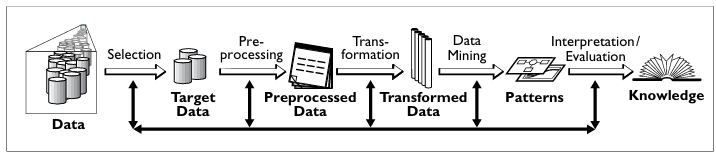
\includegraphics[width=0.9\textwidth]{2/figures/KDD.png}
				\caption{Metodología KDD}
				\textit{Fuente: Fayyad, U., Piatetsky-Shapiro, G.,  Smyth, P. (1996). The KDD process for extracting useful knowledge from volumes of data. Communications of the ACM, 39(11), 27-34.}
				\label{fig:KDD}
			\end{center}	
		\end{figure}
		
		\begin{table}[H]
			\centering
			\caption{Instrumentos de medida para recolección de datos}
			\begin{tabular}{|L{2.7cm}|L{2.5cm}|C{2cm}|C{3.5cm}|C{3.5cm}|}
				\hline 
				Técnica & Instrumento & Origen & Principales ventajas & Principales desventajas\\
				\hline \hline
				Datos de ventas históricas & Registro de ventas(2012-2026) & Registro de la empresa & Obtiene datos cuantitativos sobre las ventas históricas de productos & No proporciona informacion cualitativa sobre los patrones de la demanda  \\
				\hline
				Sistemas de punto de venta (POS) & Hardware POS & Registro en tiempo real de transacciones & Ofrece datos continuos y actualizados sobre las ventas & Dependencia de la confiabilidad del sistema \\
				\hline
				Datos de inventarios & Registro de inventarios & Registro de la empresa & Permite evaluar la relación entre la demanda y la gestión de inventarios Cuantitativamente & No proporciona información sobre factores externos\\
				\hline
%				Análisis de datos climaticos & Datos climáticos & Registros & Permite cuantificar como las condiciones climáticas influyen en la demanda & No considera factores anómalos climáticos\\
%				\hline
				
			\end{tabular}
			\newline
			\newline \textit{Fuente: Elaboración propia}
		\end{table}
		
		Esta comprensión inicial es fundamental para orientar las etapas siguientes de la metodología KDD y garantizar que el análisis de los datos sea relevante y eficaz. La selección de la base de datos adecuada y de las variables para el modelo de aprendizaje automático se realizará utilizando la base de datos proporcionada por la entidad en este caso de estudio.
		
		
		% \subsection{Comprensión del negocio}
		% En la fase inicial, se identificó el problema mediante la comprensión del contexto de la investigación. A partir de esta comprensión, se establecieron los objetivos y requisitos esperados para el proyecto. La siguiente tabla muestra la lista de actividades y tareas planificadas.
		
		% \begin{table}[H]
		% 	\centering
		% 	\caption{Actividades de la comprensión de negocio}
		% 	\begin{tabular}{L{3cm}|L{5cm}|L{5cm}}
				
		% 		Actvidades & Descripción & Tareas \\
		% 		\hline \hline
		% 		Definir problemas, objetivos e hipotesis. & Se definieron los problemas, objetivos, e hipótesis tanto generales como específicos de la investigación. &  
		% 		\begin{itemize}
		% 			\item Identificar la problemática del contexto.
		% 			\item Establecer los objetivos de la investigación.
		% 			\item Formular las hipótesis del estudio.
		% 		\end{itemize}
		% 		\\
		% 		\hline
		% 		Desarrollar la literatura de la investigación. & Se realizó una selección de antecedentes y estudios previos relacionados con la investigación. & 
		% 		\begin{itemize}
		% 			\item Buscar estudios relacionados al tema, la metodología y solución.
		% 		\end{itemize} \\
		% 		\hline	
		% 		Definir metodología de la investigación. & Se definió la metodología a implementarse en el estudio. & 
		% 		\begin{itemize}
		% 			\item Seleccionar la metodología a implementar en base a la investigación de antecedentes.
		% 		\end{itemize}
		% 		\\
		% 		\hline
				
		% 	\end{tabular}
		% 	\newline
		% 	\newline \textit{Fuente: Elaboración propia}
		% \end{table}
		
		
		% \textbf{Actividad 1: } Definir problemas, objetivos e hipótesis.\\
		% Esta actividad describe cómo se identificaron los problemas y se establecieron los objetivos e hipótesis, tanto generales como específicos, de la investigación, basándose en el análisis de la situación problemática actual.\\
		% \textbf{Entregable: } Problemas, objetivos e hipótesis.
		
		% \textbf{Actividad 2: } Desarrollar la literatura de la investigación.\\
		% Una vez definidos los objetivos, se llevó a cabo la búsqueda de fuentes, publicaciones, libros, artículos y material académico relacionado con el contexto, sus características y los métodos empleados para resolver problemas en ese entorno. Además, se desarrolló el marco teórico del estudio.\\
		% \textbf{Entregable: } Antecedentes académicos en la forma de objetivo, base de datos, metodología y resultados en el contexto de la investigación
		
		% \textbf{Actividad 3: } Definir la metodología de la investigación.\\
		% Después de obtener suficientes recursos intelectuales y revisar los trabajos previos necesarios para el desarrollo de la investigación, se analizaron detalladamente cada uno de los antecedentes y se compararon las metodologías implementadas por distintos autores. Al finalizar esta tarea, y con base en la literatura y los procesos más alineados con el presente estudio, se seleccionó la metodología KDD como la opción más adecuada.\\
		% \textbf{Entregable: } Metodología a implementar.
		
		
		\subsection{Comprensión de los datos}
		La investigación incluyó un proceso exhaustivo de exploración, análisis e interpretación de la información recopilada, con el objetivo de identificar patrones, tendencias y relaciones significativas. Este paso es fundamental para garantizar que los datos sean relevantes, precisos y útiles para responder a las preguntas de investigación y alcanzar los objetivos del estudio. El conjunto de datos utilizado abarca 7,340,659 registros de ventas, organizados por familia de productos, correspondientes a los años 2012 al 2026. 
		% Para mayor claridad, se elaboró una tabla que presenta las actividades y tareas realizadas. \ref{tab:compredatos}
		
		% \begin{table}[H]
		% 	\centering
		% 	\caption{Actividades de la Comprensión de los datos}
		% 	\begin{tabular}{L{3cm}|L{5cm}|L{5cm}}
				
		% 		Actvidades & Descripción & Tareas \\
		% 		\hline \hline
		% 		Selección de la base de datos & Base de datos que contenga variables que aporten al modelo y representen significancia al pronóstico & 
		% 		\begin{itemize}
		% 			\item Construir los query en SQL para seleccionar las variables representativas para la ivestigación.
		% 			\item Agrupar las variables por familias para preparar el análisis.
		% 		\end{itemize} \\
		% 		\hline
		% 		Analisis bivariado y univariado & Análisis del comportamiento de las variables y en la descripción y resumen de una sola variable a la vez para entender y representar las características básicas & 
		% 		\begin{itemize}
		% 			\item Construir los scrips en python para analizar variables y pares de variables. 
		% 			\item Entender las características de cada variable.
		% 		\end{itemize} \\
		% 		\hline
		% 		%		Análisis estadístico & Analisis estadístico para interpretar y presentar datos cuantitativos para descubrir patrones, tendencias y relaciones significativas & 
		% 		%		\begin{itemize}
		% 			%			\item Analizar el comportamiento estadístico de cada variable cuantitativa.
		% 			%			
		% 			%		\end{itemize} \\
		% 		%		\hline
		% 	\end{tabular}
		% 	\label{tab:compredatos}
		% 	\newline
		% 	\newline \textit{Fuente: Elaboración propia}
		% \end{table}
		
		
		% \textbf{Actividad 1: }Selección de la base de datos. \\
		% La selección de los datos en SQL implicó escoger una base de datos con variables específicas del negocio dentro de un sistema de gestión de bases de datos (DBMS).
		
		% \begin{figure}[H]
		% 	\begin{center}
		% 		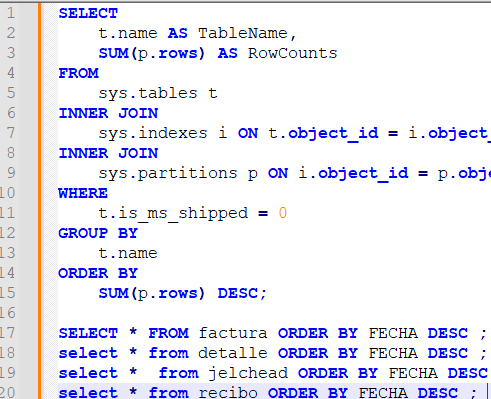
\includegraphics[width=0.6\textwidth]{3/figures/select_tablas.png}
		% 		\caption{Selección de tablas SQL}
		% 		\textit{Fuente: Elaboración propia}
		% 		\label{fig:consultaSQL}
		% 	\end{center}	
		% \end{figure}
		
		\begin{figure}[H]
			\begin{center}
				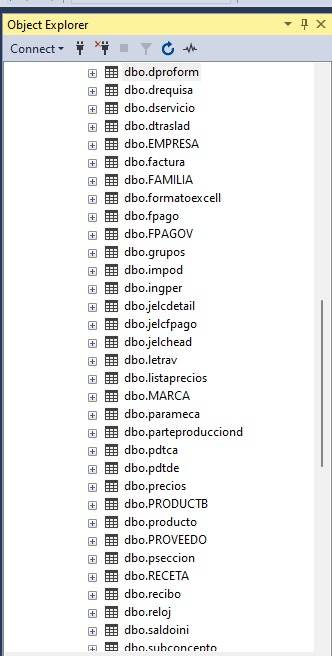
\includegraphics[width=0.6\textwidth]{3/figures/tablaSQL.jpg}
				\caption{Tablas de ventas}
				\textit{Fuente: Elaboración propia}
				\label{fig:tablaSQL}
			\end{center}	
		\end{figure}
		
		
		% \textbf{Entregable: }  Tablas de ventas 
		
		% \textbf{Actividad 2: }Analisis bivariado y univariado. \\
		Se emplearon análisis univariado y bivariado para examinar y comprender los datos. El análisis univariado se centró en describir y resumir una sola variable a la vez, utilizando estadísticas como la media, mediana, moda y varianza, además de visualizaciones como histogramas para revelar la distribución y características específicas de esa variable. Por otro lado, el análisis bivariado se enfocó en explorar la relación entre dos variables, empleando técnicas como tablas de correlación y regresión para identificar patrones, asociaciones y posibles causalidades entre las variables.
	
		\begin{figure}[H]
    \centering
    
    \begin{subfigure}{0.45\textwidth}
        \centering
        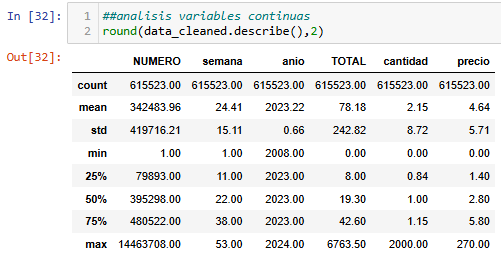
\includegraphics[width=\linewidth]{3/figures/descrip_var.png}
        \caption{Descripción cuantitativa}
        \label{fig:descrip_var}
    \end{subfigure}
    \hfill
    \begin{subfigure}{0.45\textwidth}
        \centering
        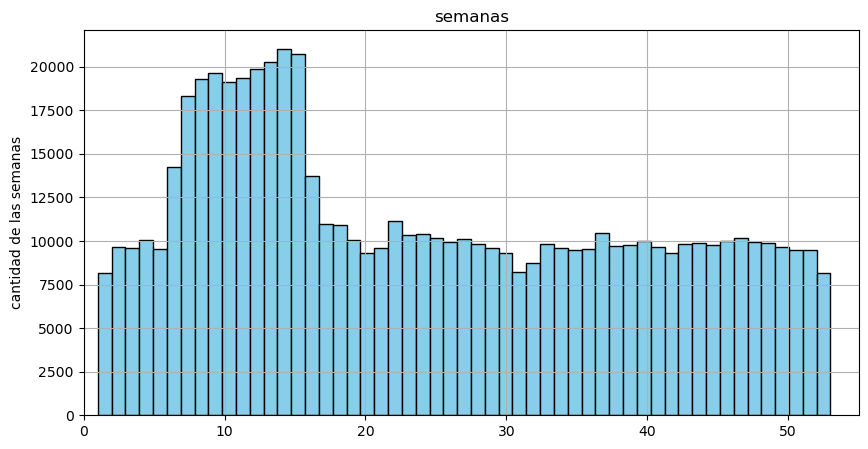
\includegraphics[width=\linewidth]{3/figures/cant_sem.png}
        \caption{Cuantificación de semanas}
        \label{fig:cant_sem}
    \end{subfigure}

    \vspace{0.5cm}

    \begin{subfigure}{0.45\textwidth}
        \centering
        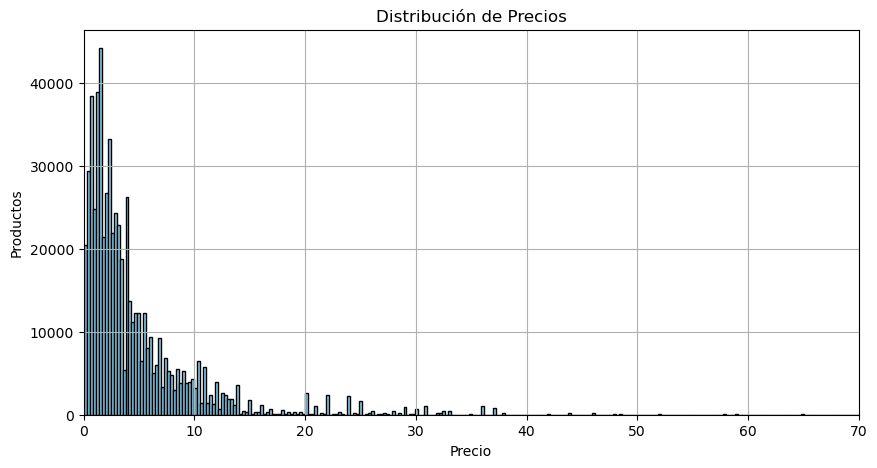
\includegraphics[width=\linewidth]{3/figures/distr_precios.png}
        \caption{Distribución de precio}
        \label{fig:distr_precios}
    \end{subfigure}
    \hfill
    \begin{subfigure}{0.45\textwidth}
        \centering
        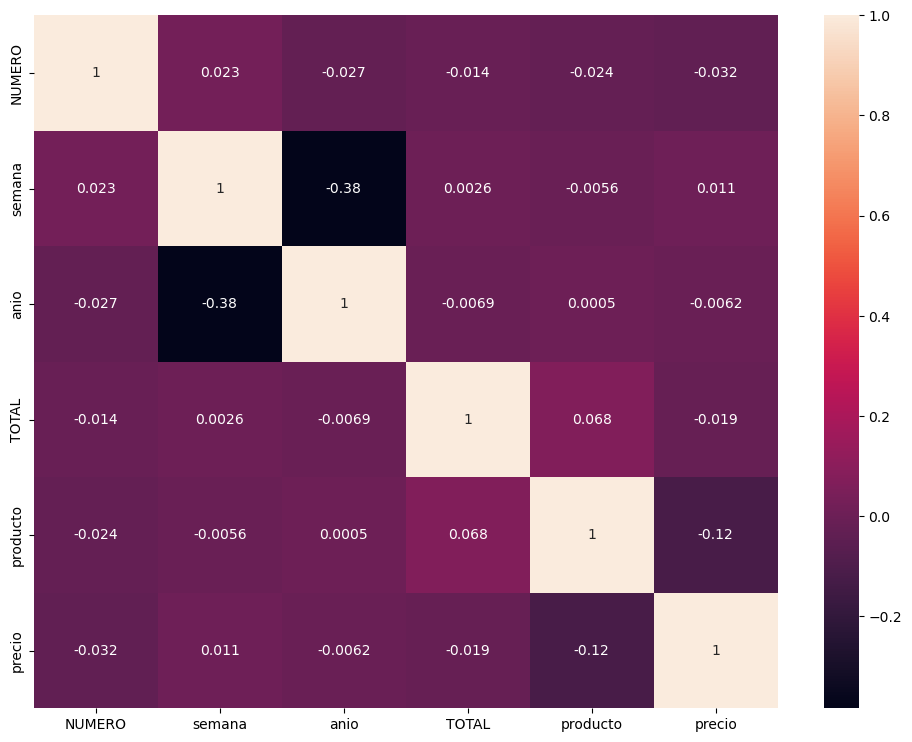
\includegraphics[width=\linewidth]{3/figures/corr_var.png}
        \caption{Correlación de variables}
        \label{fig:corr_var}
    \end{subfigure}

    \caption{Análisis exploratorio de variables}
    \textit{Fuente: Elaboración propia}
    \label{fig:analisis_exploratorio}
\end{figure}
	
		% \begin{figure}[H]
		% 	\begin{center}
		% 		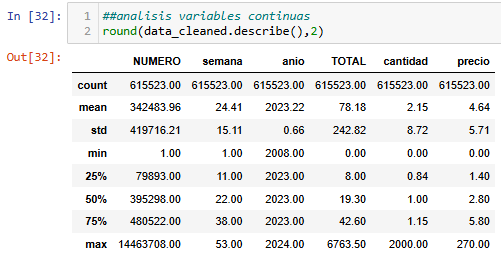
\includegraphics[width=0.6\textwidth]{3/figures/descrip_var.png}
		% 		\caption{Descripción cuantitativa}
		% 		\textit{Fuente: Elaboración propia}
		% 		\label{fig:descrip_var}
		% 	\end{center}	
		% \end{figure}
		
		% \begin{figure}[H]
		% 	\begin{center}
		% 		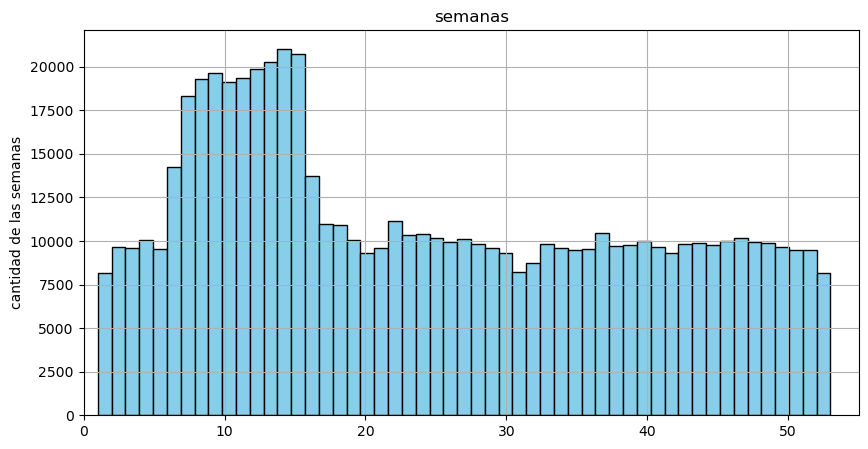
\includegraphics[width=0.6\textwidth]{3/figures/cant_sem.png}
		% 		\caption{Cuantificación de semanas}
		% 		\textit{Fuente: Elaboración propia}
		% 		\label{fig:cant_sem}
		% 	\end{center}	
		% \end{figure}
		
		% \begin{figure}[H]
		% 	\begin{center}
		% 		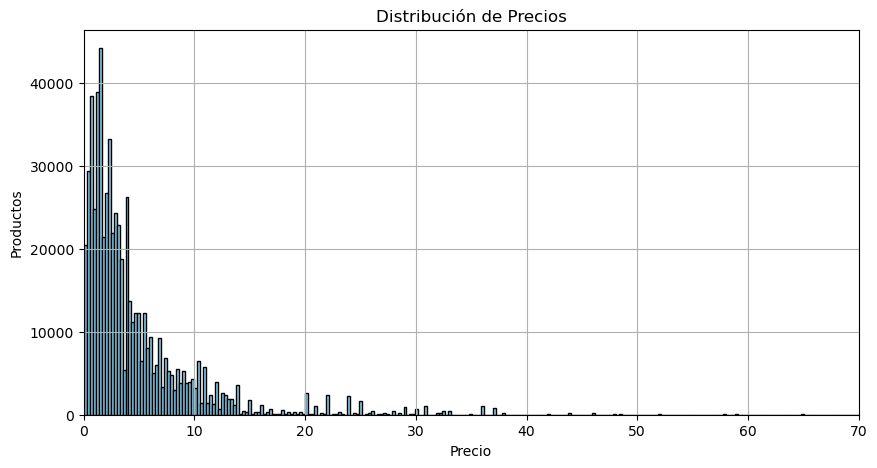
\includegraphics[width=0.6\textwidth]{3/figures/distr_precios.png}
		% 		\caption{Distribución de precio}
		% 		\textit{Fuente: Elaboración propia}
		% 		\label{fig:distr_precios}
		% 	\end{center}	
		% \end{figure}
		
		% \begin{figure}[H]
		% 	\begin{center}
		% 		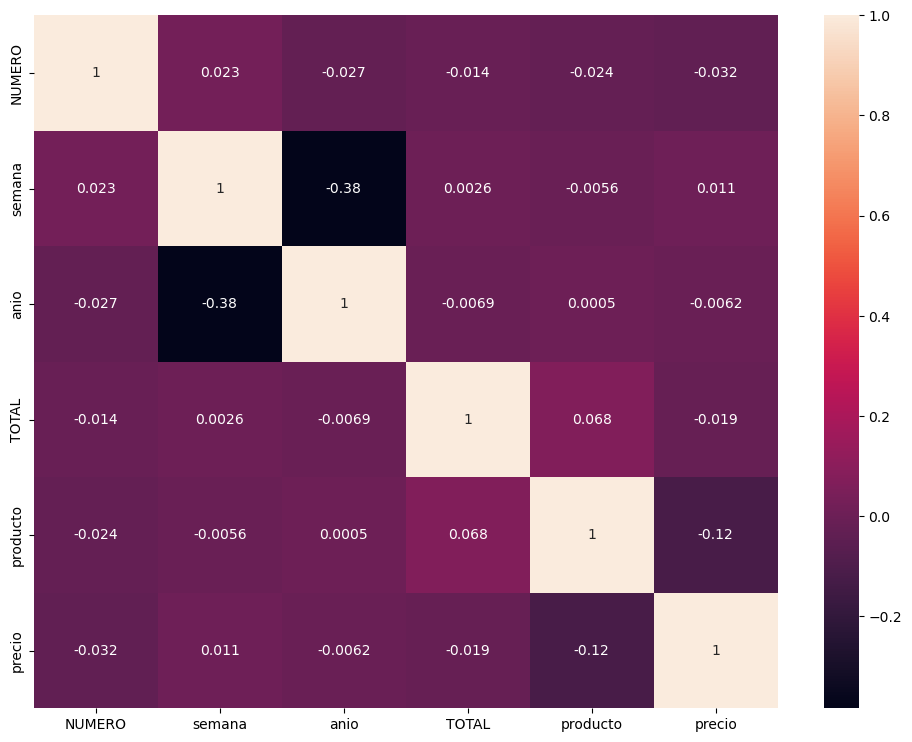
\includegraphics[width=0.6\textwidth]{3/figures/corr_var.png}
		% 		\caption{Correlación de variables}
		% 		\textit{Fuente: Elaboración propia}
		% 		\label{fig:corr_var}
		% 	\end{center}	
		% \end{figure}
		
		El mapa de calor muestra la correlación entre varias variables, como semana, año, total, producto, y precio. En general, las correlaciones son débiles, con solo una correlación negativa moderada entre semana y año (-0.38). Esto sugiere que no hay relaciones lineales fuertes entre las variables, lo cual indica que cada una aporta información única al conjunto de datos. Este análisis preliminar sugiere que no es necesario eliminar ninguna columna por redundancia, ya que las correlaciones no son suficientemente altas.
		
		% \textbf{Entregable: } Análisis estadístico de variables
		
		\subsection{Pre-Procesamiento}
		% Una vez integrada la información en la base de datos, se desarrolló la etapa de preprocesamiento de datos, cuyo objetivo principal fue garantizar la calidad, consistencia y confiabilidad de la información antes de realizar el análisis exploratorio y el entrenamiento de los modelos predictivos.

En esta fase se efectuó, en primer lugar, la normalización de los nombres de las variables, con la finalidad de mantener una estructura homogénea dentro del conjunto de datos y evitar inconsistencias durante el procesamiento. Posteriormente, las variables de tipo temporal fueron convertidas a un formato de fecha estándar, permitiendo ordenar cronológicamente los registros y facilitar el análisis de series temporales.

Asimismo, las variables numéricas relacionadas con las ventas fueron transformadas al tipo de dato correspondiente para asegurar su correcta interpretación por parte de los algoritmos de análisis. Durante este proceso también se identificaron y eliminaron registros incompletos, inconsistentes o con valores inválidos, especialmente aquellos asociados a fechas o montos de venta no reconocidos.

Después de la limpieza inicial, los datos fueron ordenados secuencialmente según la variable temporal. Este procedimiento resulta fundamental en problemas de predicción temporal, debido a que los modelos requieren preservar la relación cronológica entre observaciones históricas y futuras.

Posteriormente, se realizó la segmentación de la información según criterios específicos de análisis, tales como la sede y la familia de productos. Esta segmentación permitió trabajar con subconjuntos de datos más homogéneos y representativos, contribuyendo a mejorar la precisión y pertinencia de los modelos predictivos.

Finalmente, el preprocesamiento permitió obtener un conjunto de datos estructurado, consistente y preparado para las etapas posteriores de análisis exploratorio, entrenamiento y evaluación de modelos de predicción.
		
		
		% \subsection{Procesamiento}
		% El segundo paso en la metodología KDD se centra en la preparación de los datos de transacciones de ventas de manera diaria. Este proceso implica realizar operaciones básicas de limpieza y depuración, eliminando ruido y valores atípicos que puedan afectar la calidad y precisión de los resultados. Además, se recopila información relevante para entender y modelar el ruido presente en los datos, lo que facilita una interpretación más clara de los patrones y tendencias. Se implementan también estrategias para gestionar campos de datos que carecen de información cronológica, asegurando así la coherencia y cohesión de los datos para un análisis efectivo.
		
		% \subsection{Transformación}
		% En el tercer paso de la metodología KDD, se realiza la transformación de datos para adecuarlos al análisis, centrándose en agrupar los productos por familias. Esta fase implica identificar características que representen eficazmente los datos y que se ajusten a los objetivos específicos de la tarea de análisis. Según estos objetivos, se seleccionan las características más relevantes para proporcionar información significativa sobre las ventas. Además, se aplican técnicas para reducir la complejidad de los datos o encontrar representaciones más concisas y manejables. Este proceso es fundamental para simplificar la estructura de los datos y facilitar un análisis más eficiente y efectivo.
		
		%\subsection{Modelado}
		%En el cuarto paso de la metodología KDD, se profundiza en la minería de datos para predecir las ventas. Aquí, la selección adecuada de algoritmos es crucial para descubrir patrones significativos en los datos, considerando su naturaleza, los objetivos de la predicción y la complejidad del análisis requerido. Se ajustan los parámetros de los algoritmos para mejorar el rendimiento del modelo predictivo y se evalúa la idoneidad de cada método para asegurar predicciones precisas sobre las ventas.
		%
		%\subsection{Evaluación}
		%En el cuarto paso de la metodología KDD, se aborda la interpretación de patrones y la selección de algoritmos para predecir las ventas semanales, segmentadas por familias como verduras, frutas, carnes, entre otros. Es crucial evaluar la efectividad de los algoritmos en la detección de patrones significativos en los datos y estar preparado para ajustar el análisis retrocediendo a pasos anteriores si es necesario.
		%La capacidad de visualizar los patrones extraídos es esencial para comprender la serie temporal de las ventas, lo que facilita la identificación de las familias con mayor porcentaje de venta y la estimación de presupuestos semanales basados en la demanda. Durante este proceso, se eliminan patrones redundantes o irrelevantes para centrarse en aquellos más pertinentes para el análisis de ventas. Finalmente, estos patrones se convierten en términos comprensibles para los usuarios, facilitando la toma de decisiones informadas y la implementación de estrategias efectivas de compra de mercadería.
		
		\subsection{Modelamiento}
		Al concluir la etapa del preprocesamiento, las variables pudieron ser utilizadas para los modelos de cada modalidad, que fueron diseñados siguiendo las actividades de la Tabla \ref{tab:act_model}
		
		\begin{table}[H]
			\centering
			\caption{Actividades de fase modelamiento}
			\begin{tabular}{L{3cm}|L{5cm}|L{5cm}}
				
				Actvidades & Descripción & Tareas \\
				\hline \hline
				Desarrollar modelos predictivos para data estructurada. & Implementación de un mínimo de 8 modelos de forecasting para entrenarlos y seleccionar el mejor para la data.  &  Escoger los modelos para entrenarlos y ver cual es el mejor modelo para realizar los pronósticos de ventas.
				
				\\
				\hline
				Seleccionar las métricas para la evaluación del modelo. & Implementación las métricas para poder evaluar a los modelos implementados. & Escoger las métricas que definirán cual modelo será mejor para realizar los pronósticos de venta (R2, MSE, RMSE y MAPE).
				\\
				\hline	
				
			\end{tabular}
			\newline
			\newline \textit{Fuente: Elaboración propia}
			\label{tab:act_model}
		\end{table}
		
		\textbf{Actividad 1: } Desarrollar modelos predictivos para data estructurada.\\
		En esta actividad, se diseñó la arquitectura que se utilizó para los datos estructurados. Para ello, se llevó a cabo un benchmarking sobre los modelos a utilizar:
		\begin{itemize}
			\item \textbf{ARIMA: } ARIMA es un modelo estadístico utilizado para analizar y predecir series temporales. Combina la parte autoregresiva (AR), que utiliza las observaciones pasadas para predecir valores futuros, con la parte de media móvil integrada (IMA), que maneja la variabilidad y tendencia de los datos.
			\item \textbf{LSTM: } LSTM es un tipo de red neuronal recurrente (RNN) diseñada para modelar secuencias temporales y dependencias a largo plazo. Es capaz de aprender dependencias temporales en los datos y es especialmente efectiva en problemas donde las relaciones entre eventos en el tiempo son importantes.
			\item \textbf{LINEAR REGRESSION: } La regresión lineal es un modelo estadístico que examina la relación lineal entre una variable dependiente y una o más variables independientes. El objetivo es encontrar la línea (o plano en casos de múltiples variables) que mejor se ajuste a los datos, minimizando la suma de los errores cuadráticos.
			\item \textbf{XGBOOST: } XGBoost es una implementación optimizada del algoritmo de gradient boosting, que se utiliza ampliamente en problemas de aprendizaje supervisado, tanto para clasificación como para regresión. Utiliza árboles de decisión como modelos base y se enfoca en mejorar el rendimiento a través de técnicas como la regularización y el manejo eficiente de conjuntos de datos grandes.
			\item \textbf{SVR: } SVR es una variante de las máquinas de vectores de soporte (SVM) adaptada para problemas de regresión. A diferencia de los métodos de regresión lineal, SVR utiliza vectores de soporte en un espacio de alta dimensión para predecir valores continuos, buscando la función que mejor se ajuste a los datos mientras mantiene un margen de error aceptable.
			\item \textbf{RANDOM FOREST: } Random Forest es un conjunto de árboles de decisión, donde cada árbol es construido de manera independiente y con muestras de datos aleatorias. La predicción final se obtiene por votación o promediando las predicciones individuales de los árboles, lo que mejora la precisión y reduce el sobreajuste.
			\item \textbf{DECISION TREE: } Un árbol de decisión es una estructura de modelo de aprendizaje automático que divide un conjunto de datos en subconjuntos más pequeños basados en características específicas de las variables predictoras. Cada nodo representa una característica y cada hoja representa un resultado o decisión.
			\item \textbf{PROPHET: } Prophet es un modelo desarrollado por Facebook para realizar pronósticos de series temporales. Es especialmente útil cuando se cuenta con datos estacionales, festivos o fluctuaciones regulares, y permite manejar datos con puntos faltantes o valores atípicos. Es fácil de usar y flexible para ajustar tendencias y patrones estacionales.
			\item \textbf{GRADIENT BOOSTING: } Gradient Boosting es un algoritmo de aprendizaje supervisado que construye modelos de forma secuencial, donde cada nuevo modelo corrige los errores del anterior. Utiliza árboles de decisión como modelos base y optimiza una función de pérdida mediante el descenso de gradiente, logrando alta precisión en tareas de regresión y clasificación.

\item \textbf{KNN (K-Nearest Neighbors): } KNN es un algoritmo de aprendizaje basado en instancias que realiza predicciones basándose en los datos más cercanos en el espacio de características. Para regresión, el valor predicho se obtiene como el promedio de los valores de sus vecinos más cercanos, lo que lo hace simple pero efectivo en ciertos contextos.

\item \textbf{HOLT-WINTERS: } Holt-Winters es un método de suavizamiento exponencial utilizado para series temporales que presentan tendencia y estacionalidad. Este modelo combina componentes de nivel, tendencia y estacionalidad para realizar predicciones más precisas en datos con patrones periódicos.

\item \textbf{NAIVE: } El modelo Naive es un enfoque simple de pronóstico en series temporales que asume que el valor futuro será igual al último valor observado. A pesar de su simplicidad, se utiliza como modelo base para comparar el rendimiento de modelos más complejos.

\item \textbf{SARIMA: } SARIMA (Seasonal ARIMA) es una extensión del modelo ARIMA que incorpora componentes estacionales. Permite modelar tanto patrones no estacionales como estacionales en series temporales, siendo útil cuando los datos presentan ciclos repetitivos a lo largo del tiempo.
		\end{itemize}
		
		Con base en la revisión de estudios previos, se observó que los modelos LSTM, Regresión Lineal y Árbol de Decisión ofrecieron los mejores resultados en experimentos similares. Dado que el objetivo de la investigación era implementar un modelo de regresión, se decidió utilizar Regresion Lineal para el análisis de los datos estructurados.
		
		\textbf{Diseño de la Arquitectura Regresion Lineal Multiple}
		
		La ecuación general de la regresión lineal múltiple se define como:  
		
		\begin{equation}
		Y = \beta_0 + \beta_1 X_1 + \beta_2 X_2 + \cdots + \beta_n X_n + \epsilon
		\end{equation}
		
		Donde:  
		\begin{itemize}
			\item \( Y \): Variable dependiente o respuesta.
			\item \( X_1, X_2, \dots, X_n \): Variables independientes o explicativas.
			\item \( \beta_0 \): Intercepto o término constante.
			\item \( \beta_1, \beta_2, \dots, \beta_n \): Coeficientes de las variables independientes, que representan su contribución al valor de \( Y \).
			\item \( \epsilon \): Error residual, que captura las desviaciones no explicadas por el modelo.
		\end{itemize}
		
		El objetivo es estimar los coeficientes \( \beta_0, \beta_1, \dots, \beta_n \) que minimicen la suma de los errores al cuadrado (Método de Mínimos Cuadrados Ordinarios):  
		
		\begin{equation}
		\text{Minimizar: } \sum_{i=1}^m \left( Y_i - \hat{Y}_i \right)^2
		\end{equation}
		
		Donde \( \hat{Y}_i \) es el valor predicho para la \( i \)-ésima observación.  
		
%		Para diseñar la arquitectura del modelo LSTM, se evaluaron diversas metodologías y estrategias. Finalmente, se seleccionaron las siguientes 12 pautas fundamentales para su implementación:
%		
%		\begin{enumerate}
%			\item Comenzar con al menos 2 capas LSTM para capturar dependencias a largo plazo en los datos secuenciales. 
%			\item El número de unidades en las capas LSTM puede variar dependiendo de la complejidad del problema y la cantidad de datos disponibles. Puedes experimentar con diferentes números de unidades, como 50, 100 o más.
%			\item Utilizar una capa densa con una unidad para la predicción de ventas, con función de activación lineal.
%			\item Utilizar la función de activación 'tanh' o 'sigmoid' para las capas LSTM para introducir no linealidades en el modelo.
%			\item Aplicar dropout después de cada capa LSTM para mejorar la generalización del modelo, con una tasa recomendada del 0.2 o ajustada según experimentación.
%			\item Escalar los datos secuenciales utilizando métodos como MinMaxScaler o StandardScaler según la naturaleza de los datos y su distribución.
%			\item Utilizar métricas como el error cuadrático medio (MSE) o el error absoluto medio (MAE) para evaluar el rendimiento del modelo de predicción.
%			\item Comenzar con un número adecuado de épocas, por ejemplo, 20 épocas, y ajustar según la mejora en la precisión y la reducción de la pérdida. Aumentar gradualmente hasta 100 épocas si es necesario para mejorar el rendimiento del modelo LSTM.
%			\item Utilizar la función 'train\_test\_split' para dividir los datos en conjuntos de entrenamiento y prueba. Asegúrate de que los datos estén divididos de manera que se mantenga la secuencia temporal, es decir, no barajar los datos.
%			\item No aplica directamente para predicción de ventas, pero asegúrate de que tus datos están correctamente representados y no tienen sesgos significativos que puedan afectar la predicción.
%			\item Utilizar el optimizador 'Adam' con sus configuraciones por defecto para el aprendizaje de los pesos de la red neuronal LSTM.
%			\item Aplicar técnicas de regularización como L2 para evitar el sobreajuste del modelo 
%			
%		\end{enumerate}
		
		\textbf{Entregable: } Modelo Regresion Lineal para el pronostico de ventas.
		
		\textbf{Actividad 2: } Seleccionar las métricas para la evaluación del modelo
		En esta actividad, se llevó a cabo una investigación basada en el estado del arte para identificar las métricas ma´s utilizadas en investigaciones previas. Se encontró que las métricas más frecuentemente empleadas fueron las siguientes:
		
		
		\begin{itemize}
			\item \textbf{RMSE: } Calcula la raíz cuadrada de la media de los cuadrados de los errores entre las predicciones de un modelo y los valores reales. Es útil para medir el nivel de error promedio de las predicciones en la misma unidad que los datos originales.
			\item \textbf{MSE: } Calcula el promedio de los cuadrados de los errores entre las predicciones de un modelo y los valores reales. Proporciona una medida de la varianza de los errores, penalizando más fuertemente los errores grandes.
			\item \textbf{MAPE: } Calcula el promedio del porcentaje absoluto de los errores entre las predicciones de un modelo y los valores reales. Es útil para evaluar la precisión relativa de un modelo, especialmente en situaciones donde se desea conocer el error porcentual promedio. 
		\item \textbf{R2: } Calcula el coeficiente de determinación, que mide la proporción de la variabilidad en los datos que es explicada por el modelo. Un valor de R2 cercano a 1 indica un buen ajuste del modelo a los datos, mientras que un valor cercano a 0 indica un ajuste pobre.
		\end{itemize}
		
		De acuerdo a la anterior lista, estas métricas ayudarán a:
		
		\begin{itemize}
			\item Evaluar la precisión y el rendimiento de modelos predictivos en comparación con los valores reales.
			\item Cuantificar el nivel de error y la discrepancia entre las predicciones del modelo y los datos observados.
			\item Optimizar y ajustar los parámetros del modelo para minimizar el error y mejorar la precisión de las predicciones.
		\end{itemize}
		
% 		Estas métricas proporcionan una base sólida para la evaluación rigurosa de modelos predictivos en diversas aplicaciones, facilitando la toma de decisiones informadas y la mejora continua del rendimiento del modelo.\\
		
% 		Las métricas señaladas se calculan de la siguiente manera: \\
		
% 		\textbf{RMSE (Root Mean Square Error)}\\
		
% 		\textbf{Calcular los errores individuales: } Para cada predicción \(\hat{y}_i\) y su valor real \(y_i\), calcula el error cuadrático.
		
% 		\begin{equation} 
% 			\text{Error}_i = (\hat{y}_i - y_i)^2
% 		\end{equation}
		
% 		\textbf{Calcular el promedio de los errores cuadráticos: } Luego, calcula el promedio de estos errores cuadráticos sobre todos los puntos de datos.
		
% 		\begin{equation} 
% 			\text{MSE} = \frac{1}{n} \sum_{i=1}^{n} (\hat{y}_i - y_i)^2
% 		\end{equation}
		
% 		\textbf{Calcular la raíz cuadrada del MSE: } Finalmente, obtén el RMSE tomando la raíz cuadrada del MSE.
% 		\begin{equation}
% 			\text{RMSE} = \sqrt{\text{MSE}}
% 		\end{equation}
		
% 		\textbf{MSE (Mean Squared Error)}\\
% 		\textbf{Calcular los errores individuales: } Para cada predicción \(\hat{y}_i\) y su valor real \(y_i\), calcula el error cuadrático como en el paso 1 del RMSE:
% 		\begin{equation}
% 			\text{Error}_i = (\hat{y}_i - y_i)^2
% 		\end{equation}
		
% 		\textbf{Calcular el promedio de los errores cuadráticos: } Luego, calcula el promedio de estos errores cuadráticos sobre todos los puntos de datos. 
		
% 		\begin{equation}
% 			\text{MSE} = \frac{1}{n} \sum_{i=1}^{n} (\hat{y}_i - y_i)^2
% 		\end{equation}
		
% 		\textbf{MAPE (Mean Absolute Percentage Error)}\\
% 		\textbf{Calcular los errores porcentuales individuales: } Para cada predicción \(\hat{y}_i\) y su valor real \(y_i\), calcula el error porcentual absoluto.
		
% 		\begin{equation}
% 			Error_i = \left( \frac{y_i - \hat{y}_i}{y_i} \right) \times 100
% 		\end{equation}
		
% 		\textbf{Calcular el promedio de los errores porcentuales: } Luego, calcula el promedio de estos errores porcentuales sobre todos los puntos de datos.
% 		%%%%%AGREGAR R2
% 		\begin{equation}
% 			\text{MAPE} = \frac{1}{n} \sum_{i=1}^n \left( \frac{|y_i - \hat{y}_i|}{y_i} \right) \times 100
% 		\end{equation}
		
% 		\textbf{Entregable: } Modelo LSTM entrenado con sus respectivas métricas.
		
% 		%%%%%%%%%%%%%%%%%%%
% 		\textbf{MAE (Mean Absolute Error): } El MAE es una métrica utilizada para evaluar la precisión de modelos de regresión. Mide el promedio de los errores absolutos entre los valores reales y los valores predichos, sin considerar la dirección del error. Es fácil de interpretar, ya que expresa el error promedio en las mismas unidades que la variable objetivo.
% 		\textbf{Fórmula del MAE: }
% 		\[
% 		MAE = \frac{1}{n} \sum_{i=1}^{n} \left| y_i - \hat{y}_i \right|
% \]
% \textbf{R2 (Coeficiente de Determinación): } El R2 es una métrica que mide la proporción de la variabilidad en los datos que es explicada por el modelo de regresión. Un valor de R2 cercano a 1 indica que el modelo explica la mayor parte de la variabilidad, mientras que un valor cercano a 0 indica que el modelo no explica bien los datos.
% \textbf{Fórmula del R2: }
% \[
% R^2 = 1 - \frac{\sum_{i=1}^{n} (y_i - \hat{y}_i)^2}{\sum_{i=1}^{n} (y_i - \bar{y})^2}
% \]
% Donde \( \bar{y} \) es la media de los valores reales \( y_i \).

		\subsection{Evaluación}
		Esta fase comprende la evaluación de los modelos desarrollados en la investigación a través de las métricas de regresión seleccionadas y explicadas en la sección 3.3.6. En la Tabla \ref{tab:act_eva} se indican las actividades y tareas seguidas para esta etapa.
		
		\begin{table}[H]
			\centering
			\caption{Actividades de fase evaluación}
			\begin{tabular}{L{3cm}|L{5cm}|L{5cm}}
				
				Actvidades & Descripción & Tareas \\
				\hline \hline
				Evaluar el modelo predictivo & Evaluación del desempeño del modelo LSTM   & Ejecutar experimentos para definir hiperparámetros.		
				\\
				\hline
				Interpretar las métricas obtenidas & Observar los resultados de las métricas obtenidas permite inferir si el modelo puede ser un predictor confiable para los pronósticos. & Interpretar los resultados obtenidos de las métricas permite extraer conclusiones fundamentales sobre el rendimiento del modelo.
				\\
				\hline		
			\end{tabular}
			\newline
			\newline \textit{Fuente: Elaboración propia}
			\label{tab:act_eva}
		\end{table}
		
		\textbf{Actividad 1:} Evaluar el modelo predictivo.\\
		En esta actividad, se procedió inicialmente con el entrenamiento de todos los modelos utilizando datos recopilados durante aproximadamente 3 años, que incluyen las ventas semanales de la familia con la que se cuenta con mayor cantidad de datos históricos. Este proceso de entrenamiento fue fundamental para ajustar los modelos y capturar patrones y tendencias significativas basadas en un conjunto de datos robusto y representativo.
		Para optimizar el rendimiento de los modelos, se llevaron a cabo entre 3 y 5 experimentos por cada diseño de modelo, explorando diversas combinaciones y ajustes de hiperparámetros en cada iteración. Esta estrategia sistemática permitió evaluar cómo diferentes configuraciones afectan el rendimiento del modelo en términos de métricas críticas como precisión, error y capacidad de generalización.
		Los experimentos no solo se centraron en la optimización de hiperparámetros, sino también en la selección de técnicas de preprocesamiento de datos y ajustes de arquitectura del modelo. Cada iteración fue diseñada para obtener insights valiosos sobre qué configuraciones maximizan la capacidad del modelo para realizar pronósticos precisos y confiables de las ventas semanales.
		Este enfoque riguroso y metódico no solo aseguró la mejora continua del rendimiento predictivo, sino que también proporcionó una base sólida para la toma de decisiones informadas sobre la implementación y refinamiento del modelo finalmente seleccionado.\\
		
		\textbf{Entregable: } Modelo Regresión Lineal Entrenado y Ajustado.
		
		\textbf{Actividad 2: } Interpretar las métricas obtenidas.\\
		En esta actividad, se procedió inicialmente a realizar un análisis exhaustivo de las métricas obtenidas del modelo Regresion Lineal entrenado y ajustado. Estas métricas fueron meticulosamente calculadas para evaluar el desempeño del modelo en la predicción precisa de las ventas semanales, utilizando datos históricos recopilados durante aproximadamente 5 años.\\
		Durante el análisis, se focalizó en métricas fundamentales como el RMSE (Root Mean Square Error), MSE (Mean Squared Error) y MAPE (Mean Absolute Percentage Error). Estas métricas proporcionaron una evaluación cuantitativa del nivel de precisión y error del modelo en comparación con las ventas reales observadas en el período de entrenamiento.\\
		El estudio detallado de estas métricas permitió extraer conclusiones significativas sobre la capacidad del modelo para capturar variaciones y patrones en las ventas semanales. Además, facilitó la identificación de posibles áreas de mejora en términos de ajustes adicionales de hiperparámetros o refinamientos en la arquitectura del modelo Regresión Lineal.
		Este análisis crítico y sistemático es esencial para tomar decisiones informadas sobre la implementación y el desarrollo continuo del modelo Regresión Lineal en aplicaciones futuras de pronóstico de ventas. Asimismo, asegura un mejor rendimiento predictivo y una mayor precisión en la proyección de tendencias comerciales, beneficiando así la toma de decisiones estratégicas en el contexto empresarial.\\
		
		\textbf{Entregable: } Resultados de las métricas  MSE, RMSE, MAPE.
		
		\subsection{Despliegue}
		En la última fase de la metodología seguida, se implementó el modelo propuesto después de completar su entrenamiento y evaluación correspondiente. Esta etapa final fue crucial para poner a prueba la capacidad predictiva del modelo en un entorno operativo real. Las actividades detalladas realizadas durante esta fase se describen en la Tabla \ref{tab:fase_despl}, proporcionando una visión completa de los pasos ejecutados para asegurar la integración efectiva del modelo en la aplicación práctica.
		
		\begin{table}[H]
			\centering
			\caption{Actividades de fase Despliegue}
			\begin{tabular}{L{3cm}|L{5cm}|L{5cm}}
				
				Actvidades & Descripción & Tareas \\
				\hline \hline
				Diseñar prototipo de sistemas con modelo propuesto. & Diseño del prototipo del sistema que integrará la captura de datos con el modelo propuesto para predecir las ventas. &  
				\begin{itemize}
					\item Diseñar una estructura de prototipo de sistema conformado por captura de datos y modelo propuesto.
					\item Cargar complementos del modelo.
				\end{itemize}
				\\
				\hline
				Ejecutar el prototipo y integrarlo con el modelo desarrollado. & Ejecución del sistema prototipo en tiempo real con proyectos de tecnología de campañas vigentes. &
				\begin{itemize}
					\item Ejecutar prototipo con dirección web de proyecto consultado.
					\item Clasificar el estado de financiamiento a partir del resultado predicho.
				\end{itemize}
				\\
				\hline		
			\end{tabular}	
			\newline
			\newline \textit{Fuente: Elaboración propia}
			\label{tab:fase_despl}
		\end{table}
		
		Después de analizar el rendimiento de cada modelo, tanto individualmente como el modelo final, se compararon los resultados con los antecedentes disponibles. Luego, se llevó a cabo una prueba piloto donde se ejecutó el modelo ensamblado entrenado, se obtuvieron sus características y se realizaron predicciones tanto del presupuesto para cada familia de productos como de la cantidad de productos necesarios para realizar un pedido.
		
		\textbf{Actividad 1: } Diseñar prototipo de sistema con modelo propuesto\\
		En esta actividad, se diseñó el prototipo del sistema que integra el modelo propuesto para optimizar la gestión de inventarios y mejorar la precisión en las proyecciones de demanda. El sistema fue concebido para utilizar datos históricos y variables clave, permitiendo una planificación más eficiente de las operaciones y una mejor adaptación a las fluctuaciones del mercado.\\
		\textbf{Entregable: }Arquitectura del prototipo del sistema integrado.
		
		\textbf{Actividad 2: } Ejecutar prototipo con proyectos tecnológicos vigentes.
		En esta actividad, se ejecuta el prototipo web diseñado para implementar el modelo, facilitando la visualización y la posibilidad de realizar un pedido automático de productos. Este sistema web fue desarrollado con el fin de integrar de manera eficiente el modelo predictivo, permitiendo a los usuarios interactuar de forma intuitiva con las predicciones de demanda y facilitando la automatización del proceso de pedidos en tiempo real.\\
		\textbf{Entregable: } Plataforma web con los resultados de los pronósticos obtenidos.
		
		
		%%%%%%%%%%%%%%%%%%%%%%%%%
		
		
		
		%%%%%%%%%%%%%%%%%%%%%%%%%%%%%%%%%%%%%%%%%%%%%%%%%
		
		
		%You can make lists with automatic numbering \dots
		%\begin{enumerate}
		%	\item Like this,
		%	\item and like this.
		%\end{enumerate}
		%\dots or bullet points \dots
		%\begin{itemize}
		%	\item Like this,
		%	\item and like this.
		%\end{itemize}
		
		\section{Metodología para la medición de resultados de la implementación}
		Las métricas empleadas para evaluar la precisión de los modelos fueron el Error Absoluto Medio (MAE), el Error Cuadrático Medio (MSE), la Raíz del Error Cuadrático Medio (RMSE), el Error Porcentual Absoluto Medio (MAPE) y el coeficiente de determinación R$^2$. Estas métricas permitieron comparar las predicciones generadas por los modelos con los valores reales de demanda observados en el conjunto de prueba.

\subsection{Error Absoluto Medio}

El Error Absoluto Medio mide la magnitud promedio del error entre los valores reales y los valores pronosticados. Esta métrica permite interpretar el error en las mismas unidades de la variable objetivo, por lo que resulta útil para evaluar cuánto se desvía, en promedio, la predicción respecto a la demanda real.

\begin{equation}
MAE = \frac{1}{n}\sum_{i=1}^{n}|y_i-\hat{y}_i|
\end{equation}

\subsection{Error Cuadrático Medio}

El Error Cuadrático Medio calcula el promedio de los errores elevados al cuadrado. Esta métrica penaliza con mayor intensidad los errores grandes, por lo que permite identificar modelos que presentan desviaciones significativas respecto a los valores reales.

\begin{equation}
MSE = \frac{1}{n}\sum_{i=1}^{n}(y_i-\hat{y}_i)^2
\end{equation}

\subsection{Raíz del Error Cuadrático Medio}

La Raíz del Error Cuadrático Medio representa la raíz cuadrada del MSE. Su principal ventaja es que expresa el error en la misma unidad de la variable analizada, facilitando la interpretación del desempeño del modelo.

\begin{equation}
RMSE = \sqrt{\frac{1}{n}\sum_{i=1}^{n}(y_i-\hat{y}_i)^2}
\end{equation}

\subsection{Error Porcentual Absoluto Medio}

El Error Porcentual Absoluto Medio mide el error promedio en términos porcentuales. Esta métrica permite conocer qué tan alejada se encuentra la predicción respecto al valor real en términos relativos, lo cual facilita la comparación del desempeño entre modelos.

\begin{equation}
MAPE = \frac{1}{n}\sum_{i=1}^{n}\left|\frac{y_i-\hat{y}_i}{y_i}\right|\times 100
\end{equation}

\subsection{Coeficiente de determinación}

El coeficiente de determinación permite medir la proporción de variabilidad de la demanda real que es explicada por el modelo. Un valor de R$^2$ más cercano a 1 indica una mayor capacidad explicativa del modelo sobre el comportamiento de la demanda.

\begin{equation}
R^2 = 1-\frac{\sum_{i=1}^{n}(y_i-\hat{y}_i)^2}{\sum_{i=1}^{n}(y_i-\bar{y})^2}
\end{equation}
		
		
		% \subsection{Raíz del error cuadrático medio (RMSE)}
		% El término utilizado para denotar el error que surge de la diferencia entre los valores predichos y los valores observados por un modelo o estimador es conocido como error cuadrático medio (RMSE). Esta medida se obtiene al calcular la raíz cuadrada de la media de los errores cuadráticos, lo cual refleja la disparidad entre los valores reales y los valores pronosticados. Es importante destacar que el RMSE, al ser siempre positivo, donde valores menores indican un ajuste más acertado de los datos al modelo. La formulación de este concepto se detalla en la siguiente sección.
		
		% \begin{equation}  
		% 	\label{eq:RMSE}
		% 	\hat{y}_i = \sqrt{\frac{\sum_{i=1}^{n} (y_i - \hat{y}_i)^2}{n}}
		% \end{equation}
		
		% \subsection{Error cuadrático medio (MSE)}
		% El término utilizado para medir la discrepancia entre los valores observados y los valores predichos por un modelo o estimador es conocido como el \textit{Error Cuadrático Medio} (\textit{Mean Squared Error}, MSE). Esta métrica se calcula como el promedio de los cuadrados de las diferencias entre los valores reales y los valores estimados. El MSE proporciona una medida global del error del modelo, donde valores más bajos indican un mejor ajuste de los datos al modelo. Es importante destacar que el MSE siempre es no negativo, ya que los errores al cuadrado eliminan cualquier signo.
		
		% La formulación matemática del MSE se presenta a continuación:
		
		% \begin{equation}
		% \text{MSE} = \frac{1}{n} \sum_{i=1}^{n} (y_i - \hat{y}_i)^2
		% \end{equation}
		
		% \subsection{Error Porcentual Absoluto Medio (MAPE)}
		% El \textit{Error Porcentual Absoluto Medio} (\textit{Mean Absolute Percentage Error}, MAPE) es una métrica utilizada para medir la precisión de un modelo de predicción. Representa el promedio de los errores absolutos expresados en porcentaje, lo que permite interpretar el error en términos relativos respecto a los valores observados. Es una medida ampliamente utilizada debido a su simplicidad y capacidad para comparar errores en diferentes escalas. 
		
		% El MAPE se calcula mediante la siguiente fórmula:
		
		% \begin{equation}
		% \text{MAPE} = \frac{1}{n} \sum_{i=1}^{n} \left| \frac{y_i - \hat{y}_i}{y_i} \right| \cdot 100
		% \end{equation}
		

		% \subsection{MAE (Mean Absolute Error): } El MAE es una métrica de evaluación para modelos de regresión que cuantifica el error promedio absoluto entre los valores reales y los valores predichos. Su funcionamiento consiste en calcular la diferencia entre cada valor real y su predicción, tomar el valor absoluto de cada error (para evitar cancelaciones entre errores positivos y negativos) y luego promediarlos. De esta manera, el MAE refleja la magnitud promedio del error del modelo, penalizando todos los errores de forma lineal y manteniendo las mismas unidades de la variable objetivo.

		% \begin{equation}
		% MAE = \frac{1}{n} \sum_{i=1}^{n} \left| y_i - \hat{y}_i \right|
		% \end{equation}


		% \subsection{Coeficiente de determinación}
		% El valor del coeficiente de determinación (R2) oscila entre 0 y 1, reflejando la fracción de puntos en un conjunto de datos que se ajustan a la línea de regresión. Este coeficiente es una medida de la cantidad de variabilidad de la variable dependiente que puede ser explicada por el modelo de regresión. En el contexto de modelos estadísticos, R2 se emplea para predecir resultados futuros o validar hipótesis, siendo una herramienta crucial para evaluar la calidad del modelo y la proporción de variación en los resultados que este puede explicar. La formulación de R2 se presenta en la siguiente línea. (Bruce, P. et al. 2020)
		
		% \begin{equation}  
		% 	\label{eq:r2}
		% 	\hat{R}^2 = 1 - \frac{\sum_{i=1}^{n} (y_i - \hat{y}_i)^2}{\sum_{i=1}^{n}(y_i- \bar{y})^2}
		% \end{equation}
		

		En consecuencia, el modelo seleccionado fue aquel que presentó el mejor equilibrio entre bajo nivel de error, capacidad explicativa y aplicabilidad operativa para la planificación del reabastecimiento. De esta manera, la medición de resultados permitió verificar si la implementación del modelo predictivo contribuye a reducir la dependencia de decisiones empíricas y a fortalecer la planificación de pedidos a proveedores.
		
		
		\section{Cronograma de actividades y presupuesto}
		
		\begin{figure}[H]
			\begin{center}
				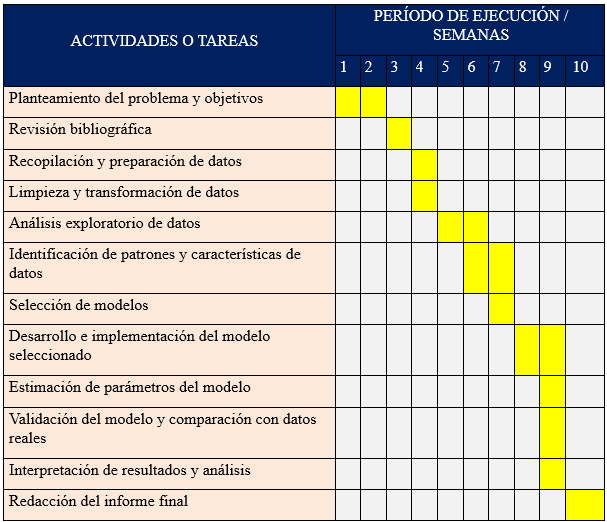
\includegraphics[width=0.9\textwidth]{2/figures/crono_activ.png}
				\caption{Cronograma de actividades}
				\textit{Fuente: Elaboración propia}
				\label{fig8}
			\end{center}	
		\end{figure}
		
		
		\begin{table}[h]
			\centering
			\caption{Presupuesto}
			\begin{tabular}{l|l|l|r}
				\textbf{Recurso} & \textbf{Categoria} & \textbf{Descripción} & \textbf{Costo (Soles)} \\ \hline
				Laptop & Equipo & Equipo de procesamiento del modelo de ML & 3000 \\
				Internet & Servicio & Servicio básico para el uso del estudio & 100\\
				Electricidad  & Servicio & Servicio básico para el uso del estudio  & 200\\
				Python & Software & Lenguaje de programación de alto nivel  & -\\
				Servicio en la nube & Servicio & Alojar backend & 100 \\
				Dominio web & Servicio & Dirección web personalizada & 50 \\
				Mantenimiento Sistema & Servicio & Ajustes, pruebas y monitoreo del sistema & 150 \\
				Almacenamiento nube & Servicio & Espacio virtual para respaldos del proyecto & 50 \\
				 \hline
			\end{tabular}
			\newline
			\newline
			\textit{Fuente: Elaboración propia}
			\label{tab:widgets}
		\end{table}
\chapter{DESARROLLO DEL EXPERIMENTO}
\section{Determinación y evaluación de alternativas de solución}

En primer lugar, se observó que la empresa cuenta con un amplio portafolio de productos, con más de 20 familias diferentes. Sin embargo, no todas estas familias tienen la misma relevancia en términos de ventas. Para abordar el desafío de predecir las ventas en este diverso conjunto de familias de productos, se llevó a cabo un proceso de selección cuidadoso. Se identificaron y seleccionaron las familias con mayor relevancia en las ventas, basándose en datos históricos y análisis de rendimiento comercial.

\begin{figure}[H]
	\begin{center}
		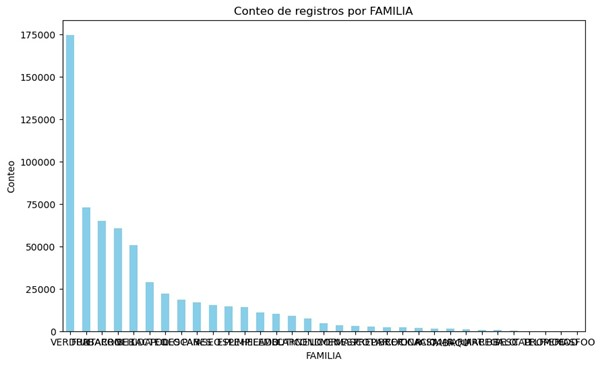
\includegraphics[width=0.9\textwidth]{2/figures/resul1_paper.jpg}
		\caption{Familia de productos}
		\textit{Fuente: Elaboración propia}
		\label{fig11}
	\end{center}
	
\end{figure}

Las familias de productos seleccionadas para el análisis representan una parte significativa de las operaciones comerciales de la empresa.  Se priorizaron  según  su  contribución  a los  ingresos  totales  y  su  impacto  en  la  rentabilidad  general.  Esta selección se basó en datos concretos, incluidos registros de ventas, análisis de tendencias del mercado y consultas con los departamentos de ventas y marketing. Con las familias de productos relevantes identificadas, se procedió a  explorar  diferentes  enfoques  para  predecir  las  ventas  futuras.  Se reconocieron dos alternativas principales, diseñadas para maximizar la utilidad de los datos disponibles y adaptarse a las necesidades específicas de cada familia de productos:



\begin{enumerate}
	\item Utilizar un Único Modelo de Predicción para las Familias Relevantes: En esta alternativa, se propone emplear un único modelo de predicción que abarque todas las familias de productos consideradas relevantes para las ventas. Este modelo se entrenaría utilizando datos históricos recopilados de estas familias y se utilizaría para realizar predicciones en tiempo real. Se considera que esta opción puede simplificar el proceso de predicción y ser más eficiente en términos de recursos y tiempo de implementación. No obstante, existe la preocupación de que este enfoque pueda subutilizar la información específica de cada familia, lo que podría resultar en predicciones menos precisas y adaptadas a las particularidades de cada una.
	
	\item Probar múltiples modelos para cada familia relevante: Esta alternativa implica la evaluación de varios modelos de predicción para cada familia de productos relevante en las ventas. Dado que la empresa cuenta con un amplio conjunto de familias de productos, se seleccionaron las seis más relevantes en términos de ventas. Se considera probar modelos como regresión logística, LSTM y XGBoost, entre otros, para determinar cuál proporciona las mejores métricas de rendimiento para cada familia. Aunque esta opción puede ser más compleja y requerir más recursos computacionales y tiempo de implementación, ofrece la ventaja de una mayor personalización y optimización para cada familia, lo que podría resultar en predicciones más precisas y adaptadas a sus características específicas.
\end{enumerate}



%\begin{table}
%	\centering
%	\begin{tabular}{l|r}
%		Item & Quantity \\\hline
%		Widgets & 42 \\
%		Gadgets & 13
%	\end{tabular}
%	\caption{\label{tab:widgets1}An example table.}
%\end{table}

\section{Propuesta solución}

Esta propuesta, como se explicó anteriormente, implica un enfoque más granular y específico para cada familia de productos seleccionada. En lugar de aplicar un único modelo de predicción a todas las familias, se explorará la idoneidad de múltiples modelos para cada una, teniendo en cuenta sus características individuales y su historial de ventas. Entre estos modelos se encuentran los siguientes:

\begin{itemize}
	\item \textbf{Linear Regression: } Un modelo de regresión lineal que busca la mejor relación lineal entre las variables independientes y la variable dependiente.
	\item \textbf{Decision Tree: } Un modelo basado en árboles de decisión que segmenta los datos en subconjuntos homogéneos.
	\item \textbf{Random Forest: } Un modelo de conjunto que utiliza múltiples árboles de decisión para mejorar la precisión de las predicciones.
	\item \textbf{Support Vector Regression (SVR): } Un modelo de regresión que utiliza máquinas de soporte vectorial para encontrar la mejor línea de ajuste en un espacio de características de alta dimensión.
	\item \textbf{XGBoost: } Un modelo de boosting de gradiente extremo que optimiza iterativamente los errores de predicción anteriores.
	\item \textbf{ARIMA: } Un modelo de series temporales que captura las dependencias auto-regresivas y de medias móviles.
	\item \textbf{LSTM: } Un tipo de red neuronal recurrente diseñada para manejar dependencias de largo plazo en series temporales.
	\item \textbf{Prophet: } Un modelo desarrollado por Facebook que se especializa en la predicción de series temporales con componentes estacionales y días festivos.
	
\end{itemize}

Todos estos modelos se entrenarán con la misma finalidad: determinar cuál es el más óptimo para realizar las predicciones de las ventas semanales de la familia de productos de verduras. Esta evaluación se llevará a cabo utilizando métricas de rendimiento como el Error Cuadrático Medio (MSE), la Raíz del Error Cuadrático Medio (RMSE), R2 Y (error porcentual absoluto medio) MAPE. Además, se considerará la capacidad de cada modelo para capturar patrones estacionales y tendencias a largo plazo presentes en los datos de ventas.


%%%%CAMBIO%%%%%%%%%555
\begin{figure}[H]
	\begin{center}
		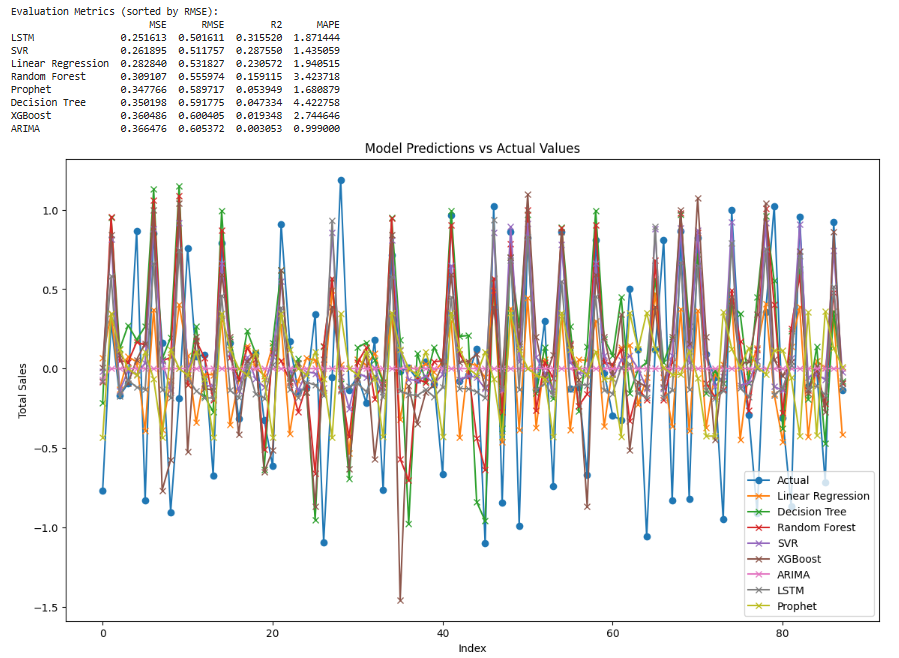
\includegraphics[width=0.9\textwidth]{2/figures/modelos_completo.png}
		\caption{Predicción Vs. valores actuales}
		\textit{Fuente: Elaboración propia}
		\label{fig11}
	\end{center}	
\end{figure}


\section{Planeamiento y descripción de actividades}
\subsection{Adquirir Base de Datos}
Este paso involucra obtener acceso a la base de datos de la empresa que contiene los registros históricos de ventas de las diferentes familias de productos. Se establecerá comunicación con los departamentos pertinentes para obtener los datos necesarios de manera segura y ética. En la Figura observamos que se adquiren las ventas desde el año 2023 al 2024, sumando más de 620 mil registros de ventas en este periodo.

\begin{figure}[H]
	\begin{center}
		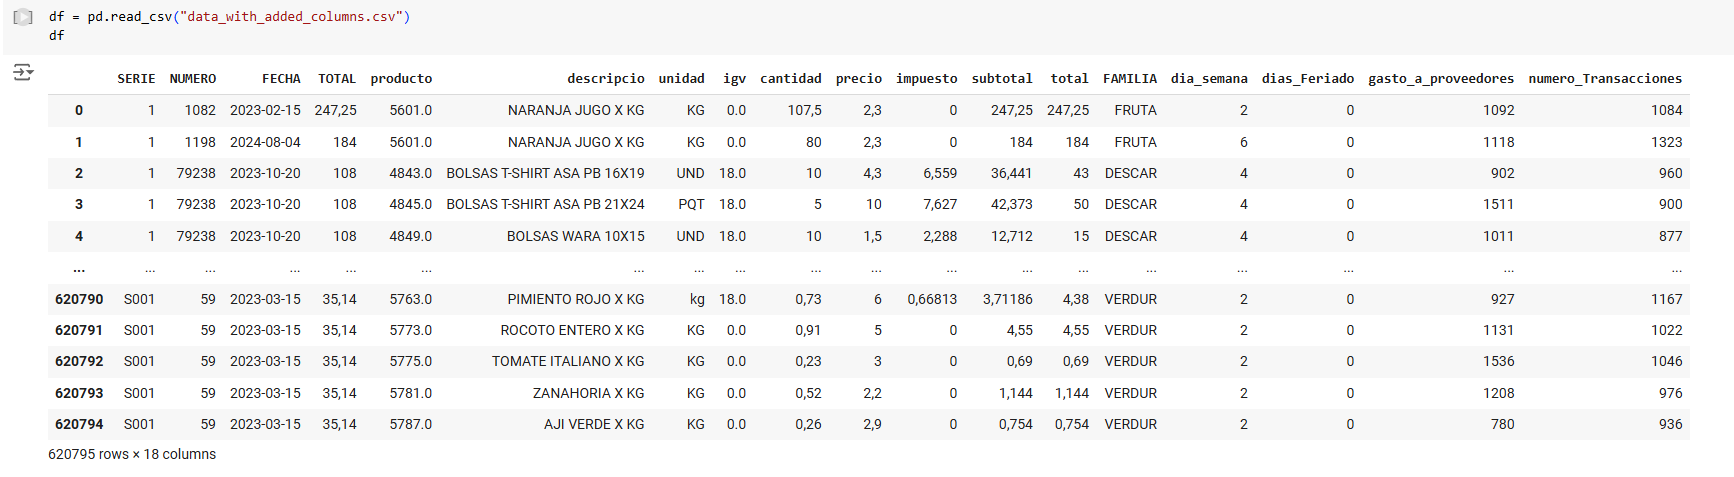
\includegraphics[width=0.9\textwidth]{2/figures/df_completa.png}
		\caption{Datos históricos de ventas}
		\textit{Fuente: Elaboración propia}
		\label{fig11}
	\end{center}	
\end{figure}

Posteriormente se decide agregar 3 nuevas columnas que serán relevantes para el pronostico de ventas. Siendo las columnas agregadas dias\_Feriado, 	gasto\_a\_proveedores y	numero\_Transacciones

\begin{figure}[H]
	\begin{center}
		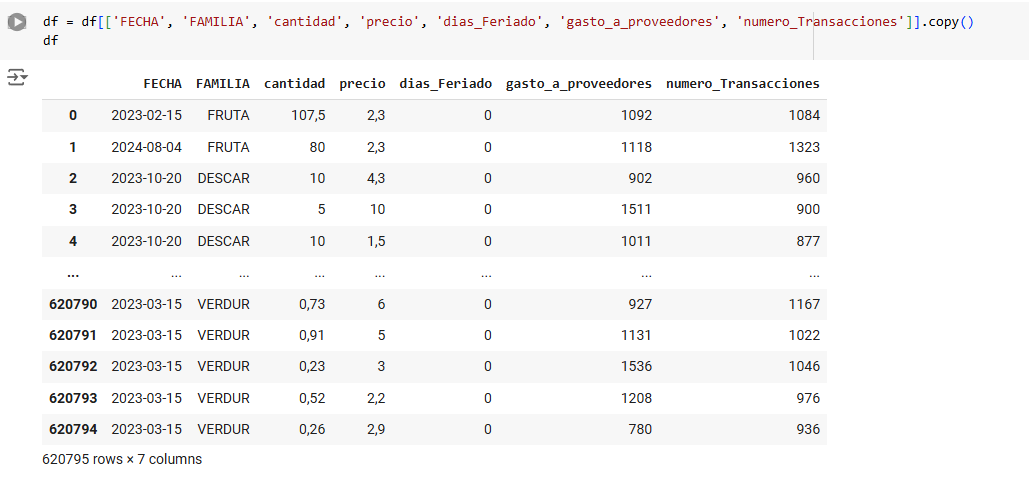
\includegraphics[width=0.9\textwidth]{2/figures/df_agregada.png}
		\caption{Datos históricos de ventas con 3 columnas agregadas}
		\textit{Fuente: Elaboración propia}
		\label{fig11}
	\end{center}	
\end{figure}


\subsection{Preprocesamiento de datos}
Antes de utilizar los datos para el análisis y modelado, es fundamental realizar un preprocesamiento adecuado. Esto incluye la limpieza de datos para eliminar valores faltantes o erróneos, la normalización para asegurar que todas las variables estén en la misma escala y la codificación de variables categóricas si es necesario. Adicional a estos pasos para asegurar la calidad, se decidio trabajar con la familia de Verduras para este analisis de Forecasting

\begin{figure}[H]
	\begin{center}
		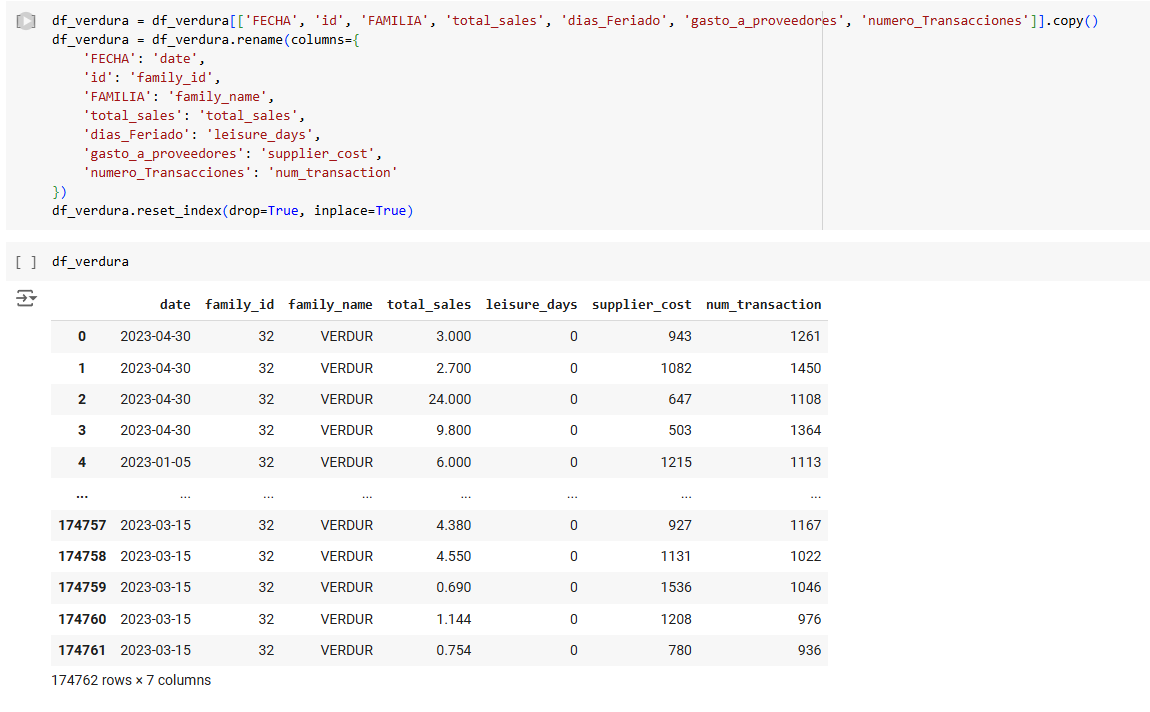
\includegraphics[width=0.9\textwidth]{2/figures/df_verduras_completa.png}
		\caption{Ventas de la familia verduras}
		\textit{Fuente: Elaboración propia}
		\label{fig11}
	\end{center}	
\end{figure}


\subsection{Selección de algoritmos a utilizar}
En este escenario, se han seleccionado los siguientes modelos para la predicción de ventas semanales de la familia de productos de verduras: Árbol de Decisión, Bosque Aleatorio, SVR, XGBoost, Regresión Lineal, ARIMA, LSTM y Prophet. Antes de proceder con el entrenamiento de estos modelos, se dividirán los datos en conjuntos de entrenamiento y prueba, asignando el 80\% de los datos para entrenamiento y el 20\% restante para pruebas.
\subsubsection{Proceso de Entrenamiento y Evaluación de Modelos}
\begin{enumerate}
	\item \textbf{División de Datos: } Los datos se dividirán en dos conjuntos:
		\begin{itemize}
			\item \textbf{Entrenamiento (80\%): } Utilizado para entrenar los modelos.
			\item \textbf{Prueba (20\%): } Utilizado para evaluar el rendimiento de los modelos.
		\end{itemize}
	\item \textbf{Entrenamiento de Modelos: } Cada uno de los modelos seleccionados se entrenará utilizando el conjunto de datos de entrenamiento. Este proceso implicará ajustar los parámetros de cada modelo para optimizar su rendimiento.
\end{enumerate}

\subsection{Definir parámetros}
Una vez seleccionados los modelos, se procederá a definir los parámetros iniciales de cada modelo y a realizar la optimización de hiperparámetros para mejorar su rendimiento predictivo. Esto se realizará utilizando técnicas como la búsqueda en cuadrícula o la optimización bayesiana. Una vez obteniendo estos parámetros se vera cual modelo es mejor para cada familia y se tomara la decisión de cual modelo trabajar con cada familia.

\begin{figure}[H]
	\begin{center}
		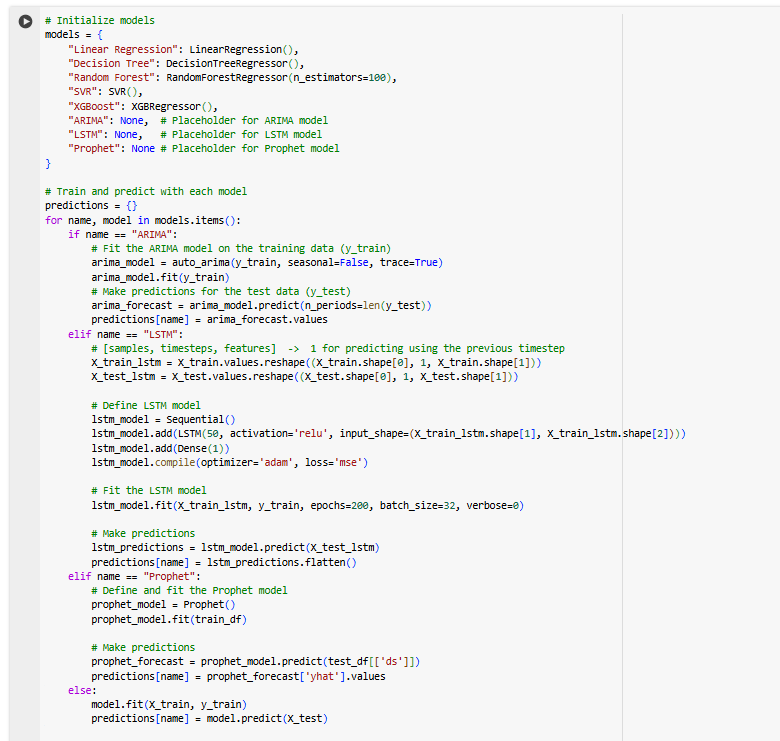
\includegraphics[width=0.9\textwidth]{2/figures/parametros_modelo.png}
		\caption{Parametros de los modelos elegidos}
		\textit{Fuente: Elaboración propia}
		\label{fig11}
	\end{center}	
\end{figure}


%
%\subsection{Obtener la predicción de cada Familia}
%Ya teniendo el modelo elegido para cada familia se comenzará a realizar la predicción para cada una de ellas y obtener las ventas futuras por semanas. Y una vez teniendo estos resultados se le brindara estos datos a los gerentes de empresa para que puedan hacerle uso a esta información.


\section{Desarrollo de actividades. Aplicación de herramientas de solución}

\subsection{Preprocesamiento de datos}
Se realizará un análisis exhaustivo para identificar y cuantificar los datos faltantes en el conjunto de datos históricos. Este análisis se llevará a cabo por columnas para determinar qué variables tienen valores ausentes y en qué medida.

%\subsection{Imputación de Datos Faltantes mediante KNN}
%Para abordar los valores faltantes identificados, se empleará el algoritmo de imputación de vecinos más cercanos (KNN). Este método permite predecir y completar los valores faltantes utilizando información de variables similares. Se seleccionará un número adecuado de vecinos para garantizar la precisión de la imputación.

%%%%%CAMBIO LISTO
\begin{figure}[H]
	\begin{center}
		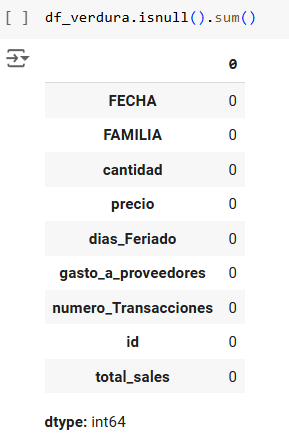
\includegraphics[width=0.4\textwidth]{2/figures/df_verdura_isnull.png}
		\caption{Identificando las columnas con datos faltantes}
		\textit{Fuente: Elaboración propia}
		\label{fig11}
	\end{center}	
\end{figure}

\subsection{Selección de Columnas relevantes}
Una vez completada la imputación de datos, se procederá a la selección de las columnas más relevantes para el análisis de predicción de ventas. En este caso, se considerarán las siguientes columnas como las más pertinentes:


%%%%%CAMBIO DE COLUMNAS LISTO
%%DATE, FAMLILY, TOTAL, LIISURE_DAYS,SUPPLIER, NUMTRANS

\begin{itemize}
	\item Date: Fecha de transacción de venta.
	\item Family\_id: Identificador unico del tipo de producto perecible
	\item Total: Medida principal de las ventas totales.
	\item Leisure\_days: Dia feriado por festividad gubernamental.
	\item Supplier\_cost: Número de pagos que se hicieron a proveedores en el día.
	\item Num\_transaction: Número de ventas en el día.
\end{itemize}
%%%CAMBIO LISSTO
\begin{figure}[H]
	\begin{center}
		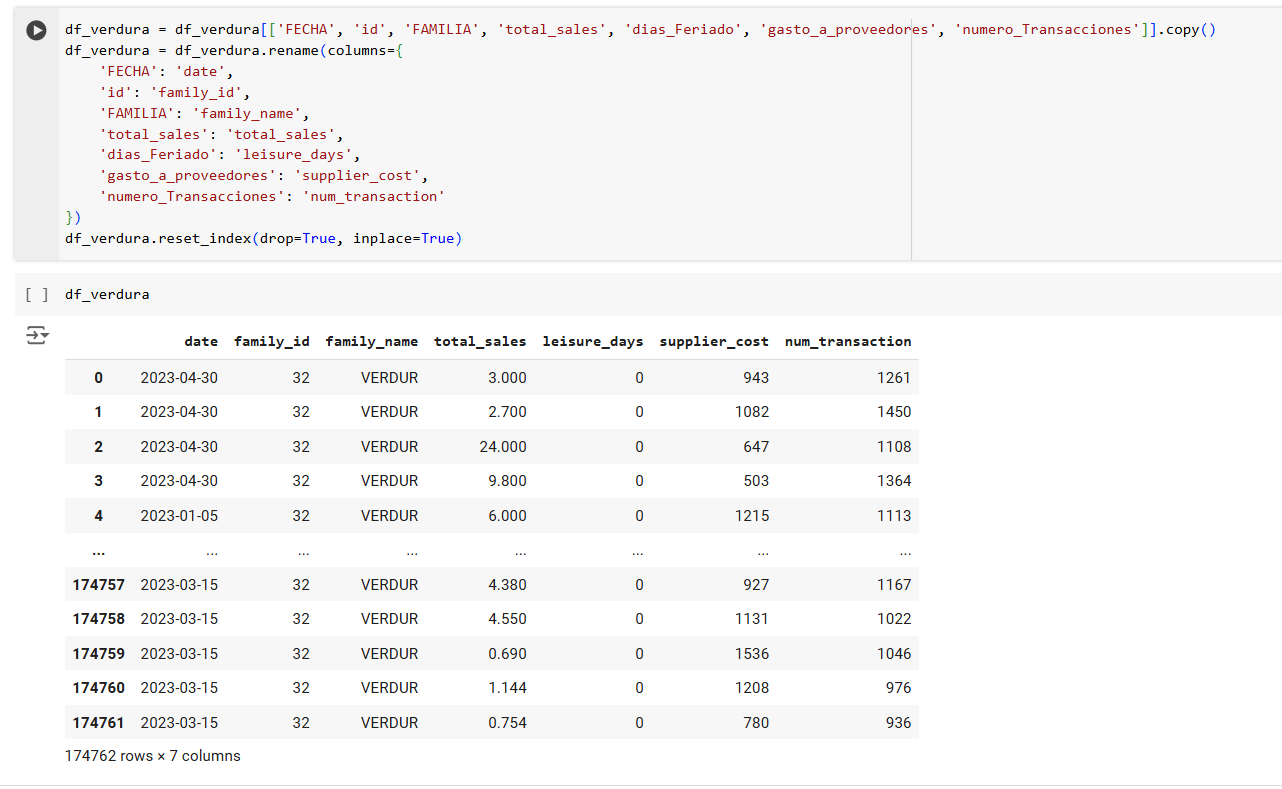
\includegraphics[width=0.7\textwidth]{2/figures/variables_dfverdura.png}
		\caption{Columnas de datos}
		\textit{Fuente: Elaboración propia}
		\label{fig11}
	\end{center}
	
\end{figure}
%%%CAMBIO LISTO
\begin{figure}[H]
	\begin{center}
		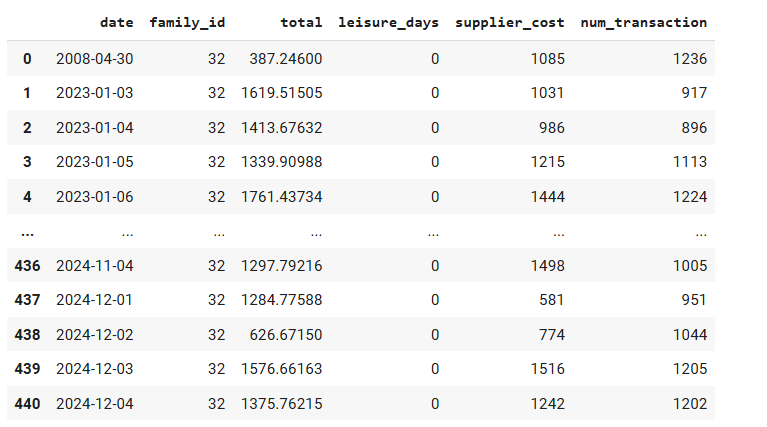
\includegraphics[width=0.7\textwidth]{2/figures/historico_ventas.png}
		\caption{Datos históricos de ventas}
		\textit{Fuente: Elaboración propia}
		\label{fig11}
	\end{center}
	
\end{figure}

\subsection{Seleccionamos los modelos a utilizar}
En este escenario, se han seleccionado los siguientes modelos: Árbol de Decisión, Random Forest, SVR, XGBoost y Regresión Lineal. Antes de proceder con el entrenamiento de estos modelos, se dividirá los datos en conjuntos de entrenamiento y prueba, asignando el 80\% de los datos para entrenamiento y el 20\% restante para pruebas.
%%CAMBIO LISTO

\begin{figure}[H]
	\begin{center}
		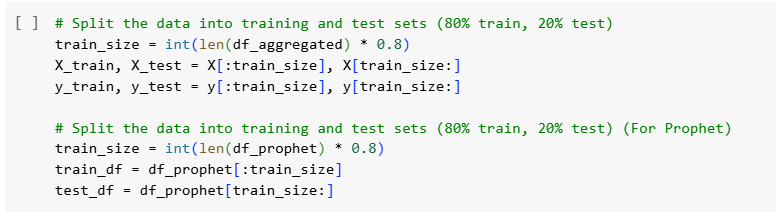
\includegraphics[width=0.7\textwidth]{2/figures/train_test.png}
		\caption{División de prueba y entrenamiento}
		\textit{Fuente: Elaboración propia}
		\label{fig11}
	\end{center}	
\end{figure}

\begin{figure}[H]
	\begin{center}
		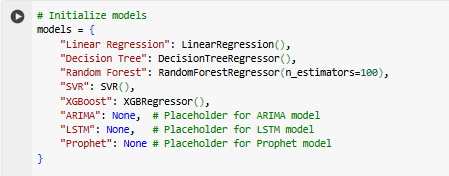
\includegraphics[width=0.7\textwidth]{2/figures/modelos.png}
		\caption{Modelos elegidos}
		\textit{Fuente: Elaboración propia}
		\label{fig11}
	\end{center}	
\end{figure}


A continuación se vera como se entrenan los modelos y las métricas que se eligieron que vendrían a ser RMSE, MSE, R2 y MAPE
%LISTO
\begin{figure}[H]
	\begin{center}
		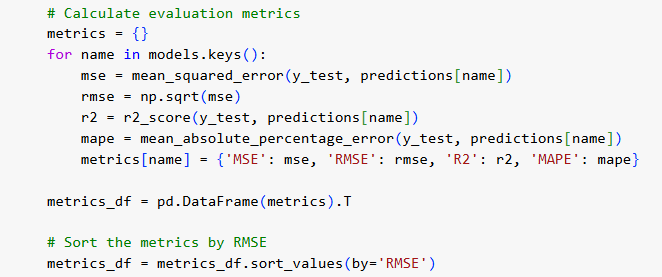
\includegraphics[width=0.7\textwidth]{2/figures/metricas_df.png}
		\caption{Definicion de modelos  y métricas}
		\textit{Fuente: Elaboración propia}
		\label{fig11}
	\end{center}
	
\end{figure}

%\begin{figure}[H]
%	\begin{center}
%		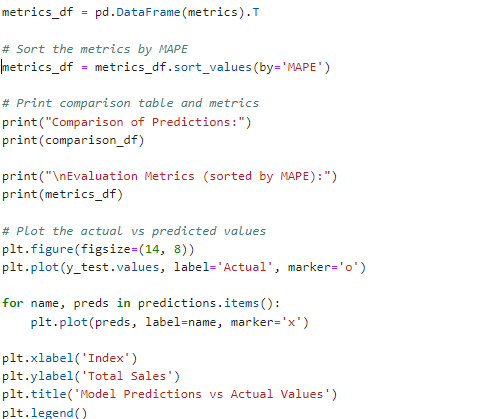
\includegraphics[width=0.7\textwidth]{2/figures/mape2.png}
%		\caption{}
%		\label{fig11}
%	\end{center}
%	
%\end{figure}

A continuación se vera la comparación de todos los modelos y apartir de eso se eligira el mejor modelo para trabajar con una familia.


\begin{figure}[H]
	\begin{center}
		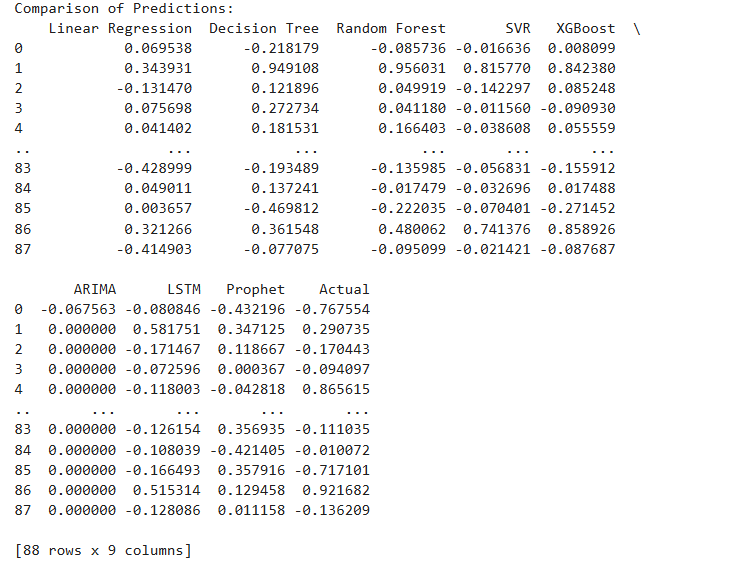
\includegraphics[width=0.8\textwidth]{2/figures/comparacion_modelos.png}
		\caption{Comparación de resultados}
		\label{fig22}
	\end{center}
	
\end{figure}


\begin{figure}[H]
	\begin{center}
		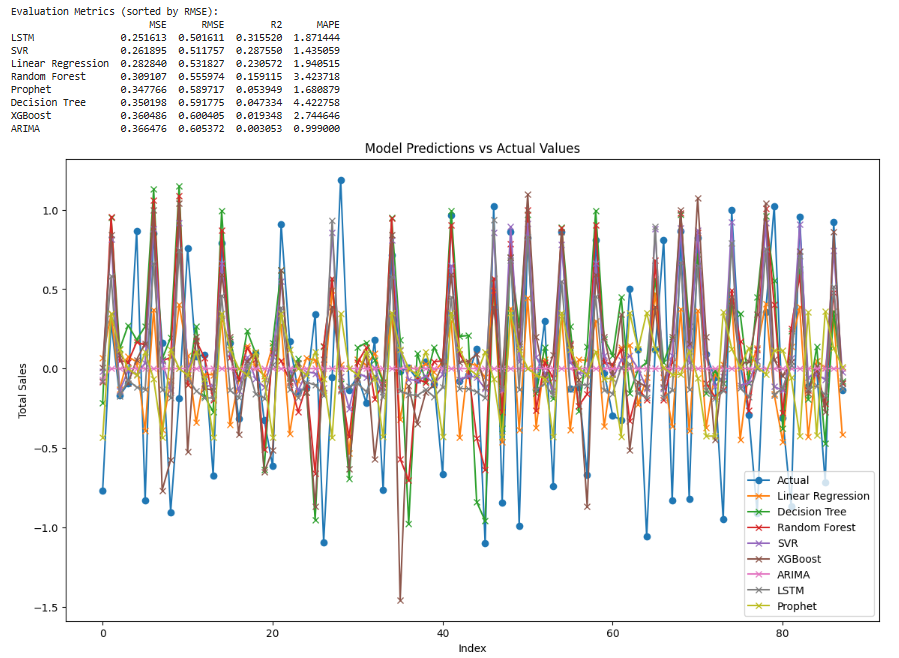
\includegraphics[width=0.8\textwidth]{2/figures/modelos_completo.png}
		\caption{Resultados de modelos}
		\label{fig23}
	\end{center}
	
\end{figure}
%
%\begin{figure}[H]
%	\begin{center}
%		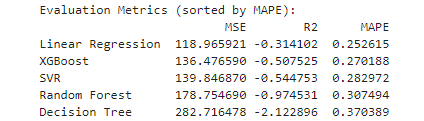
\includegraphics[width=0.7\textwidth]{2/figures/metricas.png}
%		\caption{}
%		\label{fig231}
%	\end{center}
%	
%\end{figure}



\section{Medición de la solución}
%%%%AGREGAR RMSE R2 LISTO
Los parámetros que se utilizaron para poder elegir el mejor modelo son los siguientes:

Raíz del error cuadrático medio (RMSE): El término utilizado para denotar el error que surge de la diferencia entre los valores predichos y los valores observados por un modelo o estimador es conocido como error cuadrático medio (RMSE). Esta medida se obtiene al calcular la raíz cuadrada de la media de los errores cuadráticos, lo cual refleja la disparidad entre los valores reales y los valores pronosticados. Es importante destacar que el RMSE, al ser siempre positivo, donde valores menores indican un ajuste más acertado de los datos al modelo. La formulación de este concepto se detalla en la siguiente sección.

\begin{equation}  
	\label{eq:RMSE}
	\hat{y}_i = \sqrt{\frac{\sum_{i=1}^{n} (y_i - \hat{y}_i)^2}{n}}
\end{equation}


Error Cuadrático Medio (MSE - Mean Squared Error): El MSE mide el promedio de los cuadrados de los errores entre las ventas reales y las ventas predichas por el modelo de regresión lineal. En otras palabras, indica cuán cerca están las ventas predichas de las ventas reales en términos de la diferencia cuadrada entre ellos.

\begin{equation}  
	\label{eq:MSE}
	\hat{\text{MSE} = \frac{1}{n} \sum_{i=1}^{n} (y_i - \hat{y}_i)^2
	}
\end{equation}

Error Porcentual Absoluto Medio (MAPE - Mean Absolute Percentage Error): El MAPE proporciona una medida de la precisión relativa del modelo de regresión lineal en términos porcentuales. Mide el promedio de los errores porcentuales absolutos entre las ventas reales y las ventas predichas. Esto te permite comprender cuánto se desvían, en promedio, las ventas predichas de las ventas reales en términos de porcentaje.

\begin{equation}  
	\label{eq:MAPE}
	\hat{\text{MAPE} = \frac{1}{n} \sum_{i=1}^{n} \left| \frac{y_i - \hat{y}_i}{y_i} \right| \times 100\%
	}
\end{equation}

Coeficiente de determinación: El valor del coeficiente de determinación (R2) oscila entre 0 y 1, reflejando la fracción de puntos en un conjunto de datos que se ajustan a la línea de regresión. Este coeficiente es una medida de la cantidad de variabilidad de la variable dependiente que puede ser explicada por el modelo de regresión. En el contexto de modelos estadísticos, R2 se emplea para predecir resultados futuros o validar hipótesis, siendo una herramienta crucial para evaluar la calidad del modelo y la proporción de variación en los resultados que este puede explicar. La formulación de R2 se presenta en la siguiente línea. (Bruce, P. et al. 2020)

\begin{equation}  
	\label{eq:r2}
	\hat{R}^2 = 1 - \frac{\sum_{i=1}^{n} (y_i - \hat{y}_i)^2}{\sum_{i=1}^{n}(y_i- \bar{y})^2}
\end{equation}



\subsection{Simulación de la predicción}
Se realizo la simulación a la familia que tiene más relevancia ósea “VERDURAS” como se menciono en el anterior punto se utilizo el modelo de regresión lineal ya que mostro mejores resultados en los parámetros RMSE, MSE ,R2 y MAPE. A continuación muestro el código con el que se trabajo para realizar la simulación de la predicción

%%CAMBIO 
\begin{figure}[H]
	\begin{center}
		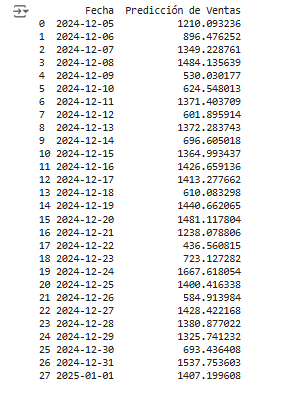
\includegraphics[width=0.5\textwidth]{2/figures/resultadofinal_numerico.png}
		\caption{Predicción numerica del mejor modelo}
		\textit{Fuente: Elaboración propia}
		\label{fig231}
	\end{center}	
\end{figure}


\begin{figure}[H]
	\begin{center}
		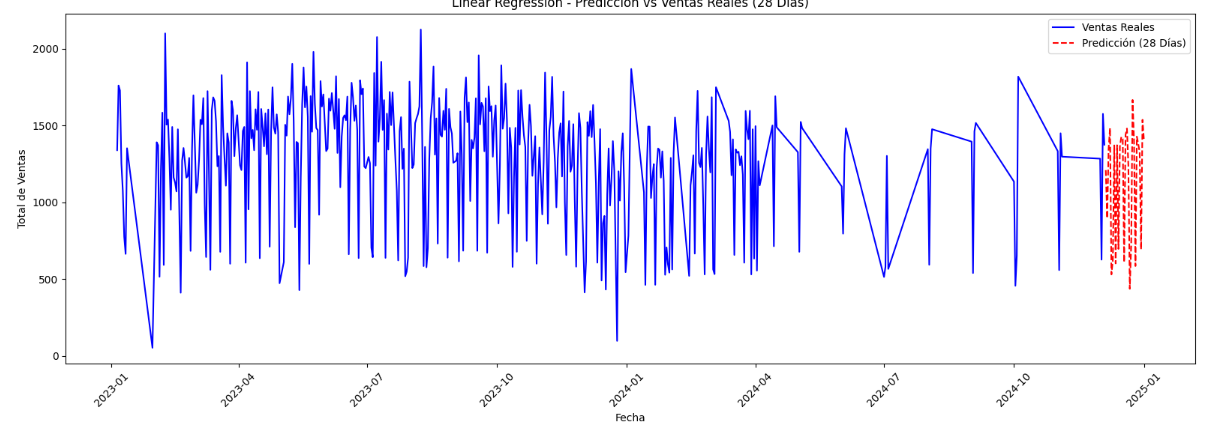
\includegraphics[width=0.9\textwidth]{2/figures/resultadofinal.png}
		\caption{Predicción con el mejor modelo}
		\textit{Fuente: Elaboración propia}
		\label{fig231}
	\end{center}	
\end{figure}



%En este código se utiliza Matplotlib para crear un gráfico que representa la predicción de ventas totales. Primero, se establece el tamaño de la figura. Luego, se trazan los datos de entrenamiento y prueba, así como las predicciones del mejor modelo. Se añade una línea vertical para indicar la división entre los conjuntos de entrenamiento y prueba. Y como resultado se obtiene:
%%%CAMBIO
%\begin{figure}[H]
%	\begin{center}
%		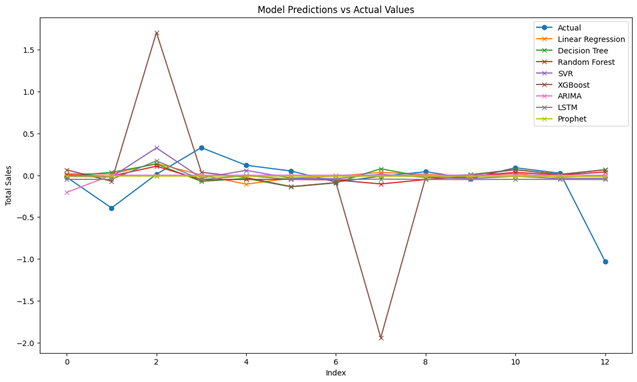
\includegraphics[width=0.9\textwidth]{2/figures/predict_Vs_actual.png}
%		\caption{Predicción Vs. valores actuales}
%		\textit{Fuente: Elaboración propia}
%		\label{fig11}
%	\end{center}	
%\end{figure}
\chapter{ANÁLISIS DE RESULTADOS}
\section{Resultados}

El presente capítulo tiene como finalidad analizar los resultados obtenidos a partir de la implementación de modelos predictivos aplicados a las ventas de la empresa \textbf{Market Dona}, enfocándose principalmente en la categoría de frutas. El propósito del estudio no solo fue obtener predicciones precisas de ventas, sino contribuir a la solución de uno de los principales problemas identificados en la empresa: el \textbf{sobrestock y la falta de stock de productos}.

Actualmente, Market Dona enfrenta dificultades relacionadas con la gestión de inventario debido a compras realizadas sin una estimación precisa de la demanda. Esta situación ocasiona dos escenarios negativos para la empresa. Por un lado, el exceso de productos genera sobrestock, incrementando pérdidas económicas por deterioro, especialmente en productos perecibles como las frutas. Por otro lado, una compra insuficiente provoca quiebres de stock, ocasionando pérdida de ventas y disminución de satisfacción en los clientes.

Frente a esta problemática, la investigación propone el uso de modelos predictivos como herramienta de apoyo para la toma de decisiones de compra. La finalidad es alcanzar un equilibrio adecuado entre la cantidad de productos adquiridos y la demanda real esperada. Para ello, se utilizó la predicción de ventas como base para elaborar un presupuesto de compra más preciso, permitiendo a Market Dona adquirir cantidades más cercanas a las necesidades reales del negocio.

De acuerdo con los resultados obtenidos, el modelo seleccionado como mejor alternativa fue \textbf{Linear Regression}, debido a que presentó los mejores indicadores de desempeño entre los modelos evaluados. Los resultados obtenidos fueron un \textbf{MAE de 399.57}, un \textbf{MSE de 279,381.62}, un \textbf{RMSE de 528.57} y un \textbf{$R^{2}$ de 0.744}.

El valor de \textbf{$R^{2} = 0.744$} indica que el modelo logra explicar aproximadamente el \textbf{74.4\% del comportamiento de las ventas}, lo que demuestra una capacidad adecuada para representar la tendencia de demanda en la categoría fruta. Esto es importante para Market Dona, ya que permite contar con estimaciones más confiables al momento de planificar las compras.

\begin{figure}
	\centering
	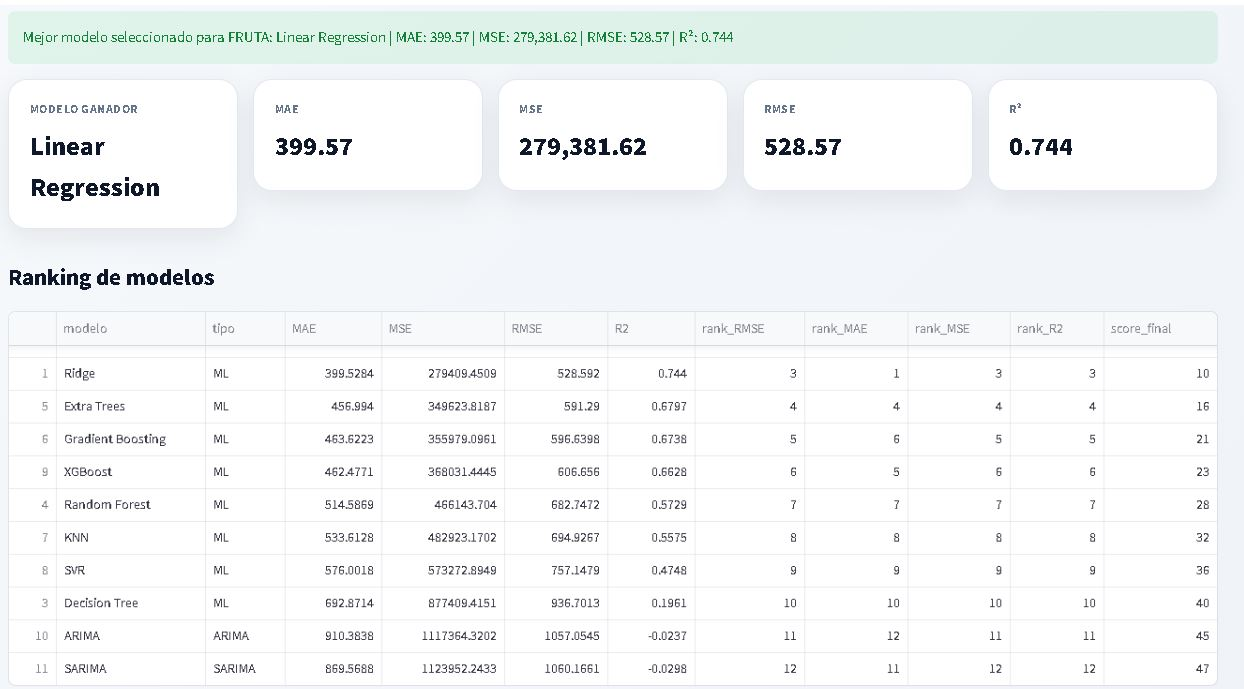
\includegraphics[width=0.8\textwidth]{4/Desa_ima/Propuestasol1.JPG}
	\caption{Gráfico de ventas reales vs predicción}
	\label{fig:real_vs_pred}
\end{figure}


Asimismo, el \textbf{MAE de 399.57} refleja que el margen promedio de error del modelo es relativamente bajo en comparación con el volumen general de ventas. Esto significa que las predicciones obtenidas pueden utilizarse como referencia válida para definir presupuestos de abastecimiento y reducir decisiones basadas únicamente en experiencia empírica o intuición.

En el gráfico de ventas reales versus predicción se observa que las predicciones mantienen un comportamiento cercano a las ventas reales durante gran parte del periodo evaluado. Aunque existen algunas diferencias en momentos de alta variabilidad, el modelo logra seguir la tendencia general del mercado. Este comportamiento resulta favorable para la empresa, debido a que permite anticipar cambios en la demanda y ajustar las compras de manera más eficiente.

Los resultados también evidencian que los modelos de Machine Learning obtuvieron un mejor desempeño que los modelos tradicionales de series temporales, como ARIMA y SARIMA. Estos últimos presentaron errores más elevados y valores negativos de $R^{2}$, lo cual indica una menor capacidad para representar el comportamiento real de las ventas. Esto sugiere que las ventas de Market Dona dependen no solo del tiempo, sino también de múltiples factores dinámicos que los modelos de aprendizaje automático pueden captar de mejor manera.

\begin{figure}
	\centering
	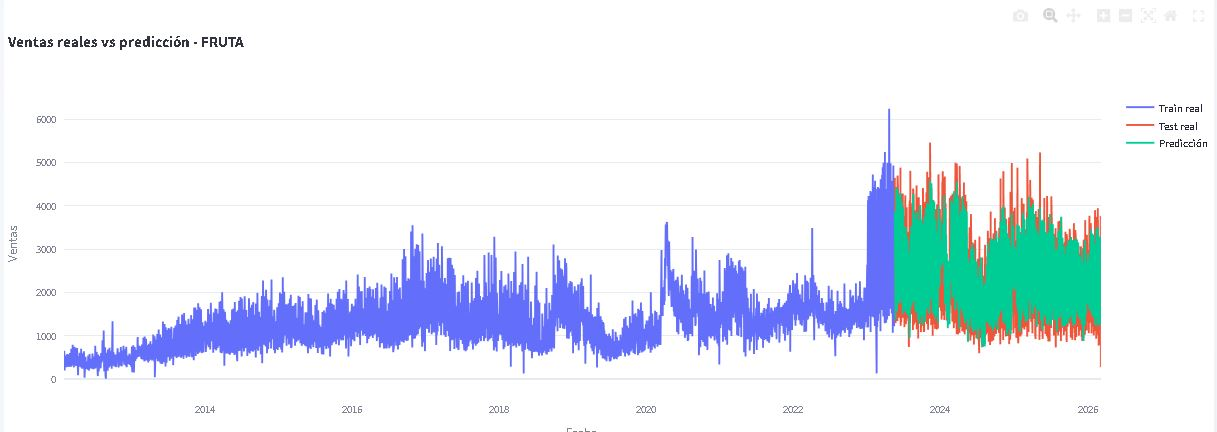
\includegraphics[width=0.9\textwidth]{4/Desa_ima/Propuestasol2.JPG}
	\caption{Gráfico de ventas reales vs predicción}
	\label{fig:real_vs_pred}
\end{figure}


La implementación de este sistema predictivo representa una mejora significativa para la gestión comercial de Market Dona. Mediante el uso de presupuestos basados en predicción de ventas, la empresa puede planificar mejor sus compras y mantener un equilibrio más adecuado entre oferta y demanda. Esto permite:

\begin{itemize}
    \item Reducir pérdidas ocasionadas por productos vencidos o deteriorados.
    \item Disminuir costos de almacenamiento innecesario.
    \item Evitar quiebres de stock y pérdida de clientes.
    \item Mejorar la disponibilidad de productos.
    \item Optimizar el uso del capital destinado a compras.
    \item Fortalecer la toma de decisiones basada en datos.
\end{itemize}

En términos prácticos, la predicción de ventas se convierte en una herramienta de apoyo para determinar cuánto comprar en cada periodo, evitando tanto compras excesivas como compras insuficientes. De esta manera, la empresa puede alcanzar un equilibrio de inventario que contribuya a mejorar su rentabilidad y eficiencia operativa.

Finalmente, los resultados demuestran que la aplicación de modelos predictivos en Market Dona puede contribuir significativamente a mejorar la gestión de inventario y el proceso de abastecimiento. El uso del modelo Linear Regression permitió obtener predicciones suficientemente precisas para apoyar la elaboración de presupuestos de compra, ayudando a reducir el sobrestock y minimizar la falta de productos, generando así un impacto positivo en las ventas y en la administración general de la empresa.



% A continuación de muestran los resultados obtenidos a partir de la metodología seguida. Estos resultados abarcan diferentes modelos de predicción como LSTM, Prophet, SVR, ARIMA, Linear Regression, Random Forest, Decision Tree, XGBoost. 

% \begin{enumerate}
% 	\item \textbf{LSTM (Long Short-Term Memory)}
% 		\begin{itemize}
% 			\item \textbf{Uso:} Redes neuronales recurrentes diseñadas para analizar datos secuenciales, como series temporales.
% 			\item \textbf{Escenarios: } Aplicaciones incluyen pronósticos de series temporales, procesamiento de lenguaje natural (NLP), y reconocimiento de voz.
% 			\item \textbf{Predictor: } Destacado por su capacidad para modelar patrones complejos y dependencias a largo plazo en datos de ventas.
% 		\end{itemize}
		
% 	\item \textbf{Prophet}
% 	\begin{itemize}
% 		\item \textbf{Uso: } Modelo de series temporales desarrollado por Facebook para prever datos con estacionalidad y tendencias cambiantes.
% 		\item \textbf{Escenarios: } Utilizado en pronósticos de ventas, gestión de inventarios y planificación de recursos.
% 		\item \textbf{Predictor: } Eficiente para capturar variaciones estacionales y cambios de tendencia en datos de ventas.
% 	\end{itemize}
	
% 	\item \textbf{SVR (Support Vector Regression)}
% 	\begin{itemize}
% 		\item \textbf{Uso: } Algoritmo de aprendizaje supervisado que encuentra un hiperplano óptimo en un espacio dimensional alto para la regresión.
% 		\item \textbf{Escenarios: } Aplicado en predicción de series temporales, análisis financiero y clasificación.
% 		\item \textbf{Predictor: } Efectivo cuando hay una separación clara entre los datos de ventas y se necesita evitar el sobreajuste.
% 	\end{itemize}
	
% 	\item \textbf{ARIMA (AutoRegressive Integrated Moving Average) }
% 	\begin{itemize}
% 		\item \textbf{Uso: } Modelo estadístico para analizar y pronosticar series temporales.
% 		\item \textbf{Escenarios: } Usado en pronóstico de demanda, análisis económico y finanzas.
% 		\item \textbf{Predictor: } Adecuado para datos de ventas con patrones estacionarios lineales o estacionales.
% 	\end{itemize}
	
% 	\item \textbf{Linear Regression}
% 	\begin{itemize}
% 		\item \textbf{Uso: } Modelo básico de regresión que asume una relación lineal entre variables.
% 		\item \textbf{Escenarios: } Aplicado en predicción de precios, análisis de mercado y evaluación de impacto.
% 		\item \textbf{Predictor: } Simple y rápido, útil cuando se requiere una interpretación clara de las relaciones entre variables.
% 	\end{itemize}
	
% 	\item \textbf{Random Forest}
% 	\begin{itemize}
% 		\item \textbf{Uso: } Método de aprendizaje en conjunto que combina múltiples árboles de decisión para mejorar la precisión.
% 		\item \textbf{Escenarios: } Utilizado en clasificación y regresión, detección de anomalías y análisis predictivo de marketing.
% 		\item \textbf{Predictor: } Eficiente para grandes conjuntos de datos con muchas variables, capturando relaciones no lineales.
% 	\end{itemize}
	
% 	\item \textbf{Decision Tree}
% 	\begin{itemize}
% 		\item \textbf{Uso: } Modelo que divide el conjunto de datos en subconjuntos más pequeños según características específicas.
% 		\item \textbf{Escenarios: } Aplicaciones en análisis de riesgos, diagnósticos médicos y segmentación de mercado.
% 		\item \textbf{Predictor: } Fácil de interpretar y visualizar, adecuado para datos estructurados y no estructurados.
% 	\end{itemize}
	
% 	\item \textbf{XGBoost (Extreme Gradient Boosting)}
% 	\begin{itemize}
% 		\item \textbf{Uso: } Algoritmo de aprendizaje en conjunto que utiliza árboles de decisión potenciados con gradientes.
% 		\item \textbf{Escenarios: } Utilizado en competiciones de Kaggle, pronóstico de series temporales, clasificación y regresión.
% 		\item \textbf{Predictor: } Potente para mejorar la precisión en grandes conjuntos de datos, especialmente en problemas complejos de predicción de ventas.
% 	\end{itemize}	
% \end{enumerate}


% %%%CAMBIO
% En la investigaación sobre la predicción de ventas en Market Donna, se evaluó varios modelos para determinar su eficacia. Tras analizar métricas como MSE, RMSE, R\textsuperscript{2} y MAPE, se encontró que el modelo de Regresión Lineal destacó como el mejor predictor entre los comparados. Con un MSE de 0.282840 y un RMSE de 0.531821, Regresión Lineal demostró una precisión superior en las predicciones en comparación con modelos como Prophet, SVR, ARIMA, LSTM, Random Forest, Decision Tree y XGBoost, los cuales mostraron métricas menos favorables. Este resultado destacó la capacidad de la regresion lineal para capturar patrones complejos en las series temporales de ventas de Market Donna, resaltando su relevancia en aplicaciones donde la exactitud en la predicción era crucial para la toma de decisiones estratégicas y operativas.


% %%CAMBIO
% \begin{table}[H]
% 	\centering
% 	\caption{Comparación de metricas}
% 	\begin{tabular}{lcccc}
% 		\hline
% 		& MSE      & RMSE     & R\textsuperscript{2}  & MAPE       \\ \hline
% 		LSTM                    & 0.253145 & 0.503135 & 0.311354 & 1.901903   \\
% 		Prophet                 & 0.347766 & 0.589717 & 0.053949 & 1.680879   \\
% 		SVR                     & 0.261895 & 0.511757 & 0.287550 & 1.435059   \\
% 		ARIMA                   & 0.366476 & 0.605372 & 0.003053 & 0.999000   \\
% 		Linear Regression       & 0.282840 & 0.531827 & 0.230572 & 1.940515   \\
% 		Random Forest           & 0.312075 & 0.558636 & 0.151043 & 3.434788   \\
% 		Decision Tree           & 0.350198 & 0.591775 & 0.047334 & 4.422758   \\
% 		XGBoost                 & 0.360486 & 0.600405 & 0.019348 & 2.744646  \\ \hline
% 	\end{tabular}
% 	\newline
% 	\newline \textit{Fuente: Elaboración propia}
% 	\label{table:models_comparison}
% \end{table}



%\section{Y}
%
%Nisi porta lorem mollis aliquam ut porttitor leo. Aenean pharetra magna ac placerat vestibulum. Est placerat in egestas erat imperdiet sed euismod. Velit euismod in pellentesque massa placerat. Enim praesent elementum facilisis leo vel fringilla. Ante in nibh mauris cursus mattis molestie a iaculis. Erat pellentesque adipiscing commodo elit at imperdiet dui accumsan sit. Porttitor lacus luctus accumsan tortor posuere ac ut. Tortor at auctor urna nunc id. A iaculis at erat pellentesque adipiscing commodo elit. 
%
%
%\section{Z}
%
%Nisi porta lorem mollis aliquam ut porttitor leo. Aenean pharetra magna ac placerat vestibulum. Est placerat in egestas erat imperdiet sed euismod. Velit euismod in pellentesque massa placerat. Enim praesent elementum facilisis leo vel fringilla. Ante in nibh mauris cursus mattis molestie a iaculis. Erat pellentesque adipiscing commodo elit at imperdiet dui accumsan sit. Porttitor lacus luctus accumsan tortor posuere ac ut. Tortor at auctor urna nunc id. A iaculis at erat pellentesque adipiscing commodo elit.

\chapter{CONCLUSIONES}
%\section{Conclusiones}

Se concluye que la implementación de un modelo predictivo de demanda contribuye a mejorar la toma de decisiones en el proceso de pedido a proveedores en Donna S.A.C., debido a que permite estimar la demanda futura de productos perecibles a partir de datos históricos de ventas y variables temporales relevantes. De esta manera, la empresa puede contar con una herramienta de apoyo para planificar el reabastecimiento con mayor precisión, reduciendo la dependencia de decisiones basadas únicamente en la experiencia o criterios subjetivos.

Respecto al primer objetivo específico, se determinó que la calidad de la base de datos histórica influye directamente en la precisión de los modelos predictivos. La disponibilidad de registros organizados, completos y consistentes permitió construir una serie temporal adecuada para el análisis de la demanda. Asimismo, la identificación de valores atípicos, datos duplicados o inconsistencias fue necesaria para evitar distorsiones en el entrenamiento del modelo y mejorar la confiabilidad de los resultados obtenidos.

En relación con el segundo objetivo específico, se concluye que las técnicas de preprocesamiento de datos fueron fundamentales para mejorar el rendimiento de los modelos de predicción. La limpieza de datos, la agrupación diaria de ventas, el tratamiento de valores atípicos, la selección de columnas relevantes y la construcción de variables temporales permitieron transformar los registros históricos en una base adecuada para el modelamiento predictivo. Estas actividades fortalecieron la capacidad del modelo para identificar patrones de comportamiento en la demanda de productos perecibles.

Con respecto al tercer objetivo específico, se identificó que las variables temporales e históricas tienen una influencia relevante en el comportamiento de la demanda. Factores como el día de la semana, el mes, las ventas históricas, los rezagos de demanda y los promedios móviles permitieron representar mejor las variaciones de consumo. Esto confirma que la demanda de productos perecibles no presenta un comportamiento uniforme, sino que responde a patrones temporales que deben ser considerados en el proceso de pronóstico.

En cuanto al cuarto objetivo específico, se evaluaron distintos modelos de forecasting y machine learning mediante métricas como MAE, MSE, RMSE, MAPE y R$^2$. A partir de esta comparación, se seleccionó el modelo con mejor desempeño predictivo y mayor aplicabilidad para el contexto de la empresa. Según los resultados obtenidos, el modelo seleccionado presentó una capacidad adecuada para aproximarse a la demanda real, por lo que puede ser utilizado como apoyo para la planificación de compras y la optimización del reabastecimiento.

Finalmente, se concluye que la propuesta desarrollada representa una mejora metodológica y operativa para Donna S.A.C., ya que permite convertir los datos históricos de ventas en información útil para la toma de decisiones. La implementación del modelo predictivo no solo aporta a la estimación de la demanda futura, sino que también contribuye a reducir riesgos asociados al sobrestock, quiebres de stock y pérdidas por productos perecibles, fortaleciendo así la eficiencia del proceso de abastecimiento.




%%%%%CAMBIO
% Se puede concluir que el desarrollo de modelos predictivos de demanda, utilizando técnicas avanzadas como Regresión Lineal Multiple, es esencial para mejorar la rentabilidad en la venta de productos perecibles. Integrar datos históricos de ventas con variables clave como feriados, pago proveedores y precios no solo facilita una gestión de inventario más precisa, sino que también optimiza las estrategias de precios y promociones, lo que resulta en una planificación más efectiva y en un aumento de la rentabilidad.

% La investigación enfocada en modelos de Forecasting para maximizar la planificación de recursos en Donna S.A.C. destaca la importancia de recopilar datos detallados sobre el desempeño de ventas en diversas áreas y períodos. Estos datos son cruciales para identificar patrones de comportamiento de los clientes, evaluar el impacto de estrategias comerciales variadas y anticipar cambios en la demanda. La implementación adecuada de modelos de Forecasting no solo facilita la predicción precisa de ventas futuras, sino que también proporciona valiosos insights para la toma de decisiones estratégicas que impulsan el crecimiento sostenido de la empresa.

% El análisis de modelos de Forecasting, al considerar la estructura temporal de los datos y factores como tendencias, estacionalidad y variación aleatoria, permite la aplicación de modelos estadísticos avanzados para pronosticar con precisión el comportamiento futuro de las ventas. Este enfoque es fundamental para empresas como Donna S.A.C., donde la capacidad de prever la demanda de manera confiable puede marcar la diferencia en la planificación operativa y estratégica. Así, el uso efectivo de modelos de Forecasting no solo mejora la eficiencia en la gestión de recursos, sino que también fortalece la capacidad de la empresa para adaptarse ágilmente a cambios en el mercado y maximizar su rentabilidad.


%
%
%
%\section{Recomendaciones}
%
%Nisi porta lorem mollis aliquam ut porttitor leo. Aenean pharetra magna ac placerat vestibulum. Est placerat in egestas erat imperdiet sed euismod. Velit euismod in pellentesque massa placerat. Enim praesent elementum facilisis leo vel fringilla. Ante in nibh mauris cursus mattis molestie a iaculis. Erat pellentesque adipiscing commodo elit at imperdiet dui accumsan sit. Porttitor lacus luctus accumsan tortor posuere ac ut. Tortor at auctor urna nunc id. A iaculis at erat pellentesque adipiscing commodo elit. 



	
	
	%%Anexos
	\appendix
	\renewcommand{\appendixname}{Anexos}
	\renewcommand{\appendixtocname}{Anexos}
	\renewcommand{\appendixpagename}{Anexos}
	\clearpage
	\addappheadtotoc
	\appendixpage
	% \clearpage
\section*{\huge Anexo I: Matriz de Consistencia}
% \addcontentsline{toc}{section}{Anexo I: Matriz de Consistencia}
	\begin{table}[H]
		\centering
		\small
		\begin{tabular}{ |m{5cm}|m{5cm}|m{5cm}|  }
			\hline
			\rowcolor{bluejean}
			\Centering \color{white}{PROBLEMAS}& \Centering \color{white}{OBJETIVOS}& \Centering \color{white}{HIPÓTESIS}\\
			\hline
			\rowcolor{turq}
			\Centering Problema General& \Centering Objetivo General & \Centering Hipótesis General \\
			\hline
			{\ProblemaGeneral} & { \ObjetivoGeneral} & {\HipotesisGeneral} \\
			\hline
			\rowcolor{turq}
			\Centering Problemas Específicos& \Centering Objetivos Específicos & \Centering Hipótesis Específicas \\
			\hline
			{\Pbone} & {\Objone} & {\Hone} \\
			\hline
			{\Pbtwo} & {\Objtwo} & {\Htwo} \\
			\hline
			{\Pbthree} & {\Objthree} & {\Hthree} \\
			\hline
			% {\Pbfour} & {\Objfour} & {\Hfour} \\
			% \hline
	%		{\Pbfive} & {\Objfive} & {\Hfive} \\
	%		\hline
		\end{tabular}
		\caption{Matriz de consistencia}
		
		\label{1:table}
	\end{table}


\section*{\huge Anexo II: Arquitectura de Software}
\vspace{-2cm}
	\begin{figure}[H]
		\centering
		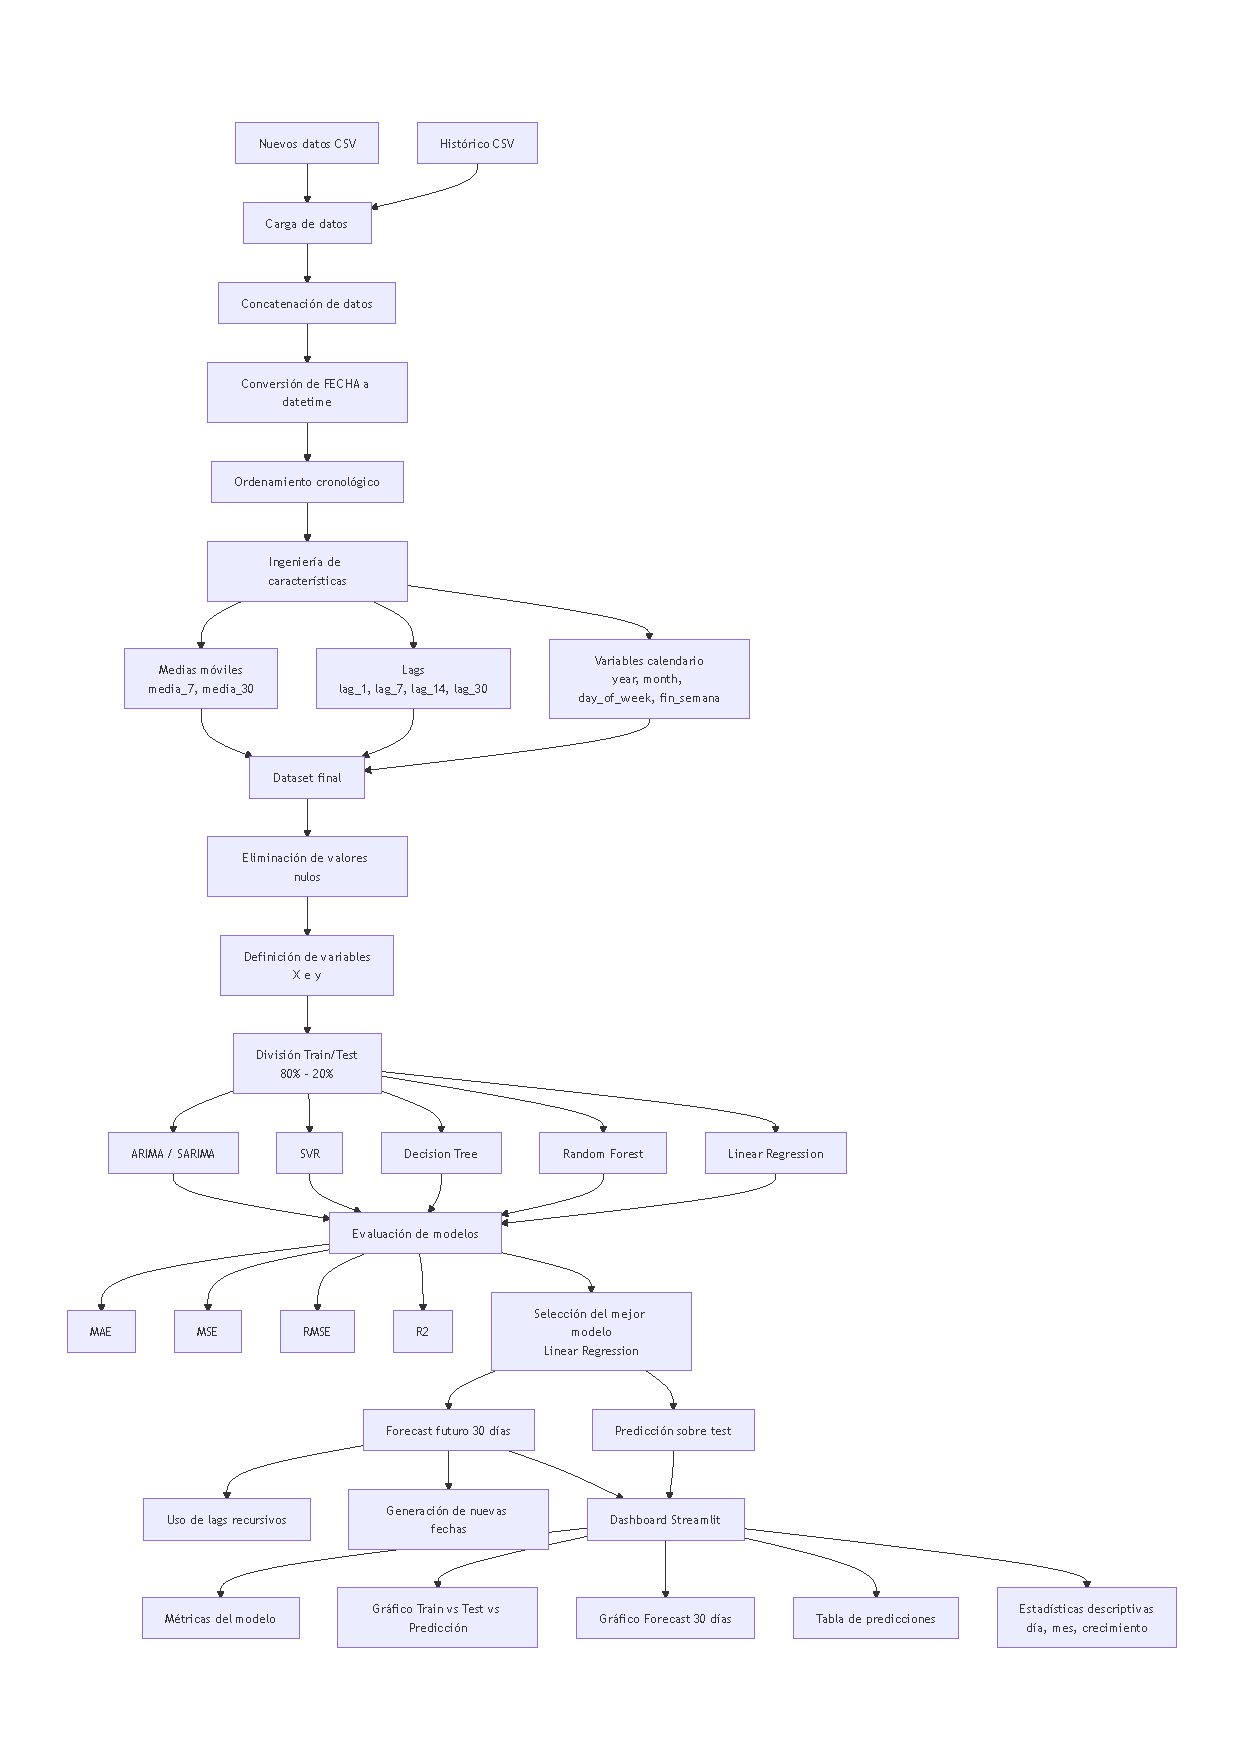
\includegraphics[width=1.05\textwidth]{anexos/arquitectura.pdf}
		\caption{Arquitectura de Software}
		\label{fig:arquitectura}
	\end{figure}


\section*{\huge Anexo III: Estados Financieros}


%%%%%%%%%%%%%%%%%%%%%%%%%%%%%%%%%%%%%%%%%%%%%%%%%%%%%%%%%%%%%%%%%%%%%%%
\subsection*{ESTADO DE GANANCIAS Y PÉRDIDAS (ENERO 2026)}

\begin{table}[H]
	\centering
	\begin{tabular}{|L{8cm}|R{4cm}|}
	\hline
	\rowcolor{yellow} LOCAL: & \cellcolor{purple!30} SAMOA \\ 
	\rowcolor{black}\textcolor{white}{PERIODO:} & \textcolor{white}{Ene-26} \\ \hline
	\rowcolor{yellow} VENTAS ORION & 273,126.10 \\ 
	\textcolor{red}{COSTO DE MERCAD VENDIDA} & 198,915.12 \\ 
	\rowcolor{gray!30} MARGEN COMERCIAL & 74,210.98 \\ 
	MERMAS & 641.27 \\ 
	PERDIDAS & 753.80 \\ 
	\rowcolor{gray!30} MARGEN BRUTO & 72,815.91 \\ 
	RRHH TIENDA & 23,886.95 \\ 
	RRHH CENTRAL & 2,183.75 \\ 
	GASTO DE COMPRA & 1,219.90 \\ 
	GASTOS DE VENTAS & 3,225.93 \\ 
	COMISION POS & 5,192.28 \\ 
	GASTO DE MKT & 152.00 \\ 
	PAGO DE SERVICIOS & 3,309.20 \\ 
	COSTOS DE LOCACION & 4,504.88 \\ 
	GASTOS FINANCIEROS & 142.21 \\ 
	\rowcolor{yellow} EBITDA & 29,283.23 \\ 
	PAGO DEUDAS & - \\ 
	INVERSIONES & 33,000.00 \\ 
	\rowcolor{yellow} EBIT & (3,716.77) \\ 
	IMPUESTOS & 2,993.40 \\ 
	\rowcolor{yellow} BENEFICIOS NETOS & (6,710.17) \\ \hline
	\end{tabular}
\caption{Fuente: Elaboración propia}
\end{table}

\vspace{1cm} % espacio entre tablas


\subsection*{FLUJO DE CAJA (ENERO 2026)}

\begin{table}[H]
	% \caption{Flujo de Caja (Tabla 1.3)}
	\centering
	\begin{tabular}{|L{8cm}|R{4cm}|}
	\hline
	\rowcolor{green!30} LOCAL: & \cellcolor{purple!30} SAMOA \\
	\rowcolor{black}\textcolor{white}{PERIODO:} & \textcolor{white}{Ene-26} \\ \hline
	SALDO INI y/o ANT & \\ 
	APALANCAMIENTO / PRESTAMOS & \\ 
	\rowcolor{green!30} VENTAS ORION & 273,126.10 \\ 
	PAGO POR MERCADERIAS & 191,255.72 \\ 
	RRHH TIENDA & 23,886.95 \\ 
	RRHH CENTRAL & 2,183.75 \\ 
	GASTO DE COMPRA & 1,219.90 \\ 
	GASTOS DE VENTAS & 3,225.93 \\ 
	COMISION POS & 5,192.28 \\ 
	GASTO DE MKT & 152.00 \\ 
	PAGO DE SERVICIOS & 3,309.20 \\ 
	COSTOS DE LOCACION & 4,504.88 \\ 
	GASTOS FINANCIEROS & 142.21 \\ 
	PAGO DE DEUDAS & - \\ 
	INVERSIONES & 33,000.00 \\ 
	IMPUESTOS & 2,993.40 \\ 
	\rowcolor{green!30} EGRESOS TOTAL & 271,066.22 \\ 
	\rowcolor{yellow} FLUJO DE CAJA & 2,059.88 \\ \hline
	\end{tabular}
\caption{Fuente: Elaboración propia}
\end{table}

Descripcion:

En enero 2026, la tienda \textbf{Samoa} tuvo ventas de \textbf{S/ 273,126.10} con un margen bruto de \textbf{S/ 72,815.91}. El \textbf{EBITDA} fue de \textbf{S/ 29,283.23}, aunque tras inversiones de \textbf{S/ 33,000} y otros gastos, el \textbf{EBIT} quedó negativo en \textbf{(S/ 3,716.77)}, resultando en una pérdida neta de \textbf{(S/ 6,710.17)}. El flujo de caja fue positivo en \textbf{S/ 2,059.88}, indicando que a pesar de los resultados contables negativos, las operaciones generaron liquidez suficiente para cubrir los compromisos inmediatos.

%%%%%%%%%%%%%%%%%%%%%%%%%%%%%%%%%%%%%%%%%%%%%%%%%%%%%%%%%%%%%%%%
\subsection*{ESTADO DE GANANCIAS Y PÉRDIDAS (FEBRERO 2026)}

%=====================
\begin{table}[H]
\centering
% \caption{Estado de Ganancias y Pérdidas (Tabla 1.4)}
\begin{tabular}{|L{8cm}|R{4cm}|}
\hline
\rowcolor{yellow} LOCAL: & \cellcolor{purple!30} SAMOA \\ 
\rowcolor{black}\textcolor{white}{PERIODO:} & \textcolor{white}{Feb-24} \\ \hline
\rowcolor{yellow} VENTAS ORION & 255,282.10 \\ 
\textcolor{red}{COSTO DE MERCAD VENDIDA} & 180,542.02 \\ 
\rowcolor{gray!30} MARGEN COMERCIAL & 74,740.08 \\ 
MERMAS & 1,693.47 \\ 
PERDIDAS & 178.30 \\ 
\rowcolor{gray!30} MARGEN BRUTO & 72,868.31 \\ 
RRHH TIENDA & 22,124.69 \\ 
RRHH CENTRAL & 2,783.75 \\ 
GASTO DE COMPRA & 1,342.50 \\ 
GASTOS DE VENTAS & 3,488.70 \\ 
COMISION POS & 4,886.10 \\ 
GASTO DE MKT & - \\ 
PAGO DE SERVICIOS & 3,724.80 \\ 
COSTOS DE LOCACION & - \\ 
GASTOS FINANCIEROS & 28.50 \\ 
\rowcolor{yellow} EBITDA & 34,546.27 \\ 
PAGO DEUDAS & - \\ 
INVERSIONES & 15,263.49 \\ 
\rowcolor{yellow} EBIT & 19,282.78 \\ 
IMPUESTOS & 2,812.20 \\ 
\rowcolor{yellow} BENEFICIOS NETOS & 16,470.58 \\ \hline
\end{tabular}
\caption{Fuente: Elaboración propia}
\end{table}

\vspace{1cm}

%=====================
\subsection*{FLUJO DE CAJA (FEBRERO 2026)}

\begin{table}[H]
\centering
% \caption{Flujo de Caja (Tabla 1.5)}
\begin{tabular}{|L{8cm}|R{4cm}|}
\hline
\rowcolor{green!30} LOCAL: & \cellcolor{purple!30} SAMOA \\
\rowcolor{black}\textcolor{white}{PERIODO:} & \textcolor{white}{Feb-24} \\ \hline
SALDO INI y/o ANT & \\ 
APALANCAMIENTO / PRESTAMOS & \\ 
\rowcolor{green!30} VENTAS ORION & 255,282.10 \\ 
PAGO POR MERCADERIAS & 184,699.99 \\ 
RRHH TIENDA & 22,124.69 \\ 
RRHH CENTRAL & 2,783.75 \\ 
GASTO DE COMPRA & 1,342.50 \\ 
GASTOS DE VENTAS & 3,488.70 \\ 
COMISION POS & 4,886.10 \\ 
GASTO DE MKT & - \\ 
PAGO DE SERVICIOS & 3,724.80 \\ 
COSTOS DE LOCACION & - \\ 
GASTOS FINANCIEROS & 28.50 \\ 
PAGO DE DEUDAS & - \\ 
INVERSIONES & 15,263.49 \\ 
IMPUESTOS & 2,812.20 \\ 
\rowcolor{green!30} EGRESOS TOTAL & 241,154.72 \\ 
\rowcolor{yellow} FLUJO DE CAJA & 14,127.38 \\ \hline
\end{tabular}
\caption{Fuente: Elaboración propia}
\end{table}

Descripcion:

En febrero 2026, las ventas descendieron a \textbf{S/ 255,282.10}, pero el margen bruto se mantuvo estable en \textbf{S/ 72,868.31}. El \textbf{EBITDA} subió a \textbf{S/ 34,546.27} y el \textbf{EBIT} fue de \textbf{S/ 19,282.78}, generando beneficios netos de \textbf{S/ 16,470.58}. El flujo de caja mejoró significativamente a \textbf{S/ 14,127.38}, reflejando un manejo más eficiente de los costos y una recuperación de liquidez, lo que indica un mejor control en la planificación de compras y mermas.

%%%%%%%%%%%%%%%%%%%%%%%%%%%%%%%%%%%%%%%%%%%%%%%%%%%%%%%%%%%%%%%%%%%%%%%%%%%%
\subsection*{ESTADO DE GANANCIAS Y PÉRDIDAS (MARZO 2026)}

\begin{table}[H]
\centering
% \caption{Estado de Ganancias y Pérdidas (Tabla 1.6)}
\begin{tabular}{|L{8cm}|R{4cm}|}
\hline
\rowcolor{yellow} LOCAL: & \cellcolor{purple!30} SAMOA \\ 
\rowcolor{black}\textcolor{white}{PERIODO:} & \textcolor{white}{Mar-24} \\ \hline
\rowcolor{yellow} VENTAS ORION & 276,817.65 \\ 
\textcolor{red}{COSTO DE MERCAD VENDIDA} & 198,176.69 \\ 
\rowcolor{gray!30} MARGEN COMERCIAL & 78,640.96 \\ 
MERMAS & - \\ 
PERDIDAS & 468.30 \\ 
\rowcolor{gray!30} MARGEN BRUTO & 78,172.66 \\ 
RRHH TIENDA & 27,444.76 \\ 
RRHH CENTRAL & 4,527.01 \\ 
GASTO DE COMPRA & 1,182.00 \\ 
GASTOS DE VENTAS & 3,945.50 \\ 
COMISION POS & 5,497.56 \\ 
GASTO DE MKT & 400.00 \\ 
PAGO DE SERVICIOS & 3,392.80 \\ 
COSTOS DE LOCACION & - \\ 
GASTOS FINANCIEROS & 28.50 \\ 
\rowcolor{yellow} EBITDA & 31,811.53 \\ 
PAGO DEUDAS & - \\ 
INVERSIONES & 14,480.33 \\ 
\rowcolor{yellow} EBIT & 17,331.20 \\ 
IMPUESTOS & 1,578.25 \\ 
\rowcolor{yellow} BENEFICIOS NETOS & 15,752.95 \\ \hline
\end{tabular}
\caption{Fuente: Elaboración propia}
\end{table}

\vspace{1cm}

%=====================
\subsection*{FLUJO DE CAJA (MARZO 2026)}
\begin{table}[H]
\centering
% \caption{Flujo de Caja (Tabla 1.7)}
\begin{tabular}{|L{8cm}|R{4cm}|}
\hline
\rowcolor{green!30} LOCAL: & \cellcolor{purple!30} SAMOA \\
\rowcolor{black}\textcolor{white}{PERIODO:} & \textcolor{white}{Mar-24} \\ \hline
SALDO INI y/o ANT & \\ 
APALANCAMIENTO / PRESTAMOS & \\ 
\rowcolor{green!30} VENTAS ORION & 276,817.65 \\ 
PAGO POR MERCADERIAS & - \\ 
RRHH TIENDA & 27,444.76 \\ 
RRHH CENTRAL & 4,527.01 \\ 
GASTO DE COMPRA & 1,182.00 \\ 
GASTOS DE VENTAS & 3,945.50 \\ 
COMISION POS & 5,497.56 \\ 
GASTO DE MKT & 400.00 \\ 
PAGO DE SERVICIOS & 3,392.80 \\ 
COSTOS DE LOCACION & - \\ 
GASTOS FINANCIEROS & 28.50 \\ 
PAGO DE DEUDAS & - \\ 
INVERSIONES & 14,480.33 \\ 
IMPUESTOS & 1,578.25 \\ 
\rowcolor{green!30} EGRESOS TOTAL & 62,476.71 \\ 
\rowcolor{yellow} FLUJO DE CAJA & 214,340.94 \\ \hline
\end{tabular}
\caption{Fuente: Elaboración propia}
\end{table}

Descripcion:
En marzo 2026, las ventas alcanzaron \textbf{S/ 276,817.65} con un margen bruto de \textbf{S/ 78,172.66}. El \textbf{EBITDA} se situó en \textbf{S/ 31,811.53} y el \textbf{EBIT} en \textbf{S/ 17,331.20}, con beneficios netos de \textbf{S/ 15,752.95}. El flujo de caja se elevó a \textbf{S/ 214,340.94}, mostrando que la empresa mantuvo un fuerte control sobre los egresos y logró una sólida generación de liquidez, consolidando la eficiencia operativa.

%%%%%%%%%%%%%%%%%%%%%%%%%%%%%%%%%%%%%%%%%%%%%%%%%%%%%%%%%%%%%%%%%%%%%%%%%%%%

%=====================
\section*{Balance General (Abril 2026)}

\begin{table}[H]
\centering
\begin{tabular}{|L{4cm}|R{2.8cm}|L{5cm}|R{3cm}|}
\hline
\rowcolor{green!20} \textbf{Activos} & & \textbf{Pasivos} & \\ \hline
Caja y bancos & S/ 98,451.00 & Pasivos corrientes & S/ 70,000.00 \\
Cuentas por cobrar & S/ 35,000.00 & Pasivos no corrientes & S/ 53,000.00 \\
Inventario optimizado & S/ 115,000.00 & Total Pasivos & S/ 123,000.00 \\
\rowcolor{orange!30} Anticipos & S/ 8,000.00 & Patrimonio & \\ 
Activos fijos netos & S/ 80,000.00 & Capital & S/ 202,840.00 \\
& & Utilidad abril & S/ 33,611.00 \\
& & Reserva (Contingencias) & -S/ 23,000.00 \\
\rowcolor{orange!30} & & Total Patrimonio & S/ 213,451.00 \\ \hline
\rowcolor{blue!20} Total Activos & S/ 336,451.00 & PASIVOS + PATRIMONIO & S/ 336,451.00 \\ \hline
\end{tabular}
\caption{Fuente: Elaboración propia}
\end{table}

\vspace{0.5cm}

%=====================
\section*{Estado de Resultados (Abril 2026)}

\begin{table}[H]
\centering
\begin{tabular}{|L{6cm}|R{4cm}|}
\hline
Ingresos & S/ 304,800.00 \\
Egreso & S/ 248,349.00 \\
\rowcolor{blue!20} Flujo Operativo & S/ 56,451.00 \\
Sistema de control & S/ 6,000.00 \\
Pago de deuda neto & S/ 2,000.00 \\
\rowcolor{blue!20} Caja neta & S/ 48,451.00 \\ \hline
\end{tabular}
\caption{Fuente: Elaboración propia}
\end{table}

\vspace{0.5cm}

%=====================
\section*{Estado de Resultados Detallado (Abril 2026)}

\begin{table}[H]
\centering
\begin{tabular}{|L{6cm}|R{4cm}|}
\hline
Ventas & S/ 289,800.00 \\
Costo de Ventas & S/ 201,200.00 \\
\rowcolor{blue!20} Margen Comercial & S/ 88,600.00 \\
Mermas & 290.00 \\
Perdidas & 150.00 \\
\rowcolor{blue!20} Margen Bruto real & 88,160.00 \\
RRHH TIENDA & 27,800.00 \\
RRHH CENTRAL & 4,800.00 \\
GASTO DE COMPRA & 1,200.00 \\
GASTOS DE VENTAS & 3,700.00 \\
COMISIÓN POS & 5,600.00 \\
GASTO DE MKT & -450.00 \\
SERVICIOS & 3,500.00 \\
LOCACIÓN & 4,500.00 \\
GASTOS FINANCIEROS & 30.00 \\
\rowcolor{blue!20} EBITDA & 37,480.00 \\
Depreciacion & 1,200.00 \\
EBIT & 36,280.00 \\
Impuestos & 1,769.00 \\
\rowcolor{blue!20} UTILIDAD NETA & 34,511.00 \\ \hline
\end{tabular}
\caption{Fuente: Elaboración propia}
\end{table}

Descripcion:
En abril 2026, tras aplicar el modelo predictivo desarrollado en la tesis para optimizar los pedidos de proveedores y reducir costos, las ventas crecieron a \textbf{S/ 289,800.00}, con un margen bruto real de \textbf{S/ 88,160.00}, evidenciando una mejora en la rentabilidad operativa. El \textbf{EBITDA} fue de \textbf{S/ 37,480.00} y el \textbf{EBIT} se ubicó en \textbf{S/ 36,280.00}, generando una utilidad neta de \textbf{S/ 34,511.00}. La caja neta disponible fue de \textbf{S/ 48,451.00} y el flujo operativo alcanzó \textbf{S/ 56,451.00}, demostrando que la aplicación del modelo permitió reducir mermas, optimizar inventarios y mejorar la liquidez, cumpliendo con el objetivo de la tesis de optimizar la toma de decisiones en los pedidos a proveedores y controlar los gastos.
En conclusión, al comparar los primeros cuatro meses del año, se observa que la implementación del modelo predictivo en abril permitió un \textbf{incremento en ventas, reducción de pérdidas y mermas}, y un \textbf{flujo de caja más saludable}, lo que confirma que el modelo está funcionando según lo previsto y aporta valor tangible a la gestión financiera y operativa de Market Donna.



	% \begin{figure}[H]
	% 	\centering
	% 	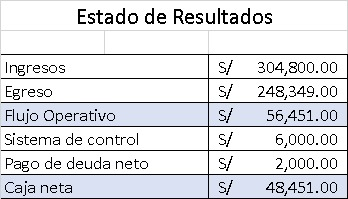
\includegraphics[width=0.8\textwidth]{anexos/er.jpeg}
	% \caption{Flujo de Efectivo}
	% 	\label{fig:flujo-efectivo}
	% \end{figure}

	% \begin{figure}[H]
	% 	\centering
	% 	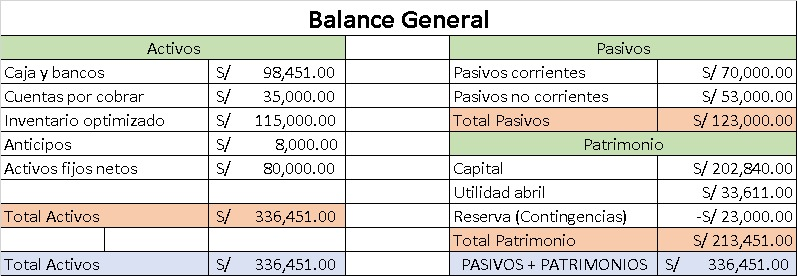
\includegraphics[width=0.8\textwidth]{anexos/bg.jpeg}
	% 	\caption{Balance General}
	% 	\label{fig:balance-general}
	% \end{figure}

	% \begin{figure}[H]
	% 	\centering
	% 	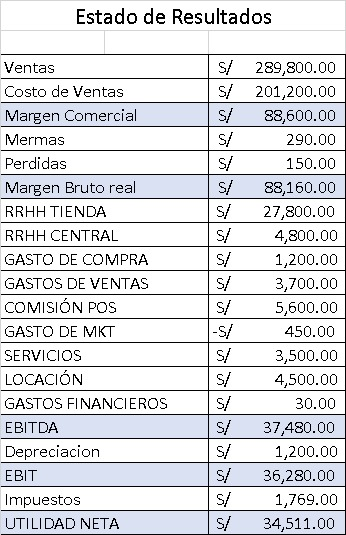
\includegraphics[width=0.8\textwidth]{anexos/fe.jpeg}
		
	% 		\caption{Estados de Resultados}
	% 	\label{fig:estados-Resultados}
	% \end{figure}

%\chapter{Anexo II: Resumen de Papers investigados}
%%\section{Conclusiones}
%
%\begin{table}[h]
%	\newcommand{\multirot}[1]{\multirow{2}{*}[-8ex]{\rotcell{\rlap{#1}}}}
%	%\scriptsize
%	\footnotesize
%	\centering
%	\begin{tabular}{|m{0.5cm}|m{0.3cm}|m{4cm}|m{2cm}|m{0.6cm}|m{1.7cm}|m{3cm}|} 
%		\hline
%		\rowcolor[rgb]{0,0.251,0.502} \multicolumn{1}{|c|}{\textcolor{white}{Tipo}} & \multicolumn{1}{c|}{\textcolor{white}{N°}} & \multicolumn{1}{c|}{\textcolor{white}{Título}}                                                                             & \multicolumn{1}{c|}{\textcolor{white}{Autor}}        & \multicolumn{1}{c|}{\textcolor{white}{Año}} & \multicolumn{1}{c|}{\textcolor{white}{País}} & \multicolumn{1}{c|}{\textcolor{white}{Fuente}}                                                        \\ 
%		\hline
%		\multirot{Problema}                                        & 1                                             & Copper price estimation using bat algorithm~                                                                               & Dehghani  Bogdanovic                                 & 2018                                        & United Kingdom                               & Resources Policy                                                                                      \\ 
%		\cline{2-7}
%		& 2                                             & Alternative techniques for forecasting mineral commodity prices                                                            & Cortez, Saydam, Coulton,  Sammut                     & 2018                                        & Netherlands                                  & International Journal of Mining Science and Technology                                                \\ 
%		\hline
%		\multirow{3}{*}[-14ex]{\rotcell{\rlap{Propuesta}}}
%		& 3                                             & Prediction of the crude oil price thanks to natural language
%		processing applied to newspapers~                           & Trastour, Genin,  Morlot                             & 2016                                        & USA                                          & Standfort University ML repository                                                                    \\ 
%		\cline{2-7}
%		& 4                                             & Stock Price Prediction Using Deep Learning~                                                                                & Tipirisetty                                          & 2018                                        & USA                                          & Master's Theses San Jose State University                                                             \\ 
%		\cline{2-7}
%		& 5                                             & Deep Learning for Stock Prediction Using Numerical and Textual
%		Information                                               & Akita, R., Yoshihara, A., Matsubara, T.,  Uehara, K. & 2016                                        & USA                                          & 2016 IEEE/ACIS 15th International Conference on Computer and
%		Information Science (ICIS)             \\ 
%		\hline
%		\multirow{4}{*}[-28ex]{\rotcell{\rlap{Técnica}}}                                          & 6                                             & Stock Prices Prediction using the Title of Newspaper Articles
%		with Korean Natural Language Processing~                   & Yun, Sim,  Seok                                      & 2019                                        & Japan                                        & 2019 International Conference on Artificial Intelligence in
%		Information and Communication (ICAIIC)  \\ 
%		\cline{2-7}
%		& 7                                             & A Method of Optimizing LDA Result Purity Based on Semantic
%		Similarity                                                    & Jingrui, Z., Qinglin, W., Yu, L.,  Yuan, L.          & 2017                                        & China                                        & 2017 32nd Youth Academic Annual Conference of Chinese
%		Association of Automation (YAC)~              \\ 
%		\cline{2-7}
%		& 8                                             & Qualitative Stock Market Predicting with Common Knowledge Based
%		Nature Language Processing: A Unified View and Procedure & Rao, D., Deng, F., Jiang, Z.,  Zhao, G.~             & 2015                                        & USA                                          & 2015 7th International Conference on Intelligent Human-Machine
%		Systems and Cybernetics              \\ 
%		\cline{2-7}
%		& 9                                             & Fuzzy Bag-of-Words Model for Document Representation                                                                       & Zhao, R.,  Mao, K.                                   & 2018                                        & USA                                          & IEEE Transactions on Fuzzy Systems (~Volume:
%		26~,~Issue: 2~, April 2018~)                           \\
%		\hline
%	\end{tabular}
%	\caption{Cuadro Resumen de Papers investigados. Fuente: Elaboración propia}
%\label{A:table}
%\end{table}





	% \clearpage
	%%%Bibliografia
	%\bibliographystyle{apalike} % Title is link if provided
	%\renewcommand{\bibname}{BIBLIOGRAFÍA} % changes the header; default: Bibliography
	

	\printbibliography[heading=bibintoc,title={BIBLIOGRAFÍA}]
	%\bibliography{tesisblx.bib} % adjust this to fit your BibTex file
	
\end{document}
